% !TEX encoding = UTF-8 Unicode
\chapter{Simulation results}  \label{chap-simulation}
%
This chapter describes numerical simulations carried out to demonstrate and evaluate the disturbance models and observer designs described in Chapter \ref{chap-methods}. Section \ref{sec:sim-RODDs} presents a few simulated examples of different \gls{RODD}s. Section \ref{sec:sim-obs-lin} describes experiments to evaluate the multiple-model observers in estimating the states of two simulated systems, a single-input single-output (SISO) linear system with one \gls{RODD} step disturbance, and a 2-input, 2-output linear system with two \gls{RODD} step disturbances. Section \ref{sec:sim-ore-SISO} describes an experiment to evaluate the observer performance on the simulated grinding circuit model with one output variable and a step disturbance in the ore feed mix. %\textcolor{red}{Section \ref{sec:sim-ore-mimo-ctrl} describes an experiment to evaluate the observers in a multi-variable feedback control scenario with the simulated grinding circuit model.}


\section{Generating RODD disturbances} \label{sec:sim-RODDs}

\gls{RODD}s are easy to generate by numerical simulation.  Plot (a) in Figure \ref{fig:rodd-sim-plots} shows a random shock sequence (\ref{eq:wpk1}) of length 1000 samples generated using a pseudo-random number generator. Plots (b), (c), and (d) show step, ramp and exponential change disturbances generated with this random shock sequence using the \gls{RODD} models in (\ref{eq:RODD-step}), (\ref{eq:RODD-ramp}), and (\ref{eq:RODD-exp}). Figure \ref{fig:rodd-sim-plot2} shows a combined RODD with abruptly changing ramps and steps (\ref{eq:RODD-step-ramp}).
\begin{figure}[htp]
	\centering
	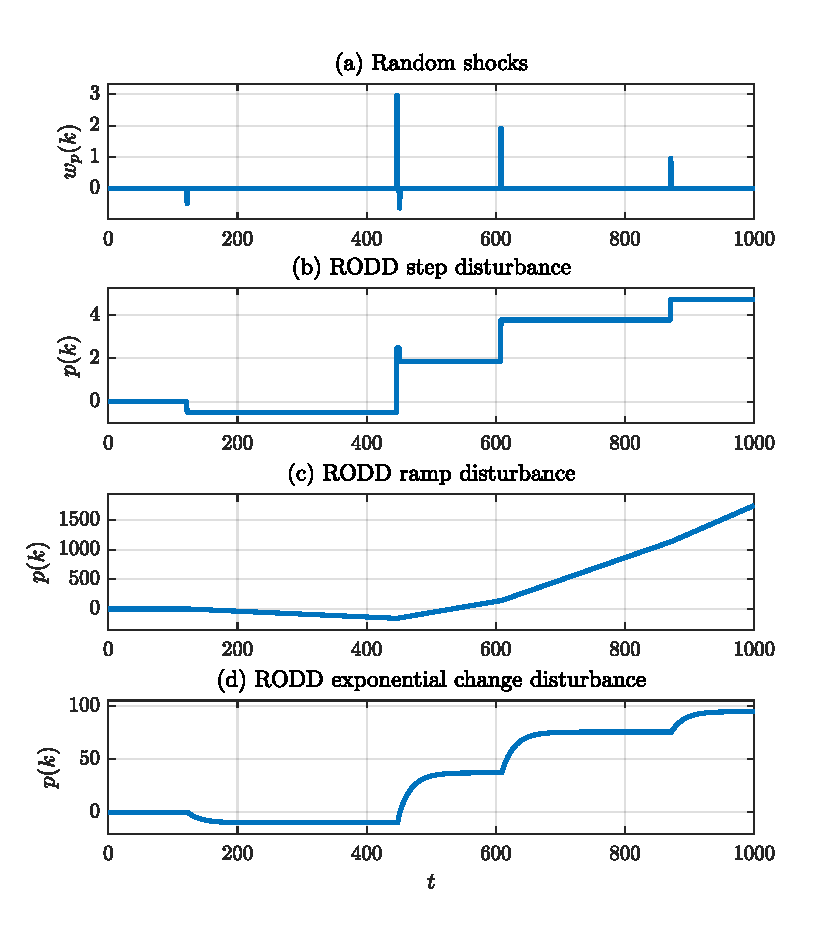
\includegraphics[width=13cm]{images/rodd_sim_plots.pdf}
	\caption{Examples of \gls{RODD}s}
	\label{fig:rodd-sim-plots}
\end{figure}
\begin{figure}[htp]
	\centering
	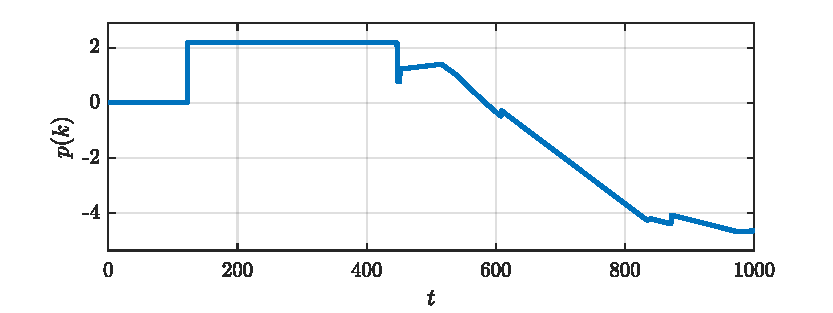
\includegraphics[width=13cm]{images/rodd_sim_plot2.pdf}
	\caption{A \gls{RODD} with steps and ramps}
	\label{fig:rodd-sim-plot2}
\end{figure}


\section{Observer evaluation with linear systems} \label{sec:sim-obs-lin}

\subsection{SISO linear system} \label{sim-obs-lin-1}

To demonstrate state estimation in the presence of \gls{RODD}s, a single \gls{RODD} was simulated at the input to a SISO process represented by a discrete-time linear model, as shown in the functional diagram in Figure \ref{fig:sim-sys-diag-siso}. In addition to the unmeasured \gls{RODD}, $p(k)$, the process has a known input, $u(k)$, and a measured output, $y_M(k)$. The measurements are simulated by adding a random noise, $v(k)$, with zero mean and standard deviation, \gls{sigmaM}, to the output of the process. At each sample time, the input and measured output are passed to an observer, which calculates estimates of the process states, $\hat{\mathbf{x}}(k|k)$, and an estimate of the process output, $\hat{y}(k|k)$. % TODO: add glossary items for SISO variables.
\begin{figure}[htp]
	\centering
	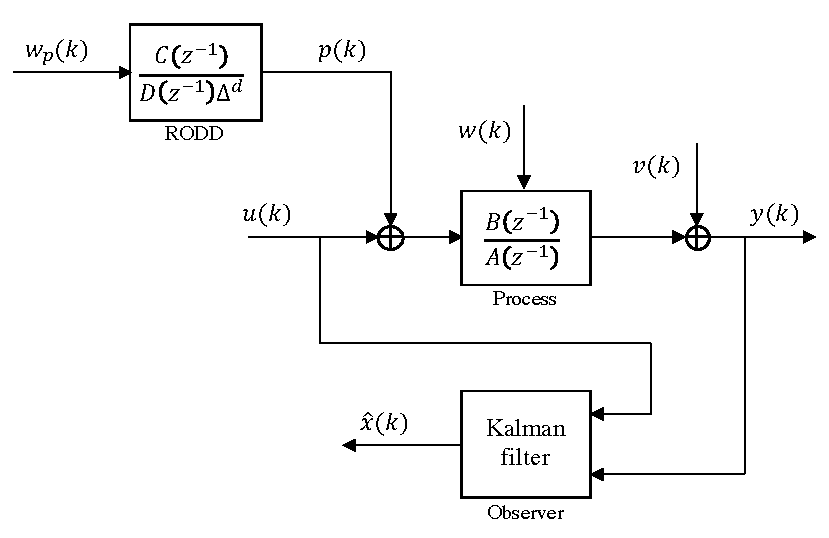
\includegraphics[width=11.5cm]{images/sim-sys-diag-siso.pdf}
	\caption{Functional diagram of the simulated \gls{SISO} system with observer}
	\label{fig:sim-sys-diag-siso}
\end{figure}

For the purposes of this experiment, the linear model used to represent the process was the stable first order system,
\begin{equation}
	\frac{B(q^{-1})}{A(q^{-1})} = \frac{0.3q^{-1}}{1-0.7q^{-1}}
\end{equation}
with a sampling period, \gls{Ts}, of 0.5.

The \gls{RODD} was a step disturbance created by setting
\begin{equation}
	\frac{C(q^{-1})}{D(q^{-1})} = \frac{1}{1-q^{-1}}.
\end{equation}
The random shock, \gls{wpk}, was defined by (\ref{eq:wpik2}) with $\gls{epsilon}=0.01$, $\gls{sigmawp}=0.01$, and $\gls{b}=100$.

The state-space model used to simulate the augmented system was
\begin{equation} \label{eq:sim-sys-siso-ss-aug}
	\begin{split}
	\mathbf{x}_{a}(k+1) & =\left[\begin{array}{cc}
		0.7 & 1 \\
		0 & 1
	\end{array}\right] \mathbf{x}_{a}(k)+\left[\begin{array}{l}
		1 \\
		0
	\end{array}\right] u(k) + \mathbf{w}_{a}(k) \\
	y(k) & =\left[\begin{array}{cc}
	0.3 & 0
\end{array}\right] \mathbf{x}_{a}(k) + v(k)
\end{split}
\end{equation}
where
\begin{equation} \label{eq:sim-sys-siso-ss-aug2}
		\mathbf{x}_{a}(k) = \left[\begin{array}{l}
			x_{a,1}(k) \\
			x_{a,2}(k)
		\end{array}\right] = \left[\begin{array}{l}
		x_{1}(k) \\
		p(k)
	\end{array}\right], \mathbf{w}_{a}(k) = \left[\begin{array}{l}
	w(k) \\
	w_{p}(k)
\end{array}\right] .
\end{equation}

Note that with this representation, the second model state $x_{a,2}(k)$ corresponds exactly to the input disturbance $p(k)$.

\subsection{Analysis of sub-optimal estimators} \label{sim-obs-lin-1-SKF-analysis}

To understand and investigate the behaviour of the observers, the system (\ref{eq:sim-sys-siso-ss-aug}) was first simulated for 100 sample periods with two pre-determined shocks, no persistent disturbance ($\sigma_{w_p}=0$), and no measurement noise ($\sigma_M=0$). Figure \ref{fig:rod-obs-sim-test-ioplot-SF95} shows the simulation data. The two lower plots show the system inputs, including the random shock signal. The upper two plots show the system states and outputs as well as the estimates of a sub-optimal multiple-model observer using the sequence fusion algorithm described by \cite{robertson_detection_1995} with parameters $\gls{nf}=15$, $\gls{m}=1$, and $\gls{d}=5$.
\begin{figure}[htp]
	\centering
	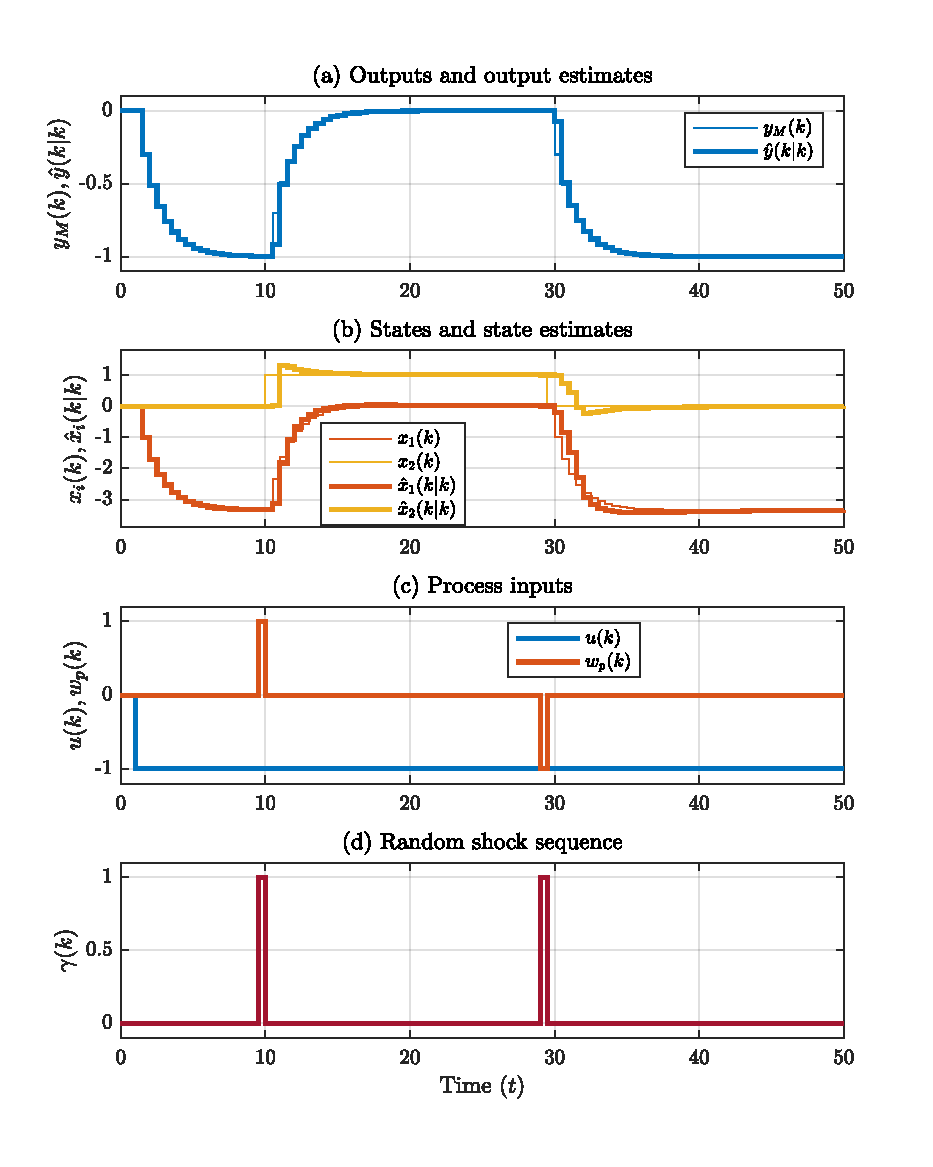
\includegraphics[width=13cm]{images/rod_MKF_SF_test_sim_MKF_SF95_ioplot.pdf}
	\caption{Simulation of a SISO linear system with a \gls{RODD} input disturbance}
	\label{fig:rod-obs-sim-test-ioplot-SF95}
\end{figure}

\begin{figure}[htp]
	\centering
	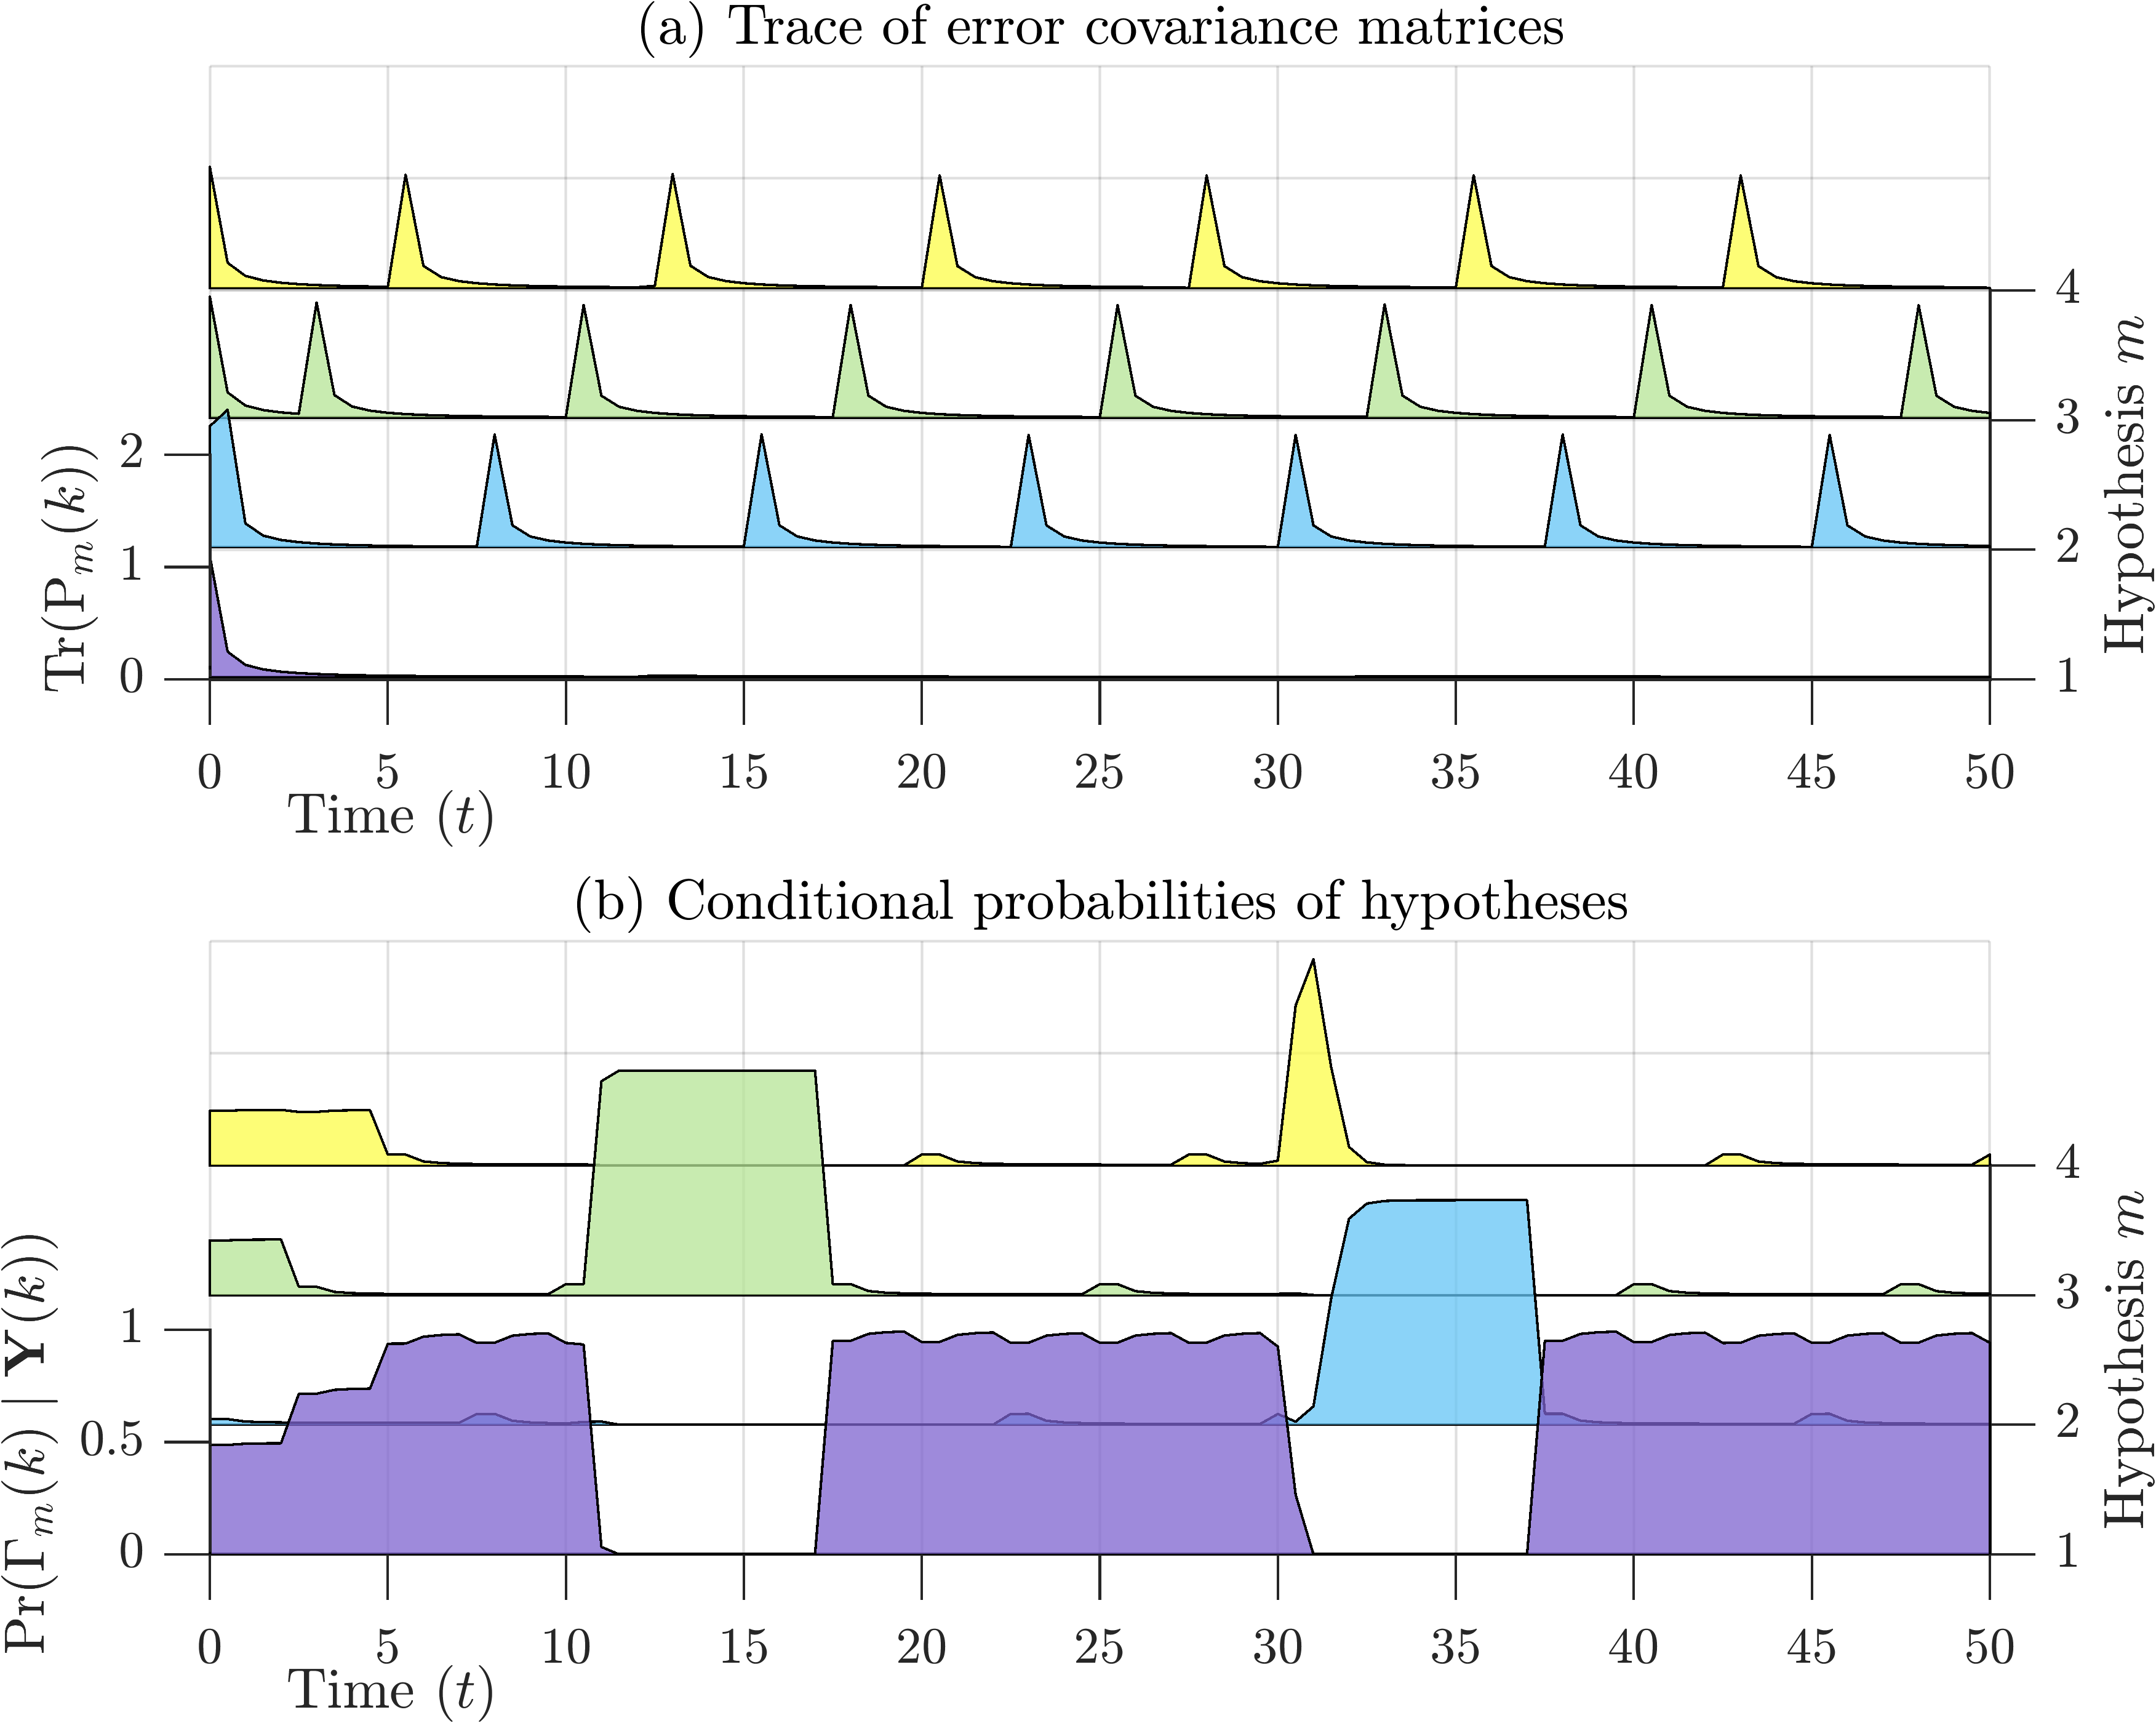
\includegraphics[width=12cm]{images/rod_MKF_test_sim_MKF_SF95_prob.png}
	\caption{Multi-model observer probability estimates – MKF--SF95}
	\label{fig:rod-obs-sim-test-probs-SF95}
\end{figure}
The two plots in Figure \ref{fig:rod-obs-sim-test-probs-SF95} provide insight into the computations of the observer, which is labelled `MKF--SF95'. The upper plot shows four time series of the trace (i.e. the sum of the elements on the main diagonal) of the merged error covariance matrices, $\mathbf{P}_m(k)$ for $m=1,2,...,n_m$. The diagonal values of $\mathbf{P}_m(k)$ may be interpreted as indicators of the magnitude of the errors of the state estimates. Recall that $\mathbf{P}_m(k)$ is time-varying and influenced by the process noise covariance, $\mathcal{Q}(\gamma_f(k))$, which switches according to the hypothesis sequences (\ref{eq:Pfkp1}). In this simulation, the covariances at time $t=0$ were initialized to the identity matrix ($\mathbf{P}_m(0)=\mathbf{I}_2$). It can be seen that the trace values initially drop rapidly and tend towards zero, however, at certain times, they increase sharply to a peak before dropping again. The sharp peaks are caused by the shock hypotheses ($\gamma_m(k)=1$) of the sequences.

The lower plot shows the conditional likelihood estimates of the four hypotheses given the data up to time $k$ after the merging step (\ref{eq:xmkymk_hat_MKF}). The conditional likelihoods were initialized with equal values ($\operatorname{Pr}\left(\Gamma_m(0) \mid \mathbf{Y}_M(0)\right)=1/n_m$). It can be seen that the likelihoods of each hypothesis settle on a steady-state by $t=5$ and hypothesis 1 dominates the probability distribution until $t=10$. This means that the merged estimates of the observer are determined almost completely by hypothesis 1 during this period. This makes sense since hypothesis 1 represents a sequence containing no shocks and the first shock does not occur until $t=9.5$. A short time after the first shock, the probability density shifts to hypothesis sequence 3 which happens to assume a shock at $t=10$. This is evident in the upper plot where it can be seen that the error covariance of hypothesis 3 increases and peaks at $t=10.5$. The probability switches from hypothesis 1 to 3 by $t=11.5$ and remains there until $t=17$ when it shifts back to hypothesis 1. This final shift can be explained by the fusion horizon, \gls{nf}, which in this case is 15 sample periods or 7.5 time units. Hypothesis 3 assumes another shock occurs at this time, which is not the case. Therefore, hypothesis 1 becomes the most likely hypothesis after that. The second shock occurs at $t=29$, which is not as favourable since it does not align well with the shocks in any of the hypothesis sequences. Initially, the likelihood switches to hypotheses 4, which assumes a shock at $t=27.5$ but then it switches to hypothesis 2, which assumes a shock at $t=30$. Again, the probability remains high until the next shock is scheduled, at which point hypothesis 1 becomes the most likely again.

\begin{figure}[htp]
	\centering
	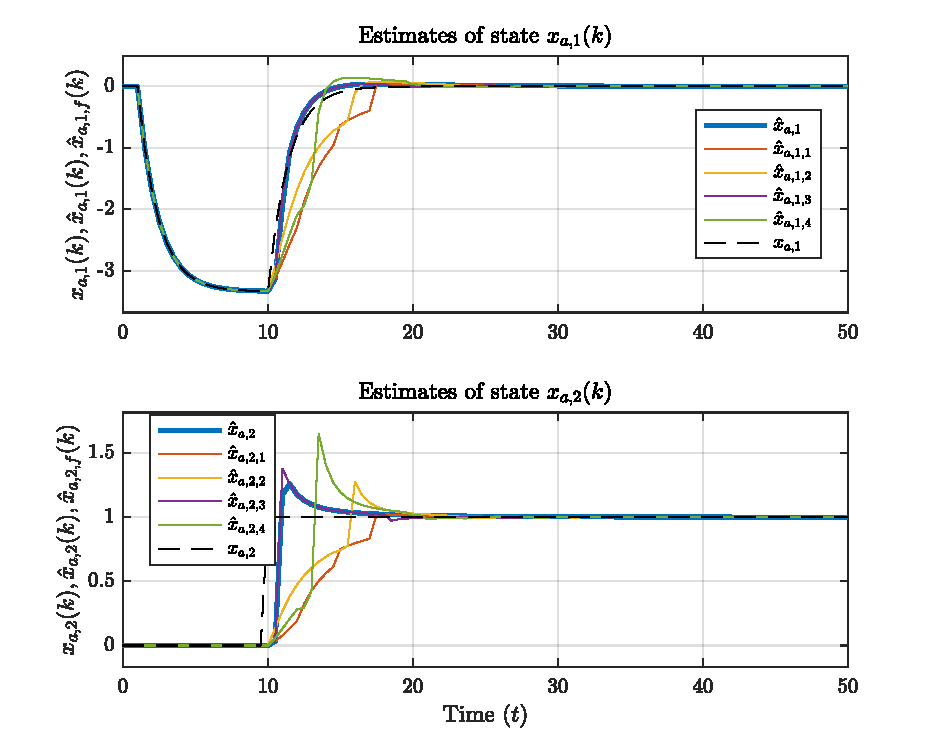
\includegraphics[width=13cm]{images/rod_MKF_test_sim_MKF_SF95_x_est.pdf}
	\caption{Multi-model observer state estimates – MKF--SF95}
	\label{fig:rod-obs-sim-test-x_est-SF95}
\end{figure}
Figure \ref{fig:rod-obs-sim-test-x_est-SF95} shows the merged state estimates associated with each hypothesis (thin coloured lines), as well as the overall state estimate (thick blue lines) and the true states of the system (dashed lines). These plots reveal the role that each hypothesis plays in the overall estimates. The estimates of hypothesis 3 (purple lines) are the first to respond to the first shock at time $t=9.5$ and the overall estimate closely follows this hypothesis. The other estimates (green, yellow and orange lines) respond at later intervals and do not play a role in the overall estimate. After the second shock occurs, the overall estimate follows that of hypothesis 4 at first, then it switches to 2, however, it lags the true system state and the response of the output estimate is slower and overshoots the true system output for a few time steps. These simulation results demonstrate that the performance of the sequence fusion algorithm is somewhat sensitive to the timing of the true shocks.

As described in Section \ref{sec:fusion}, Robertson and coworkers proposed an alternative implementation of the sequence fusion algorithm \citep{robertson_method_1998}. There are two differences between this and the previous algorithm. Firstly, shocks are assumed to act over the duration of the detection interval rather than at one sample time within it. Secondly, the variance of the shocks, $\gls{b}^2\gls{sigmawp}^2$, is reduced according to the interval length, (\ref{eq:wpdk}).
%% TODO: add parameters to above? with $f=15$ $m=1$ and $d=5$.

\begin{figure}[htp]
	\centering
	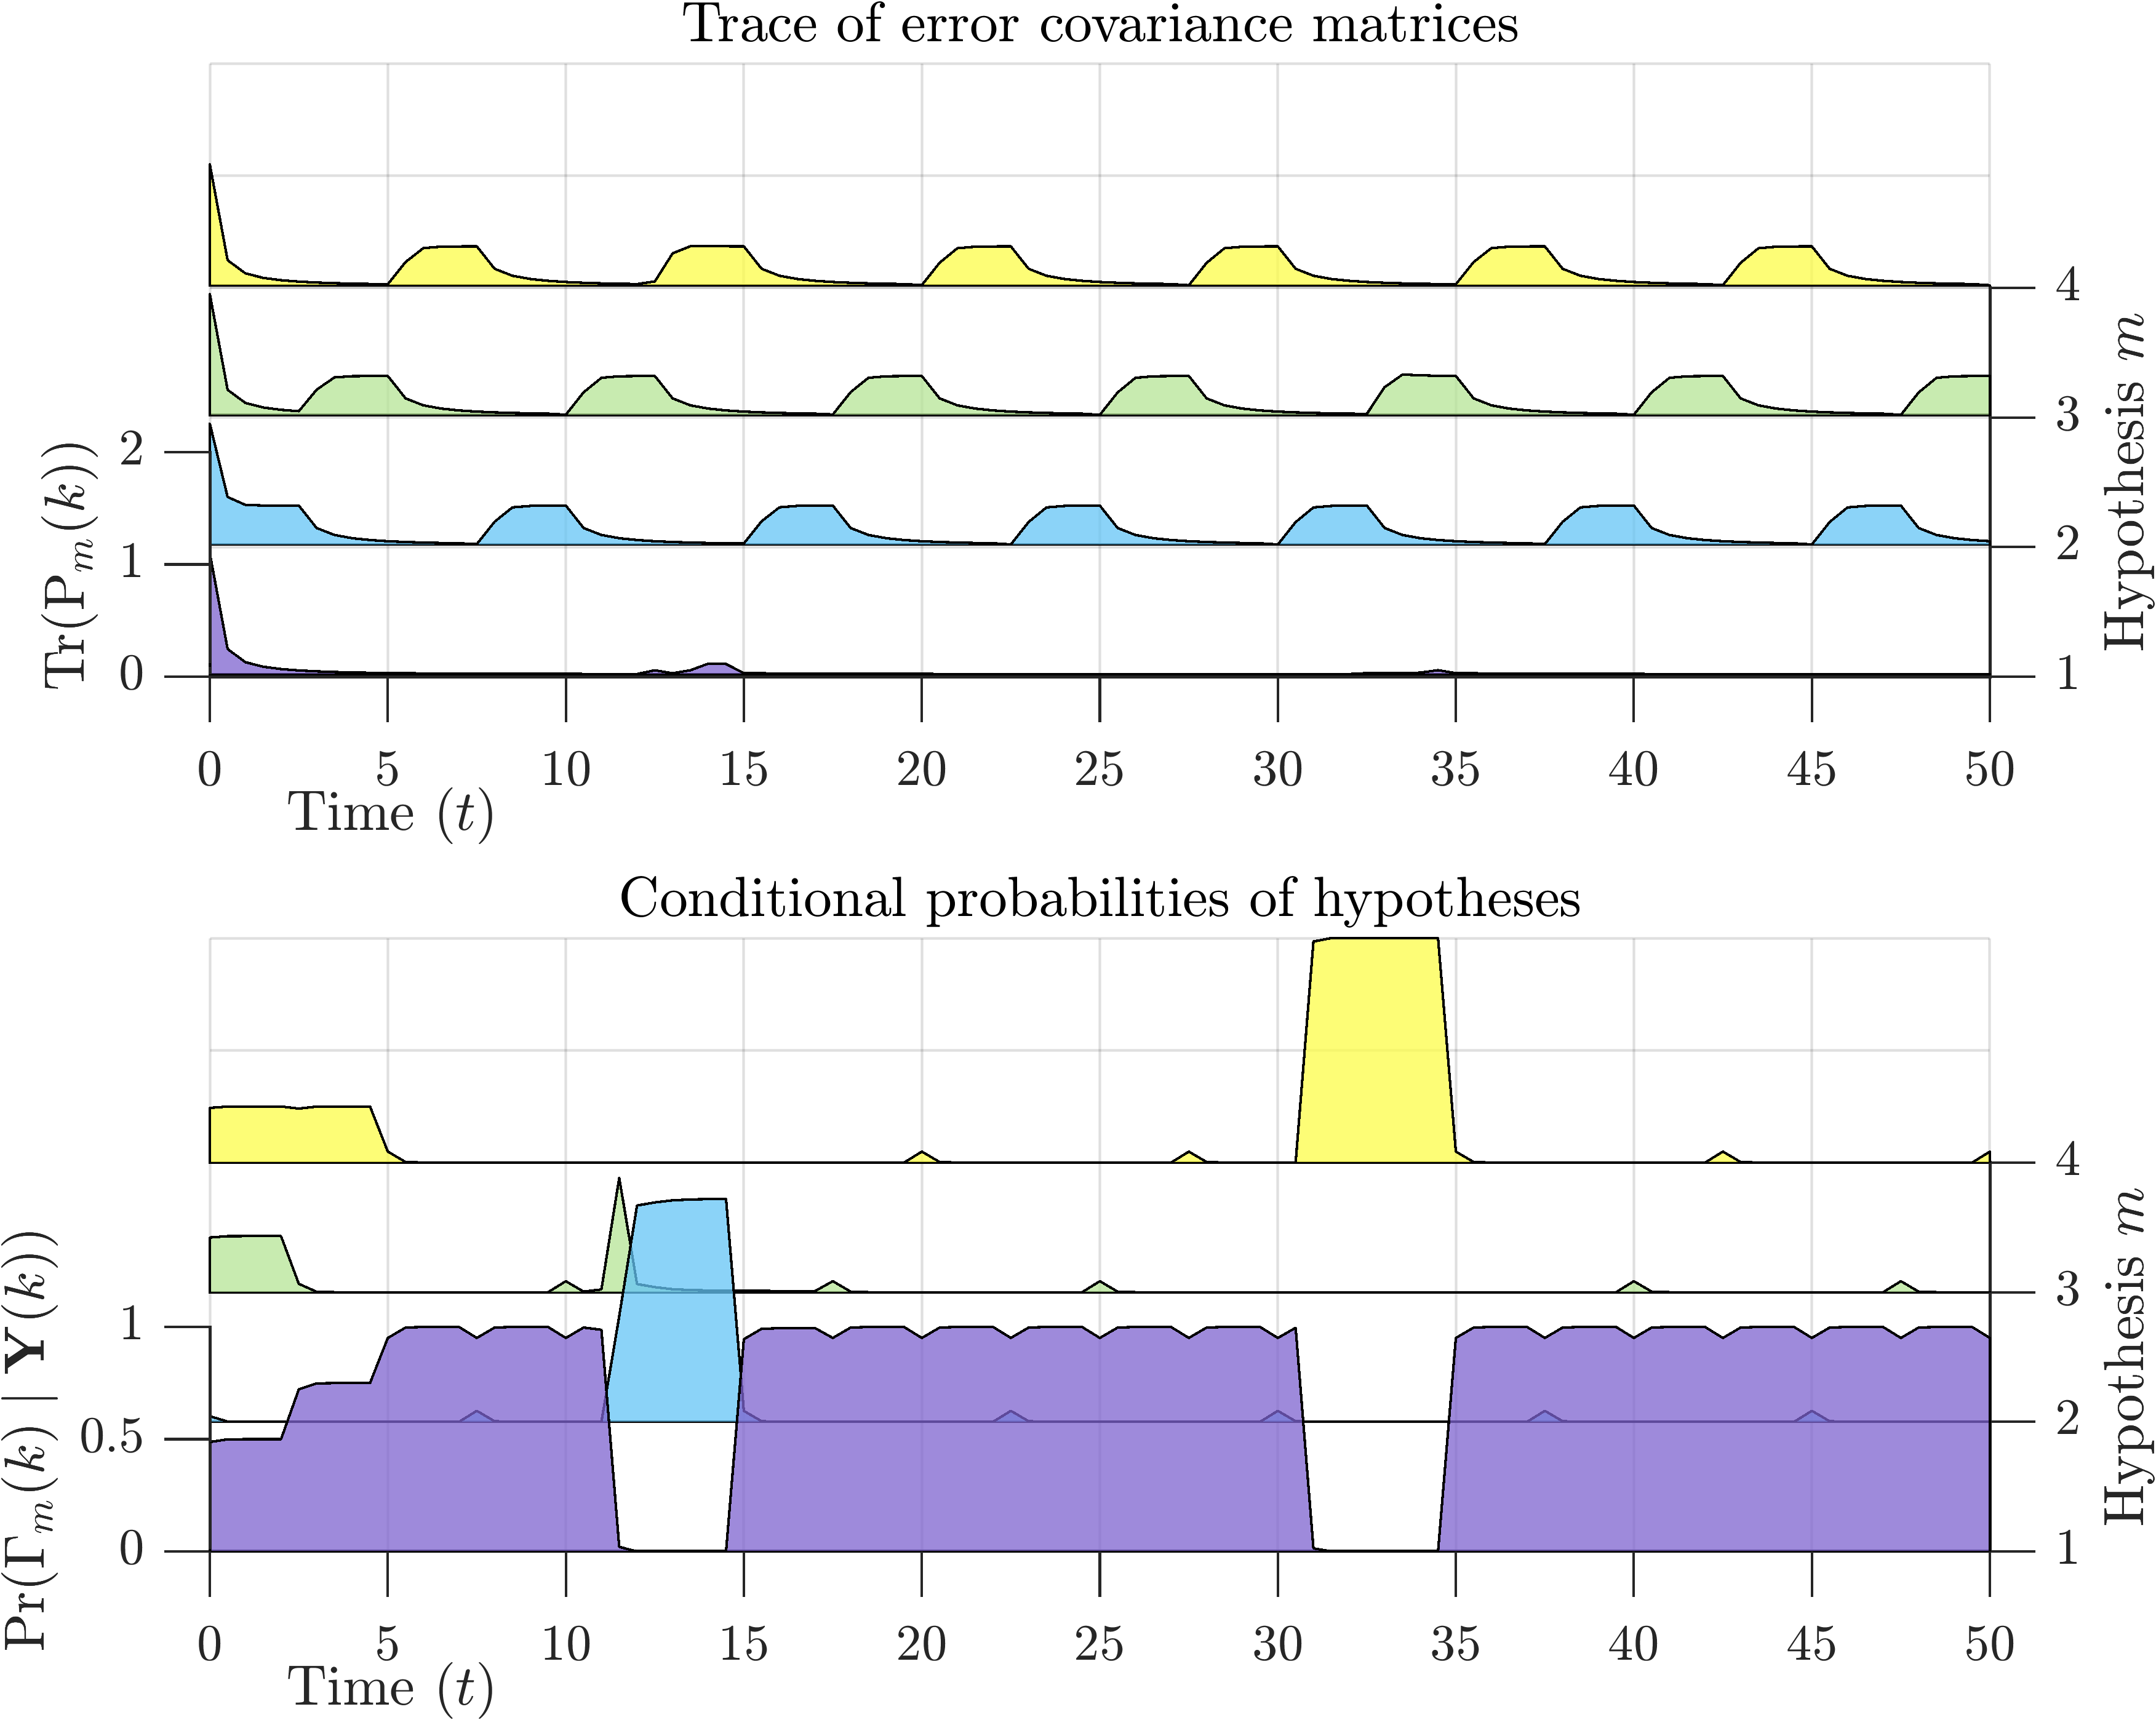
\includegraphics[width=12cm]{images/rod_MKF_test_sim_MKF_SF98_prob.png}
	\caption{Multi-model observer probability estimates – MKF--SF98}
	\label{fig:rod-obs-sim-test-probs-SF98}
\end{figure}
Figures \ref{fig:rod-obs-sim-test-probs-SF98} and \ref{fig:rod-obs-sim-test-x_est-SF98} show the results of simulating the 1998 version of the observer, labelled `MKF--SF98', with the same simulation data. The effect of the modifications on the error covariance is clear. The traces of the error covariance peak at a lower value and the peaks are sustained for the duration of the detection intervals, unlike in the 1995 version. The switching of the hypothesis probabilities is also different. After the first shock at $t=9.5$ the probability shifts to hypothesis 2 rather than 3. This may be due to the fact that the shock occurred in the middle of the detection interval of hypothesis 2. After the second shock at $t=29$ the hypothesis 4 becomes the most probable.

Figure \ref{fig:rod-obs-sim-test-x_est-SF98} shows the merged state estimates of each hypothesis, the overall estimates, and the true system states for the 1998 version of the algorithm. The estimates responding quickly to the shocks and there is noticeably less overshoot of the estimates in this simulation compared to the 1995 version.   
\begin{figure}[htp]
	\centering
	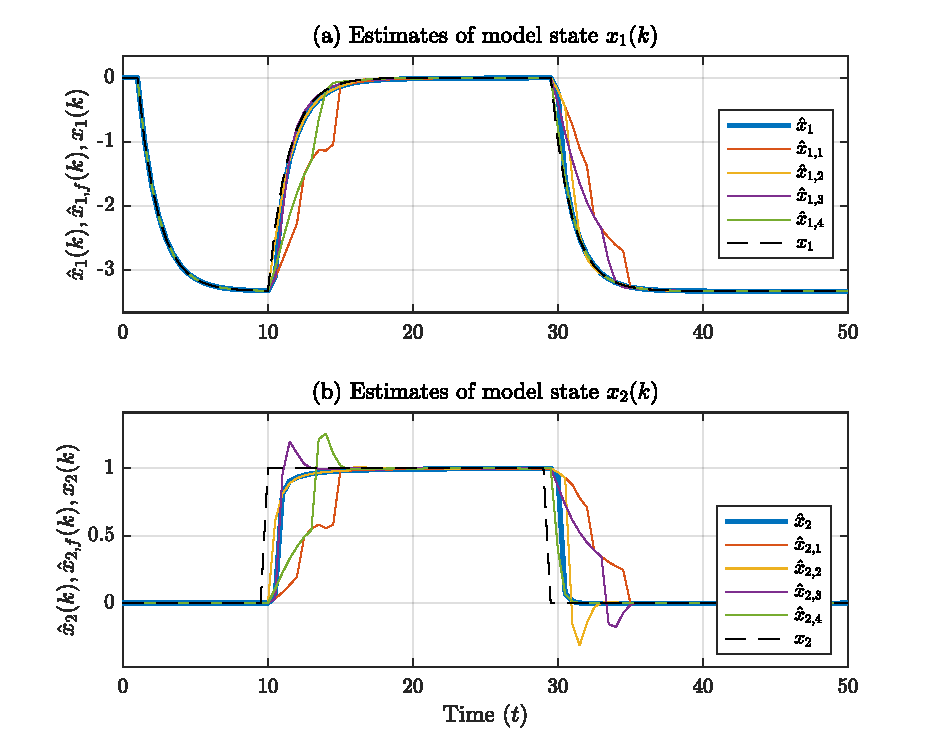
\includegraphics[width=13cm]{images/rod_MKF_test_sim_MKF_SF98_x_est.pdf}
	\caption{Multi-model observer state estimates – MKF--SF98}
	\label{fig:rod-obs-sim-test-x_est-SF98}
\end{figure}

\begin{figure}[htp]
	\centering
	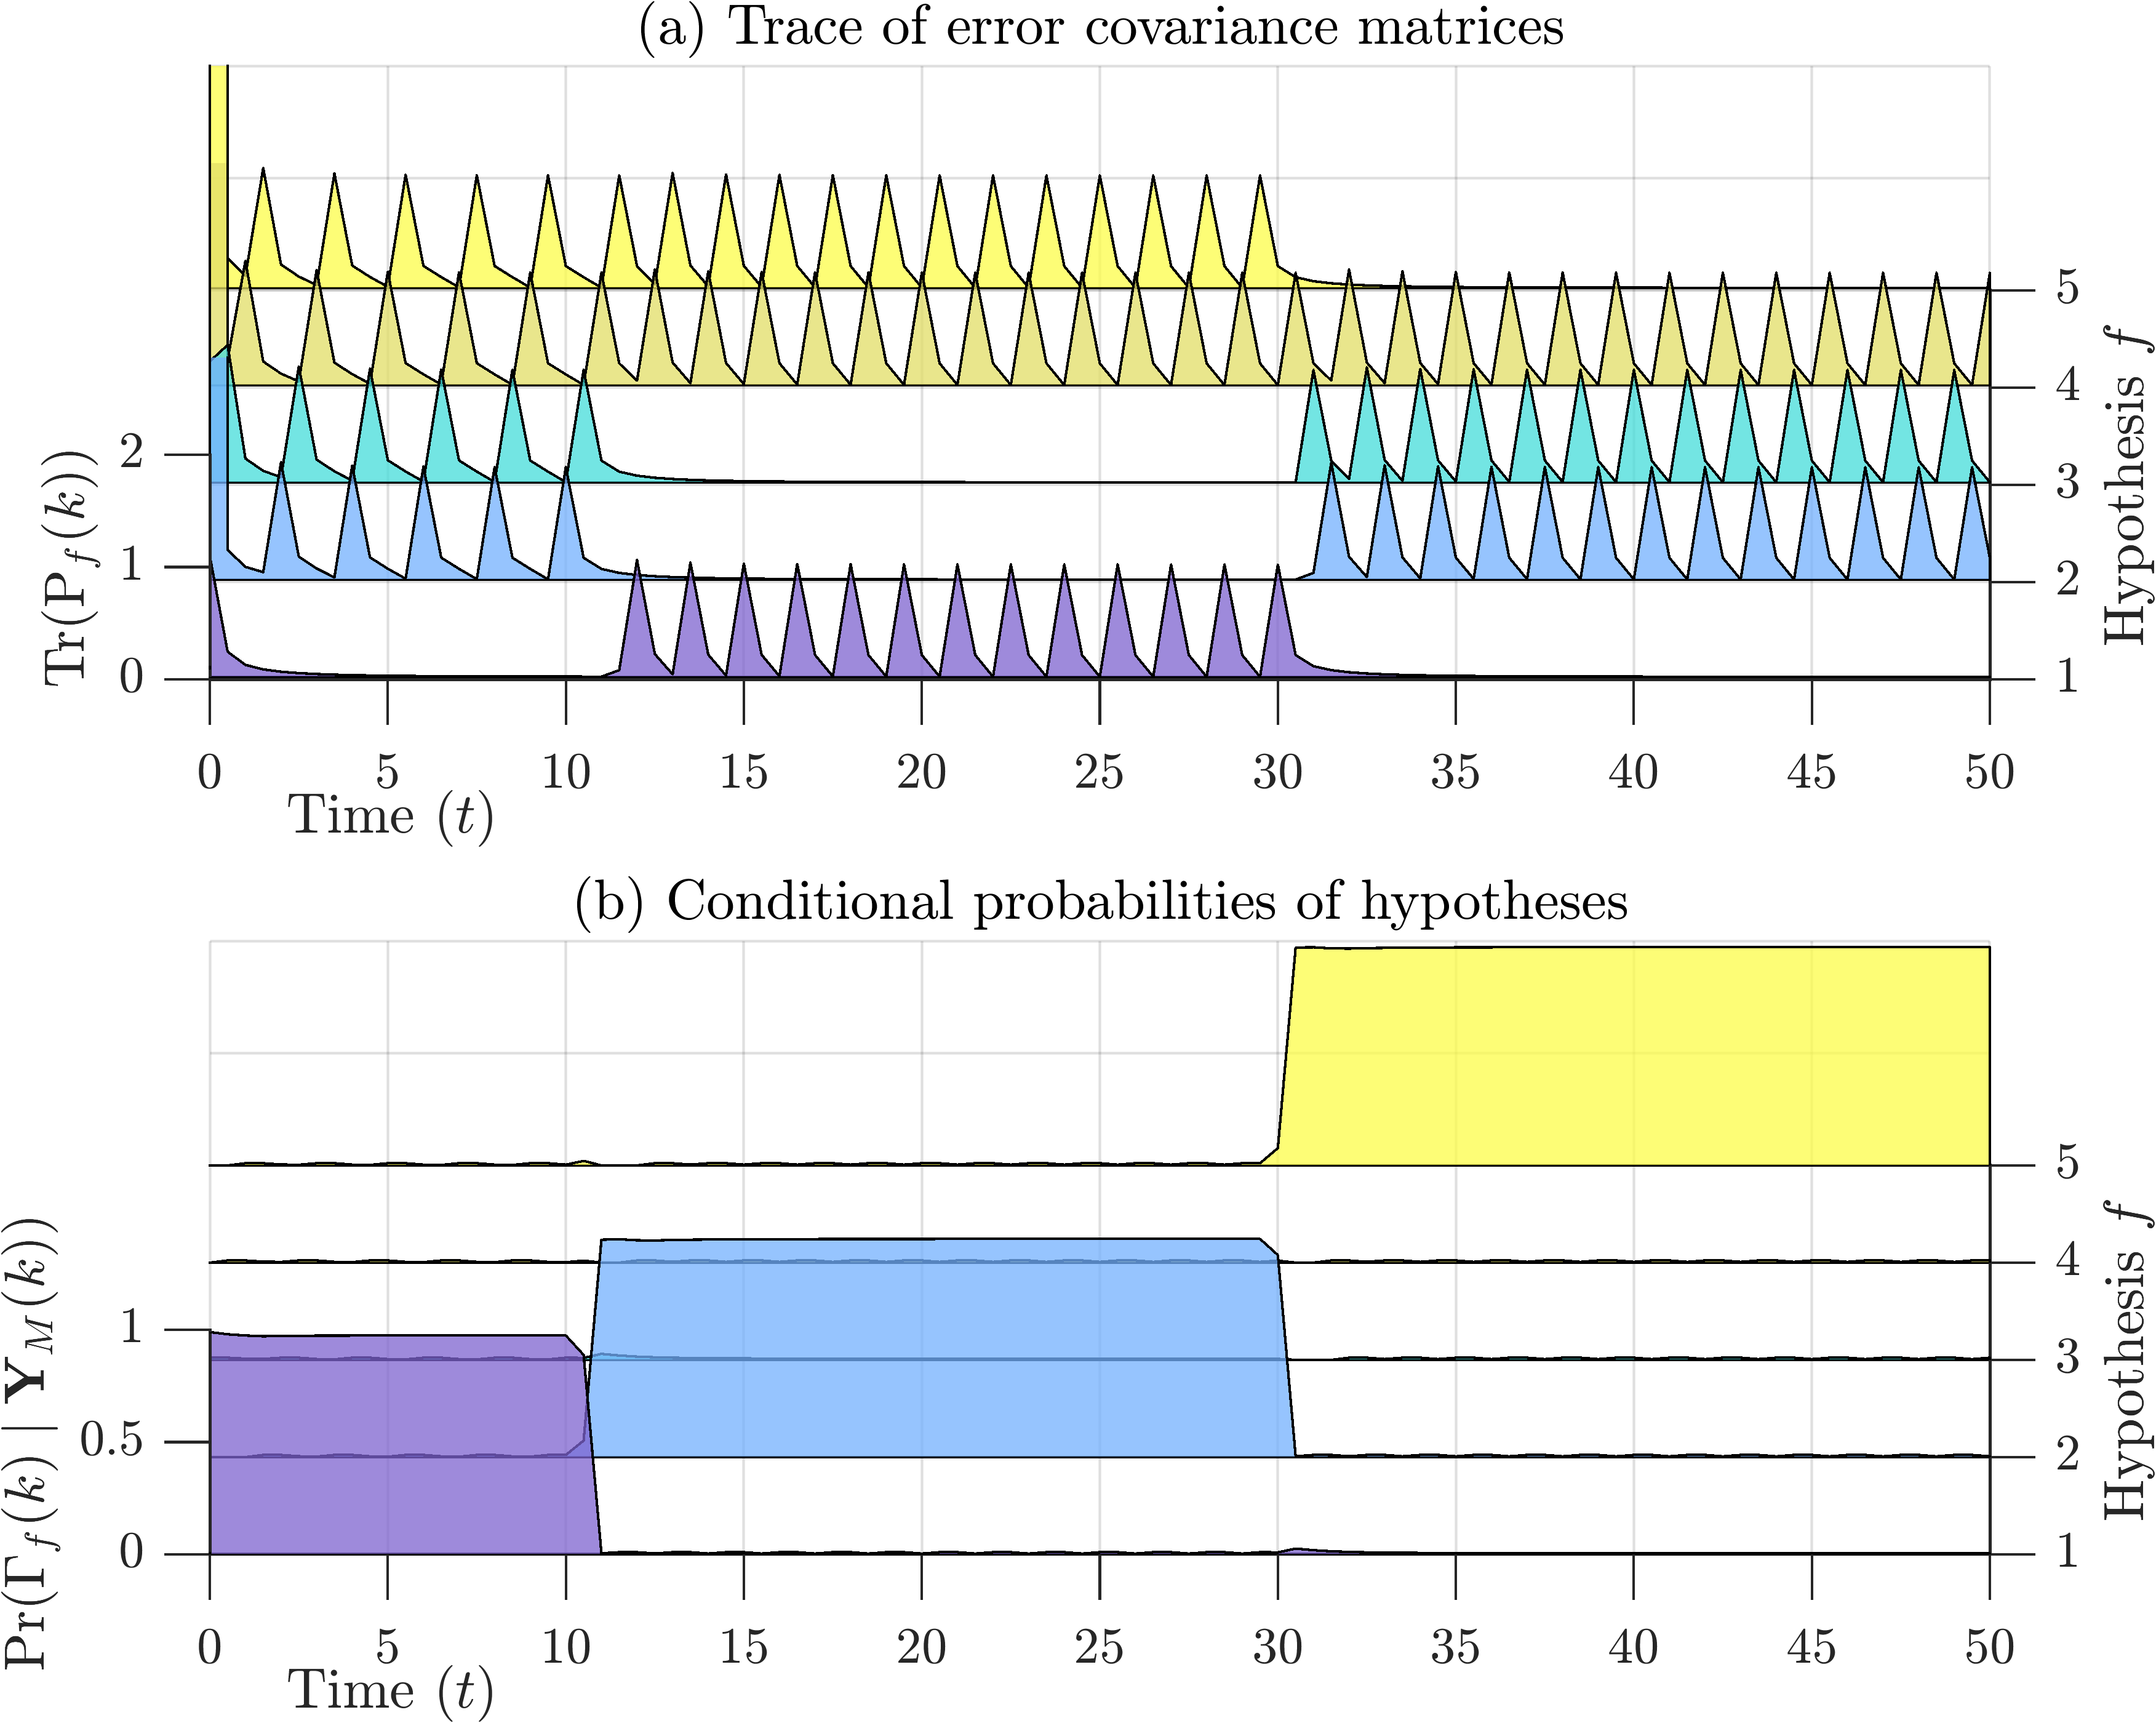
\includegraphics[width=12cm]{images/rod_MKF_test_sim_MKF_SP_prob.png}
	\caption{Multi-model observer probability estimates – MKF--SP}
	\label{fig:rod-obs-sim-test-probs-SP}
\end{figure}
\begin{figure}[htp]
	\centering
	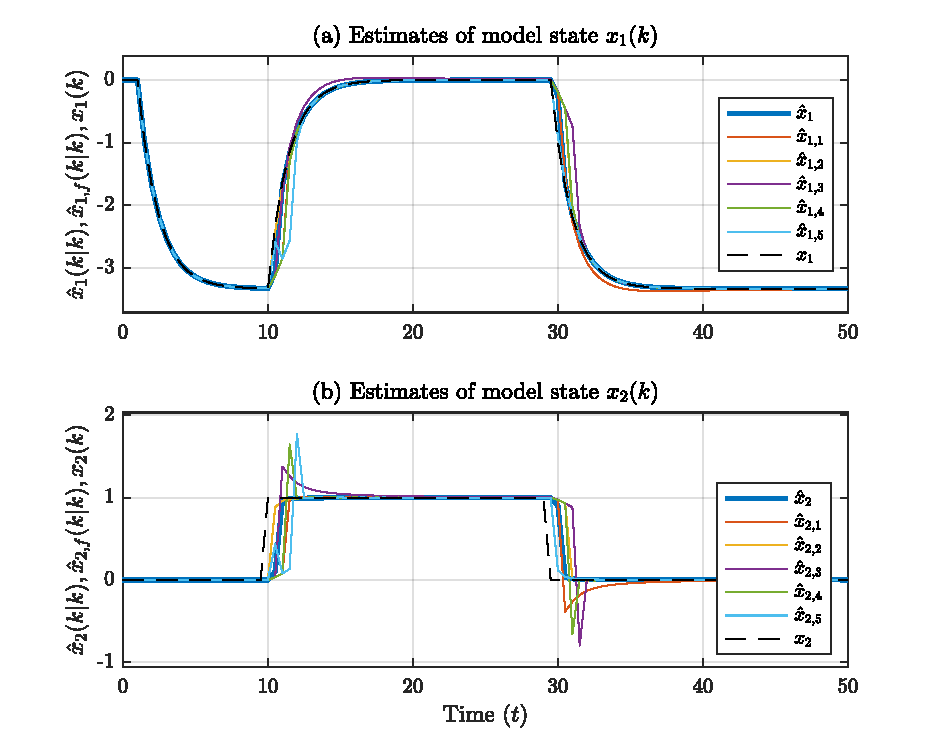
\includegraphics[width=13cm]{images/rod_MKF_test_sim_MKF_SP_x_est.pdf}
	\caption{Multi-model observer state estimates – MKF--SP}
	\label{fig:rod-obs-sim-test-x_est-SP}
\end{figure}
Figures \ref{fig:rod-obs-sim-test-probs-SP} and \ref{fig:rod-obs-sim-test-x_est-SP} show the corresponding results of simulating the sequence pruning multiple-model observer, labelled `MKF--SP', with $\gls{nh}=5$ and $\gls{nmin}=2$, as described by \cite{eriksson_classification_1996}. Recall that in this algorithm, hypotheses are adaptively pruned and replaced at every sample time. From these plots it can be seen that the hypotheses include more possible shocks than those modelled by the sequence fusion observers with detection intervals. Also, the switching of hypothesis probabilities is swifter and distinct, and the estimation errors are visibly lower than those of both versions of the sequence fusion observer in these simulations.

To effectively evaluate and compare the performance of these observers, longer simulations with pseudo-random shocks and measurement noise are needed. Figure \ref{fig:rod-obs-sim1-ioplot} shows the first 600 input-output samples from a simulation of the system with a total duration of 2500 (5000 samples). The lower plot shows the input signals, $u(k)$ and $p(k)$, from which it can be seen that two significant random shocks occurred during this period (at $t=98$ and $220.5$). At other times, the value of $p(k)$ is a random walk due to the persistent component of the \gls{RODD} disturbance (\ref{eq:wpk2}). In addition, a step change in $u(k)$ of magnitude 1 occurred at time $t=5$. The upper plot shows the simulated output measurements. The standard deviation of the measurement noise, \gls{sigmaM}, was $0.1$. No disturbances other than $w_p(k)$ were simulated (i.e. $w_1(k)=0$).
\begin{figure}[htp]
	\centering
	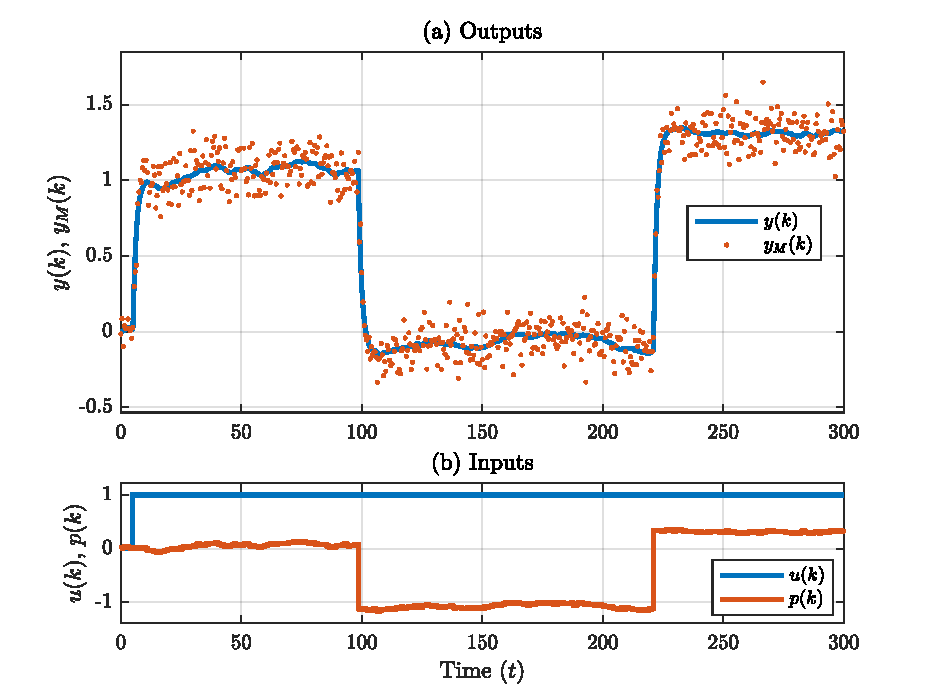
\includegraphics[width=13cm]{images/rod_obs_sim1_all_seed_ioplot.pdf}
	\caption{Simulation of linear system with a \gls{RODD} input disturbance}
	\label{fig:rod-obs-sim1-ioplot}
\end{figure}

\subsubsection{Tuning of Kalman filters} \label{sim-obs-lin-1-KF-tuning}

Standard Kalman filters were used to develop performance baselines with which to evaluate the sub-optimal multiple-model observers. The question of how to set the gain of a Kalman filter when there is a \gls{RODD} affecting the system is open to interpretation. One naive approach is to tune the Kalman filter using the variance of the persistent component of the disturbance, $\gls{sigmawp}^2$, if it is known. In this case, the Kalman filter, which is labelled `KF1', has a noise covariance matrix
\begin{equation} \label{eq:sim-sys-siso-KF1-Q}
	\begin{aligned}
		\mathbf{Q}_{\text{KF1}}=\mathbf{Q}_0=\begin{bmatrix}
			\sigma_{x}^2 & 0 \\
			0 &  \sigma_{w_p}^2 \\
		\end{bmatrix}=\begin{bmatrix}
		0.1^2 & 0 \\
		0 & 0.01^2 \\
	\end{bmatrix}
	\end{aligned},
\end{equation}
where $\sigma_{x}^2$ is a parameter representing the variance of the errors of the process model state, $x(k)$. However, this leads to a filter with a slow response to shocks. The choice of $\sigma_{x}=0.1$ was somewhat arbitrary. In these simulations, the process is simulated by a model that is identical to the model used by the observers, so there is no model error in steady-state. However, in transient periods such as after a shock disturbance, and in real applications, errors between the observer model and the true states are expected.

A second option is to tune a Kalman filter to the variance of the infrequent shocks, $\gls{b}^2\gls{sigmawp}^2$.  In this case, the Kalman filter, labelled `KF2', has a state disturbance covariance
\begin{equation} \label{eq:sim-sys-siso-KF2-Q}
	\begin{aligned}
		\mathbf{Q}_{\text{KF2}}=\mathbf{Q}_1=\begin{bmatrix}
			\sigma_{x}^2 & 0 \\
			0 & b^2\sigma_{w_p}^2 \\
		\end{bmatrix}=\begin{bmatrix}
			0.1^2 & 0 \\
			0 & 1^2 \\
		\end{bmatrix}.
	\end{aligned}
\end{equation}
The problem with this filter is that it is very sensitive to the measurement noise, $v(k)$. 

As explained by \cite{andersson_adaptive_1985} and \cite{robertson_detection_1995}, a trade-off is needed. One approach to making this trade-off is to minimize the average estimation errors over a suitably long set of input-output data. In this case, 5000 samples were generated from the simulated system (\ref{fig:sim-sys-diag-siso}) and then a Kalman filter was simulated multiple times, each time with a different tuning. 
\begin{figure}[htp]
	\centering
	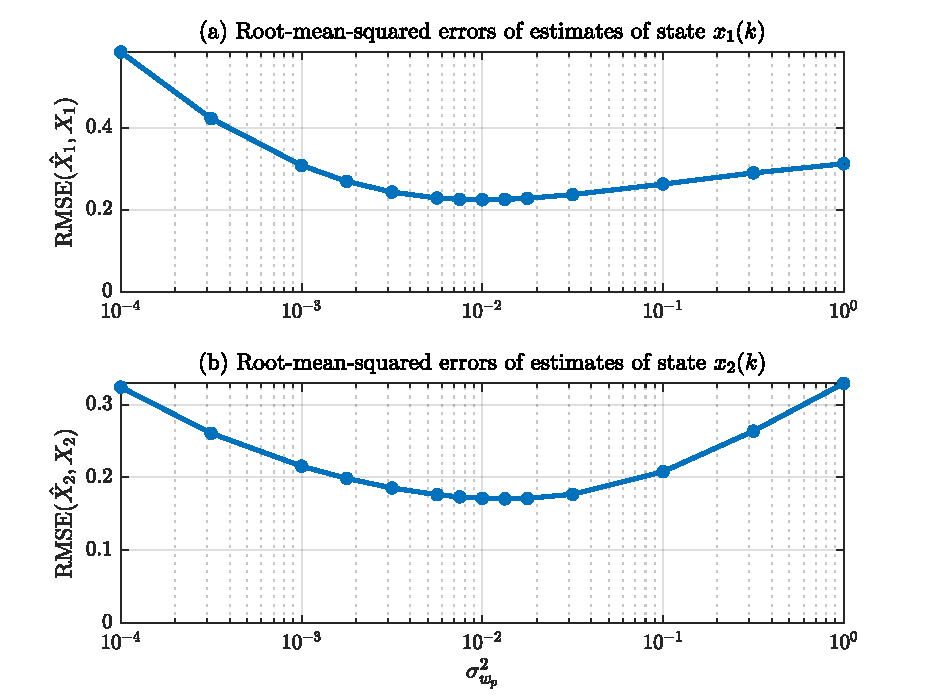
\includegraphics[width=13cm]{images/rod_obs_sim1_3KF_Q_seed_6.pdf}
	\caption{Tuning of Kalman filter KF3 – SISO system}
	\label{fig:sim-sys-siso-KF3-tuning}
\end{figure}
Figure \ref{fig:sim-sys-siso-KF3-tuning} shows the results of these simulations, from which it can be seen that the lowest \gls{RMSE}s of the state estimates were achieved when the variance parameter $\sigma_{w_p}^2$ was close to $0.01$. Using this result, a third Kalman filter labelled `KF3' was designed with the state disturbance covariance matrix 
\begin{equation} \label{eq:sim-sys-siso-KF3-Q}
	\begin{aligned}
		\mathbf{Q}_{\text{KF3}}=\mathbf{Q}_{\text{opt}}=\begin{bmatrix}
			\sigma_{x}^2 & 0 \\
			0 & \sigma_{w_p,\text{opt}}^2 \\
		\end{bmatrix}=\begin{bmatrix}
			0.1^2 & 0 \\
			0 & 0.1^2 \\
		\end{bmatrix}.
	\end{aligned}
\end{equation}

Figure \ref{fig:sim-sys-siso-KF123-est} shows the estimates of the three Kalman filters described above when simulated on the input-output data. The upper plot shows the output estimates and the lower plot shows the estimates of the model state $x_{a,2}(k)$, which corresponds to the estimate of the \gls{RODD}, $p(k)$. As expected, the response of KF1 to the infrequent step disturbances is noticeably slower than that of the other two. The response of KF2 is fast, but it is sensitive to the measurement noise. KF3 is a compromise between the two—a relatively fast response to the infrequent steps and less sensitivity to the measurement noise.
\begin{figure}[htp]
	\centering
	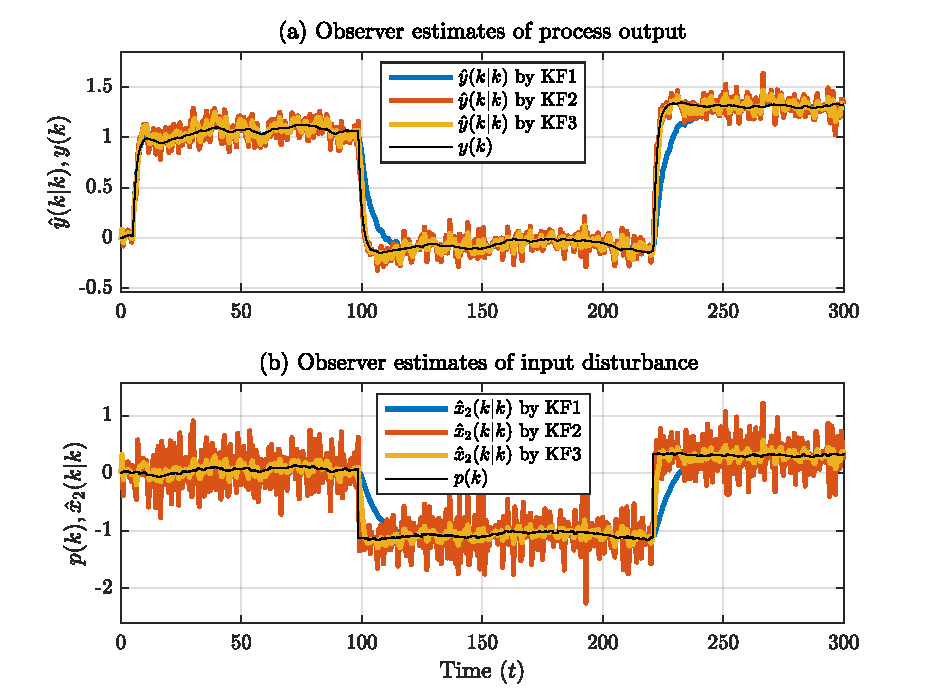
\includegraphics[width=13cm]{images/rod_obs_sim1_all_seed_y_est1_KF123.pdf}
	\caption{Kalman filter estimates}
	\label {fig:sim-sys-siso-KF123-est}
\end{figure}

One way to visualise the observer performance is to plot the square of the output estimation errors, which are the differences between the estimates, $\hat{y}(k \mid k)$, and the true values of the system outputs, $y(k)$. The upper plot in Figure \ref{fig:sim-sys-siso-KF123-cumerr} shows the squared errors in the output estimates of the three Kalman filters. The lower plot shows the cumulative sum of the squared errors. This clearly shows the differences in performance. The estimation errors of KF1 are small when the system is in steady-state but increase dramatically after each step disturbance. The magnitude of the errors of KF2 during steady-state periods is high but roughly constant throughout the simulation. KF3 achieves the lowest overall cumulative sum-of-squared-errors by the end of the simulation.
\begin{figure}[htp]
	\centering
	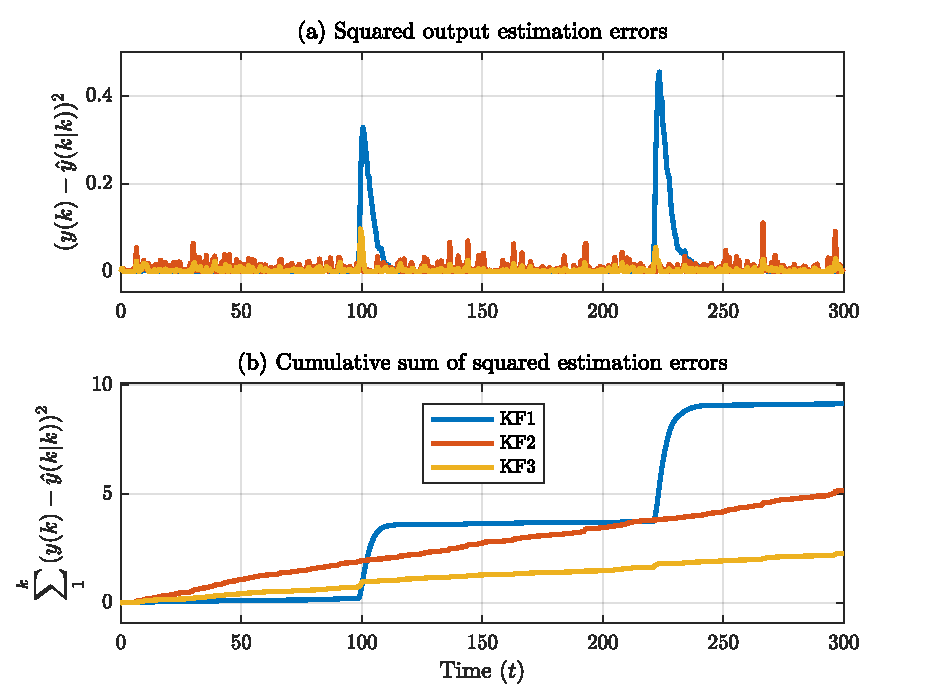
\includegraphics[width=13cm]{images/rod_obs_sim1_all_seed_cum_err_y1_KF123.pdf}
	\caption{Cumulative errors of Kalman filter estimates}
	\label{fig:sim-sys-siso-KF123-cumerr}
\end{figure}

The RMSEs of the state estimates in these simulations are shown in Figure \ref{fig:rod-obs-sim1-KF123-xest-RMSE-bar}. These plots show the total RMSEs divided into two components. The blue part, labelled `no noise' is the RMSE when the system was simulated without measurement noise, (i.e. $y_M(k)=y(k)$). The orange part, labelled `due to noise' represents the difference in the RMSE between simulating with measurement noise and without. This distinction is only possible with a simulation model---in real applications it is not possible to obtain the true system outputs.
\begin{figure}[htp]
	\centering
	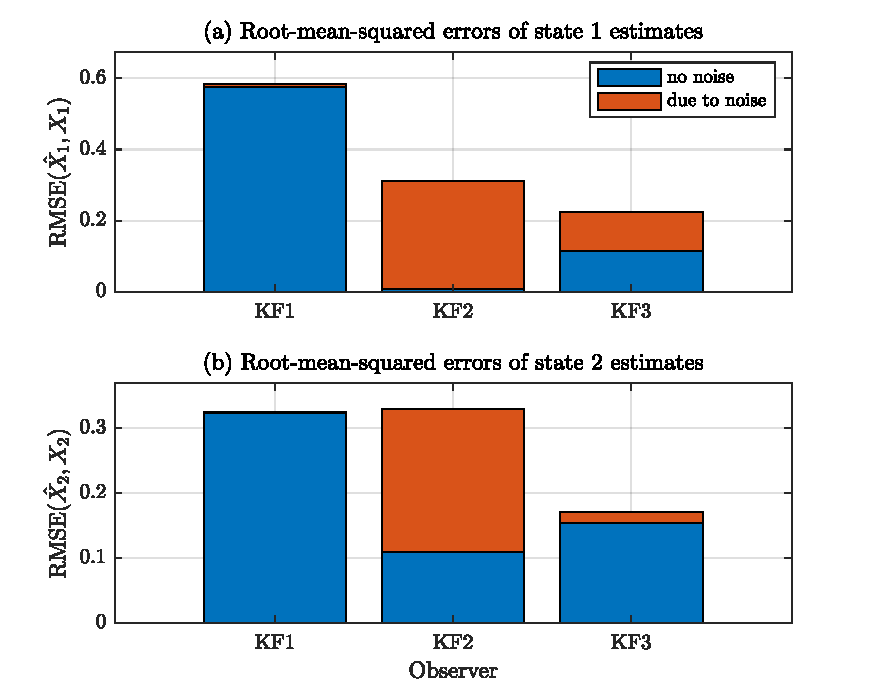
\includegraphics[width=12cm]{images/rod_obs_sim1_all_seed_x_err_bar_KF123.pdf}
	\caption{Root-mean-squared errors of state estimates – SISO system}
	\label{fig:rod-obs-sim1-KF123-xest-RMSE-bar}
\end{figure}

As well as allowing the overall RMSE values of the three Kalman filters to be compared, these plots also illustrate the relative magnitudes of the sources of the error. As expected, the errors of KF1 are almost all due to its slow dynamic response to the shocks, whereas very little is due to the measurement noise. The opposite is true of KF2, which has a very fast dynamic response to the shocks. The trade-off between the two sources of errors is clearly illustrated for KF3. It should be noted that this may not be the best trade-off in every case. In some applications, the speed of response may be more important than the sensitivity to noise, or vice-versa. The trade-off resulting from minimizing the overall RMSE is used in this work.

\subsubsection{Selection of multiple-model observer parameters} \label{sec:sim-obs-lin-1-MKF-tuning}

Parameter values for the sub-optimal multiple-model observer algorithms described in Section \ref{sec:fusion} were chosen by a similar method. The sequence fusion algorithms proposed by \cite{robertson_detection_1995} and \cite{robertson_method_1998} have three parameters, \gls{nf}, \gls{m}, and \gls{d}. Candidate values for these parameters were generated by considering every combination satisfying

\begin{equation} \label{eq:sim-sys-siso-MKF-SF-param-values}
	\begin{aligned}
		\frac{N_f}{N_d} &\in \left\{3, 5, 10, 15, 20\right\},  \\
		n_\text{max} &\in \left\{1, 2, 3\right\},  \\
		N_d &\in \left\{1, 2, 3, 5, 10\right\}.
	\end{aligned}
\end{equation}

Note that $\frac{\gls{nf}}{\gls{d}}$ represents the number of detection intervals within the fusion horizon and is always a whole number. For example, when $\gls{d}=3$, the lengths of the fusion were 9, 15, 30, 45, and 60. However, not all combinations were simulated. Any combination with more than 200 hypotheses ($\gls{nh}>200$) or with a total probability modelled, \gls{beta} (\ref{eq:p_gamma}), less than 0.85 was rejected. The remaining 58 combinations were then evaluated by simulating the observer and calculating the \gls{RMSE} of the output estimates on the 5000 data samples from the simulated system. Tables \ref{tb:obs-sim1-popt-SF95} and \ref{tb:obs-sim1-popt-SF98} show the resulting \gls{RMSE} results for the 10 best combinations of parameter values (those with the lowest output \gls{RMSE}) for the 1995 and 1998 variants of this algorithm.
\begin{table}[ht]
	\begin{center}
		\caption{Multi-model observer parameter search results – MKF--SF95.} \label{tb:obs-sim1-popt-SF95}
		% See: https://texblog.org/2019/06/03/control-the-width-of-table-columns-tabular-in-latex/
		\begin{tabular}{p{0.05\textwidth}>{\centering\arraybackslash}p{0.07\textwidth}>{\centering\arraybackslash}p{0.07\textwidth}>{\centering\arraybackslash}p{0.07\textwidth}>{\centering\arraybackslash}p{0.07\textwidth}>{\centering\arraybackslash}p{0.15\textwidth}}
			\gls{nf} & \gls{m} & \gls{d} & \gls{nh} & \gls{beta} & $\text{\gls{RMSE}}(\hat{Y},Y)$  \\
			\hline
			% See script rod_obs_sim1_MKF_SF95_popt_table.m
			% 29-Nov-2022 18:35:37 results with seed = 6, sigma_M = 0.1, d_min = 1
			15 &   2 &   1 & 151 & 0.9996 & 0.0411 \\
			20 &   2 &   1 & 251 & 0.9990 & 0.0411 \\
			10 &   2 &   1 &  76 & 0.9999 & 0.0411 \\
			10 &   3 &   1 & 268 & 1.0000 & 0.0411 \\
			5 &   1 &   1 &   8 & 0.9990 & 0.0415 \\
			5 &   2 &   1 &  26 & 1.0000 & 0.0415 \\
			5 &   3 &   1 &  48 & 1.0000 & 0.0415 \\
			15 &   1 &   1 &  18 & 0.9904 & 0.0418 \\
			10 &   1 &   1 &  13 & 0.9957 & 0.0419 \\
			10 &   2 &   2 &  16 & 0.9043 & 0.0426 \\
			\hline
		\end{tabular}
	\end{center}
\end{table}
\begin{table}[ht]
	\begin{center}
		\caption{Multi-model observer parameter search results – MKF--SF98.} \label{tb:obs-sim1-popt-SF98}
		% See: https://texblog.org/2019/06/03/control-the-width-of-table-columns-tabular-in-latex/
		\begin{tabular}{p{0.05\textwidth}>{\centering\arraybackslash}p{0.07\textwidth}>{\centering\arraybackslash}p{0.07\textwidth}>{\centering\arraybackslash}p{0.07\textwidth}>{\centering\arraybackslash}p{0.07\textwidth}>{\centering\arraybackslash}p{0.15\textwidth}}
			\gls{nf} & \gls{m} & \gls{d} & \gls{nh} & \gls{beta} & $\text{\gls{RMSE}}(\hat{Y},Y)$  \\
			\hline
			% See script rod_obs_sim1_MKF_SF98_popt_table
			% 29-Nov-2022 18:38:45 results with seed = 6, sigma_M = 0.1, d_min = 1
%			15 &   2 &   1 & 151 & 0.9996 & 0.0411 \\
%			20 &   2 &   1 & 251 & 0.9990 & 0.0411 \\
%			10 &   2 &   1 &  76 & 0.9999 & 0.0411 \\
%			10 &   3 &   1 & 268 & 1.0000 & 0.0411 \\
%			5 &   1 &   1 &   8 & 0.9990 & 0.0415 \\
%			5 &   2 &   1 &  26 & 1.0000 & 0.0415 \\
%			5 &   3 &   1 &  48 & 1.0000 & 0.0415 \\
%			15 &   1 &   1 &  18 & 0.9904 & 0.0418 \\
%			10 &   1 &   1 &  13 & 0.9957 & 0.0419 \\
%			20 &   1 &   1 &  23 & 0.9831 & 0.0429 \\
			% See script rod_obs_sim1_MKF_SF98_popt_table.m
			% 07-Dec-2022 23:56:27 results with seed = 6, sigma_M = 0.1, d_min = 1
			30 &   2 &   2 & 151 & 0.9970 & 0.0414 \\
			20 &   2 &   2 &  76 & 0.9991 & 0.0414 \\
			10 &   2 &   2 &  26 & 0.9999 & 0.0414 \\
			10 &   3 &   2 &  48 & 1.0000 & 0.0414 \\
			6 &   1 &   2 &   6 & 0.9988 & 0.0414 \\
			6 &   2 &   2 &  13 & 1.0000 & 0.0414 \\
			6 &   3 &   2 &  16 & 1.0000 & 0.0414 \\
			10 &   1 &   2 &   8 & 0.9962 & 0.0416 \\
			9 &   1 &   3 &   6 & 0.9974 & 0.0418 \\
			9 &   2 &   3 &  13 & 1.0000 & 0.0418 \\
			\hline
		\end{tabular}
	\end{center}
\end{table}

From a practical standpoint, it is not desirable to simulate a large number of hypotheses. On this basis, the third combination in Table \ref{tb:obs-sim1-popt-SF95} ($\gls{nf}=10,\gls{m}=2,\gls{d}=1$, requiring 76 hypotheses) or the fifth ($\gls{nf}=5,\gls{m}=1,\gls{d}=1$, requiring only 8 hypotheses) are good choices for the 1995 version. The fifth combination was chosen for the simulations and the observer was labelled `MKF--SF95'. 

In terms of overall estimation errors, the two sequence fusion algorithms are very similar. Note that in the case of the 1998 version, it produces identical results to the MKF--SF95 observer when the spacing parameter \gls{d} is 1. The differences between the two algorithms are only in the way the estimates are updated during the steps of the detection interval. Therefore, results for the 1998 algorithm with $\gls{d}=1$ were discarded. \cite{robertson_method_1998} state that the approach is a means of obtaining a long detection horizon, which is necessary when many sampling intervals are required to discriminate among multiple abrupt changes that may occur. Since in this simulation there is only one \gls{RODD} disturbance, and the best results were achieved with a detection interval of 1, it was concluded that these features of the 1998 algorithm were not applicable to this problem.

Nevertheless, based on the results in Table \ref{tb:obs-sim1-popt-SF98}, an observer labelled `MKF--SF1' was selected for simulation with $\gls{nf}=6$, $\gls{m}=1$, and $\gls{d}=2$. This requires only 6 hypotheses and achieves as good a performance as `MKF--SF95'.

The sequence pruning algorithm proposed by \cite{eriksson_classification_1996} has two parameters that must be specified, \gls{nh}, and \gls{nmin}. Candidate values for these parameters were generated by considering all combinations satisfying

\begin{equation} \label{eq:sim-sys-siso-MKF-SP-param-values}
	\begin{aligned}
		\gls{nh} &\in \left\{3, 4, 5, 7, 10, 14, 19, 25, 32\right\},  \\
		\gls{nmin} &\in \left\{1, 2, 3, 4, 5, 6, 7, 9, 12, 16, 21\right\}.
	\end{aligned}
\end{equation}

Combinations where rejected when $\gls{nh} - \gls{nmin} < 1$, or in other words, when the minimum life, \gls{nmin}, was greater than or equal to the number of hypotheses, \gls{nh}. This is a necessary condition since there must be enough filters to simulate the hypotheses until they reach the minimum life. Each remaining combination was then evaluated in the same way by calculating the \gls{RMSE} of the output estimates on the same 5000 samples used in the tuning of the sequence fusion observers described above. Table \ref{tb:obs-sim1-popt-SP} shows the top 10 combinations of parameter values in terms of lowest \gls{RMSE}.

\begin{table}[ht]
	\begin{center}
		\caption{Multi-model observer parameter search results – MKF--SP.} \label{tb:obs-sim1-popt-SP}
		% See: https://texblog.org/2019/06/03/control-the-width-of-table-columns-tabular-in-latex/
		\begin{tabular}{p{0.05\textwidth}>{\centering\arraybackslash}p{0.07\textwidth}>{\centering\arraybackslash}p{0.15\textwidth}}
			\gls{nh} & \gls{nmin} & $\text{\gls{RMSE}}(\hat{Y},Y)$  \\
			\hline
			% See script rod_obs_sim1_MKF_SP_popt_table.m
			% 29-Nov-2022 18:24:40 results with seed = 6, sigma_M = 0.1
			10 &   7 & 0.0409  \\
			10 &   6 & 0.0410  \\
			19 &  16 & 0.0411  \\
			14 &  12 & 0.0411  \\
			25 &  21 & 0.0411  \\
			14 &   7 & 0.0411  \\
			19 &   7 & 0.0412  \\
			19 &   6 & 0.0412  \\
			25 &  16 & 0.0412  \\
			25 &  12 & 0.0412  \\
			\hline
		\end{tabular}
	\end{center}
\end{table}

As above, the differences between the \gls{RMSE}s of the best 10 combinations are small, indicating that the choice of parameters from these combinations is not critical. The first combination ($\gls{nh}=10,\gls{nmin}=7$) was chosen and the observer was labelled `MKF--SP1' in the simulations below. Table \ref{tb:obs-params-sim1} is a summary of the parameters of the observers simulated.
\begin{table}[ht]
	\begin{center}
		\caption{Observer parameters for SISO linear system.} \label{tb:obs-params-sim1}
		% See: https://texblog.org/2019/06/03/control-the-width-of-table-columns-tabular-in-latex/
		\begin{tabular}{p{0.16\textwidth}>{\centering\arraybackslash}p{0.12\textwidth}>{\centering\arraybackslash}p{0.16\textwidth}>{\centering\arraybackslash}p{0.16\textwidth}>{\centering\arraybackslash}p{0.16\textwidth}}
			& KF3 & MKF--SF95 & MKF--SF1 & MKF--SP \\
			\hline
			Type & Kalman filter & Multi-model Kalman filter & Multi-model Kalman filter & Multi-model Kalman filter \\
			Algorithm & - & Sequence fusion 95 & Sequence fusion 98 & Sequence pruning \\
			\hline
			Parameters &  &  &  &  \\
			\gls{Qset} & $\mathbf{Q}_{opt}$ & $\{\mathbf{Q}_0,\mathbf{Q}_1\}$ & $\{\mathbf{Q}_0,\mathbf{Q}_1\}$ & $\{\mathbf{Q}_0,\mathbf{Q}_1\}$ \\
			\gls{R} & $0.1^2$ & $0.1^2$ & $0.1^2$ & $0.1^2$ \\
			$\mathbf{P}(0)$ & $\mathbf{P}_0$ & $\mathbf{P}_0$ & $\mathbf{P}_0$ & $\mathbf{P}_0$ \\
			\gls{nh} & 1 & 8 & 6 & 10 \\
			\gls{nf} & - & 5 & 6 & - \\
			\gls{m} & - & 1 & 1 & - \\
			\gls{d} & - & 1 & 2 & - \\
			\gls{nmin} & - & - & - & 7 \\
			\gls{epsilon} & - & 0.01 & 0.01 & 0.01 \\
			\gls{sigmawp} & - & 0.01 & 0.01 & 0.01 \\
			\gls{b} & - & 100 & 100 & 100 \\
			\hline
		\end{tabular}
	\end{center}
\end{table}

\subsubsection{Scheduled Kalman filter} \label{sim-obs-lin-1-SKF}

To determine the best performance that could be achieved by an ideal multiple-model observer, a hypothetical observer that has access to the true shock indicator signal, \gls{gammak}, was simulated. This `scheduled' Kalman filter, labelled ‘SKF’, has only one shock sequence---the correct one---and therefore the process noise covariance is automatically switched to match the known shock signal. The SKF is hypothetical because it could not be implemented in a real application where the random shocks are not known.

\subsubsection{Simulation results} \label{sim-obs-lin-1-results}

Figure \ref{fig:rod-obs-sim1-yest-1-SF} shows the estimates of the sequence fusion observers, MKF--SF95 and MKF--SF1, compared to the scheduled Kalman Filter, SKF, over the first 600 time steps of the simulation. From these results it is apparent that the estimates of the sequence fusion observers are generally very close to those of the SKF. The estimates respond quickly when the random shocks occur and their variance at other times is relatively small despite the measurement noise. A few spontaneous errors of short duration are also noticeable in both the SKF and MKF--SF1 estimates at certain times. However, when the variances are compared to those of the Kalman filters in Figure \ref{fig:sim-sys-siso-KF123-est}, it is clear that these multiple-model observers have an advantage.
\begin{figure}[htp]
	\centering
	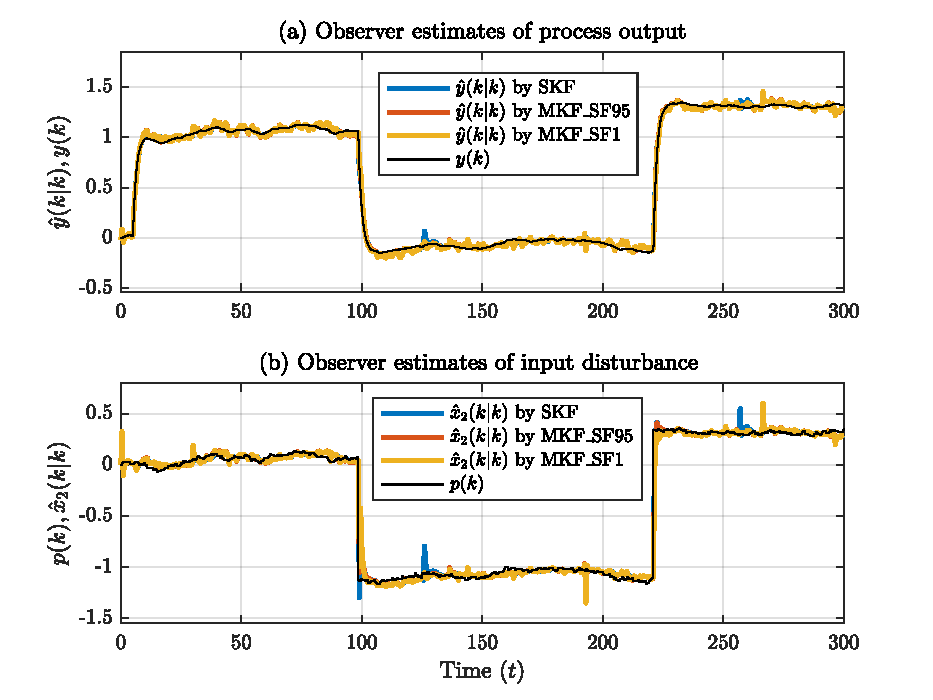
\includegraphics[width=13cm]{images/rod_obs_sim1_all_seed_y_est1_SF95_SF1.pdf}
	\caption{Estimates by sequence fusion observers – SISO system}
	\label{fig:rod-obs-sim1-yest-1-SF}
\end{figure}

Figure \ref{fig:rod-obs-sim1-yest-1-SP} shows the estimates of the sequence pruning observer, MKF--SP1, compared to the scheduled Kalman Filter. It also responds quickly to the shocks and is insensitive to the measurement noise, similar to the sequence fusion observers.
\begin{figure}[htp]
	\centering
	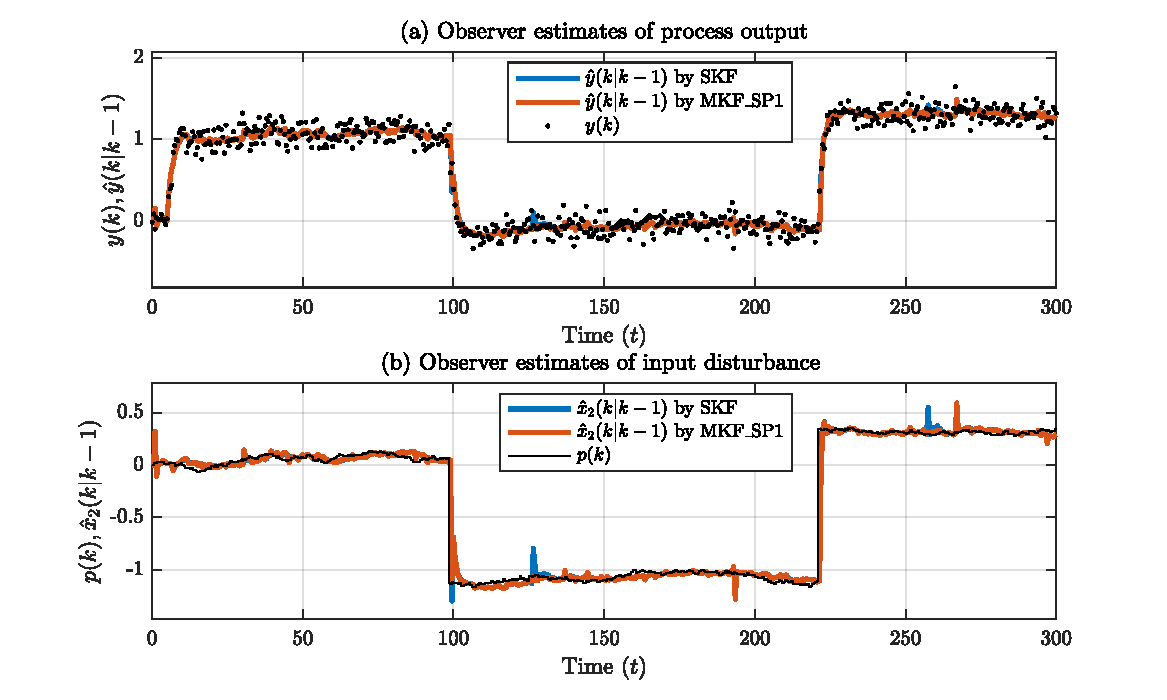
\includegraphics[width=13cm]{images/rod_obs_sim1_all_seed_y_est1_SP1.pdf}
	\caption{Estimates by sequence pruning observer – SISO system}
	\label{fig:rod-obs-sim1-yest-1-SP}
\end{figure}

The plots in Figure \ref{fig:rod-obs-sim1-cum-err-y1-all} show the squared output errors and the cumulative squared-errors of the five observers over the full duration of the simulation. The differences between the multiple-model observers are almost indistinguishable. By the end of the simulation, the cumulative errors are significantly lower than those of KF3 and slightly higher than the SKF.
\begin{figure}[htp]
	\centering
	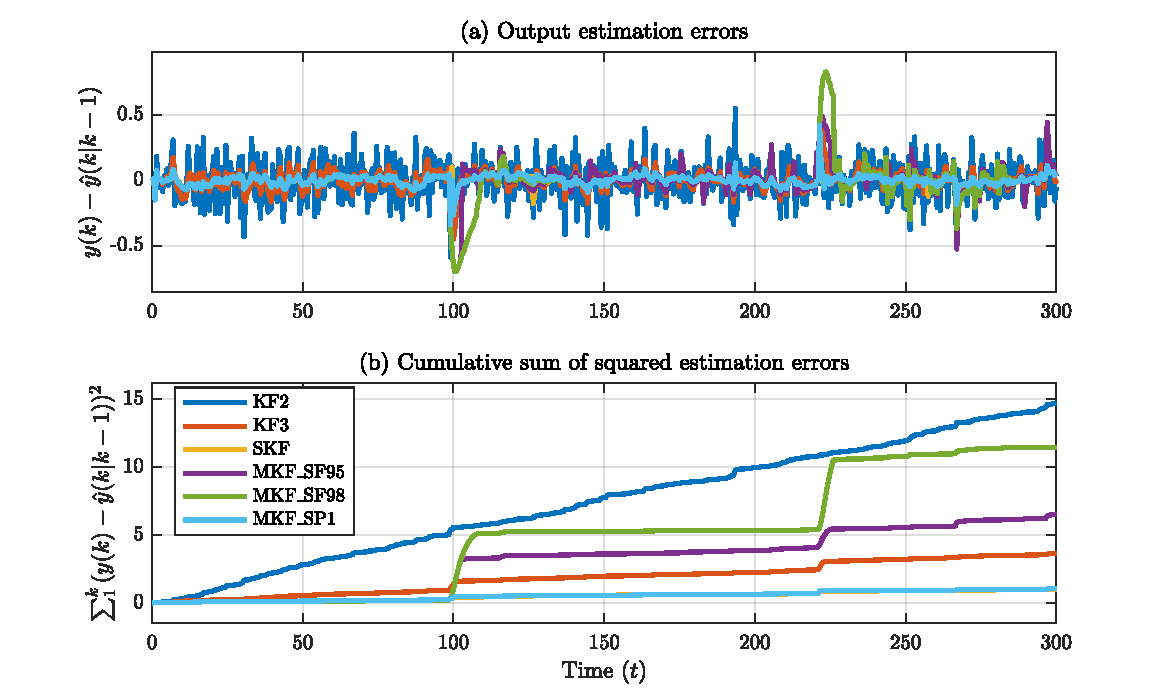
\includegraphics[width=13cm]{images/rod_obs_sim1_all_seed_cum_err_y1.pdf}
	\caption{Cumulative errors of observer estimates – SISO system}
	\label{fig:rod-obs-sim1-cum-err-y1-all}
\end{figure}

Figure \ref{fig:rod-obs-sim1-xest-RMSE-bar} compares the \gls{RMSE}s of the state estimates of the five observers over the full simulation. From this, it can be seen that the multiple-model observers achieve lower RMSEs than KF3, both in simulations with and without noise. The reduction in the errors due to the lower sensitivity to measurement noise (orange bars) is a more significant contribution to the improved performance of the multiple-model observers. It is noteworthy that most of the errors in the estimates of state 2, which corresponds to the input disturbance, are not due to measurement noise. This may partly be attributed to the delay in the process, which makes it impossible for the observers to immediately detect an unmeasured disturbance. They are also due to errors in tracking the persistent component of the disturbance, which can be seen in Figures \ref{fig:rod-obs-sim1-yest-1-SF} and \ref{fig:rod-obs-sim1-yest-1-SP}.
\begin{figure}[htp]
	\centering
	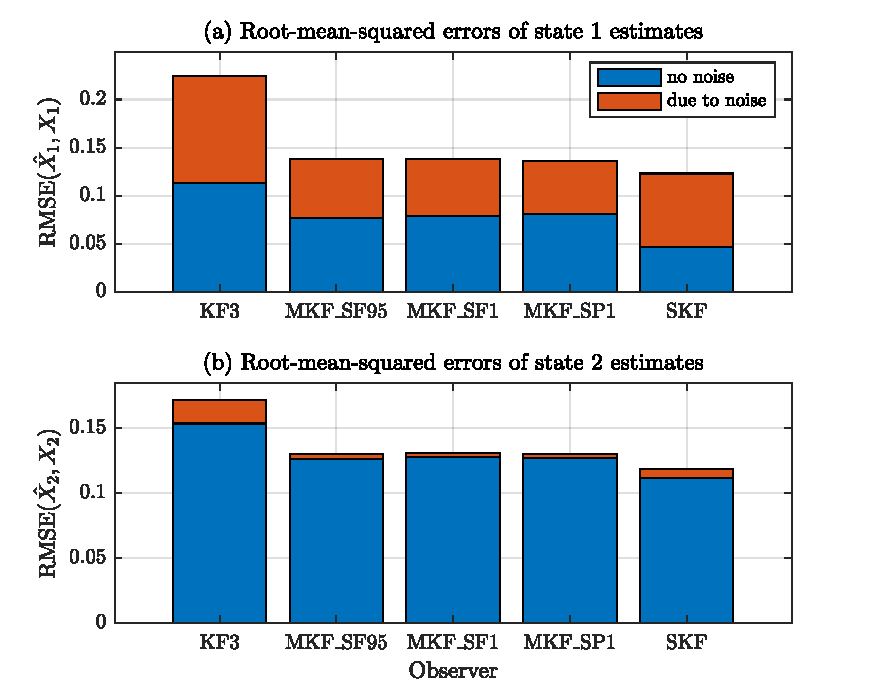
\includegraphics[width=12cm]{images/rod_obs_sim1_all_seed_x_err_bar.pdf}
	\caption{Root-mean-squared errors of state estimates – SISO system}
	\label{fig:rod-obs-sim1-xest-RMSE-bar}
\end{figure}

Because these processes are stochastic, it is important to run simulations of sufficient duration to be confident that the results are representative of average performance. Figure \ref{fig:rod-obs-sim1-yest-all-seed-RMSE-box} provides an indication of the sensitivity of the \gls{RMSE} results to the initialization of the pseudo-random number generator used in these simulations. The data for this figure are from the results of 10 simulations, each of 5000 samples and each with a different pseudo-random initialization. It can be seen that the \gls{RMSE} values are somewhat sensitive to the random initialization but the variation is an order of magnitude lower than the difference between the multiple-model observers and KF3.
\begin{figure}[htp]
	\centering
	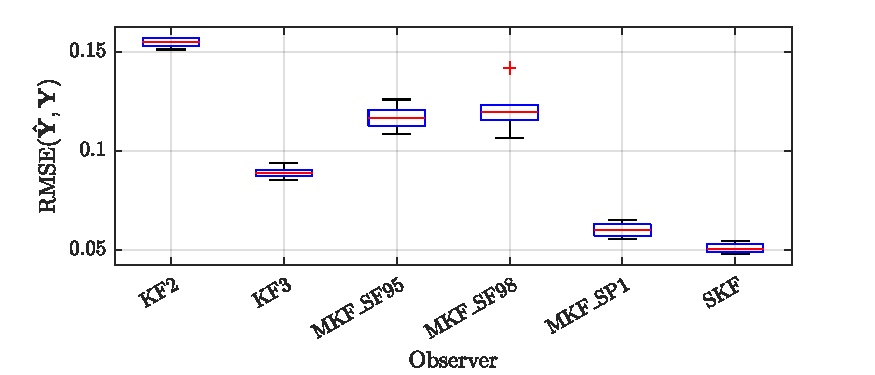
\includegraphics[width=12cm]{images/rod_obs_sim1_all_seed_y_err_box.pdf}
	\caption{Sensitivity of output estimation errors to random initialization – SISO system}
	\label{fig:rod-obs-sim1-yest-all-seed-RMSE-box}
\end{figure}
Figure \ref{fig:rod-obs-sim1-yest-all-seed-RMSE-box} confirms that the multiple-model observers are a significant improvement on the best single Kalman filter. However, there is no significant difference between the \gls{MKF}s in this case.
% Plots for analysis of SF performance
%
%\begin{figure}[htp]
%	\centering
%	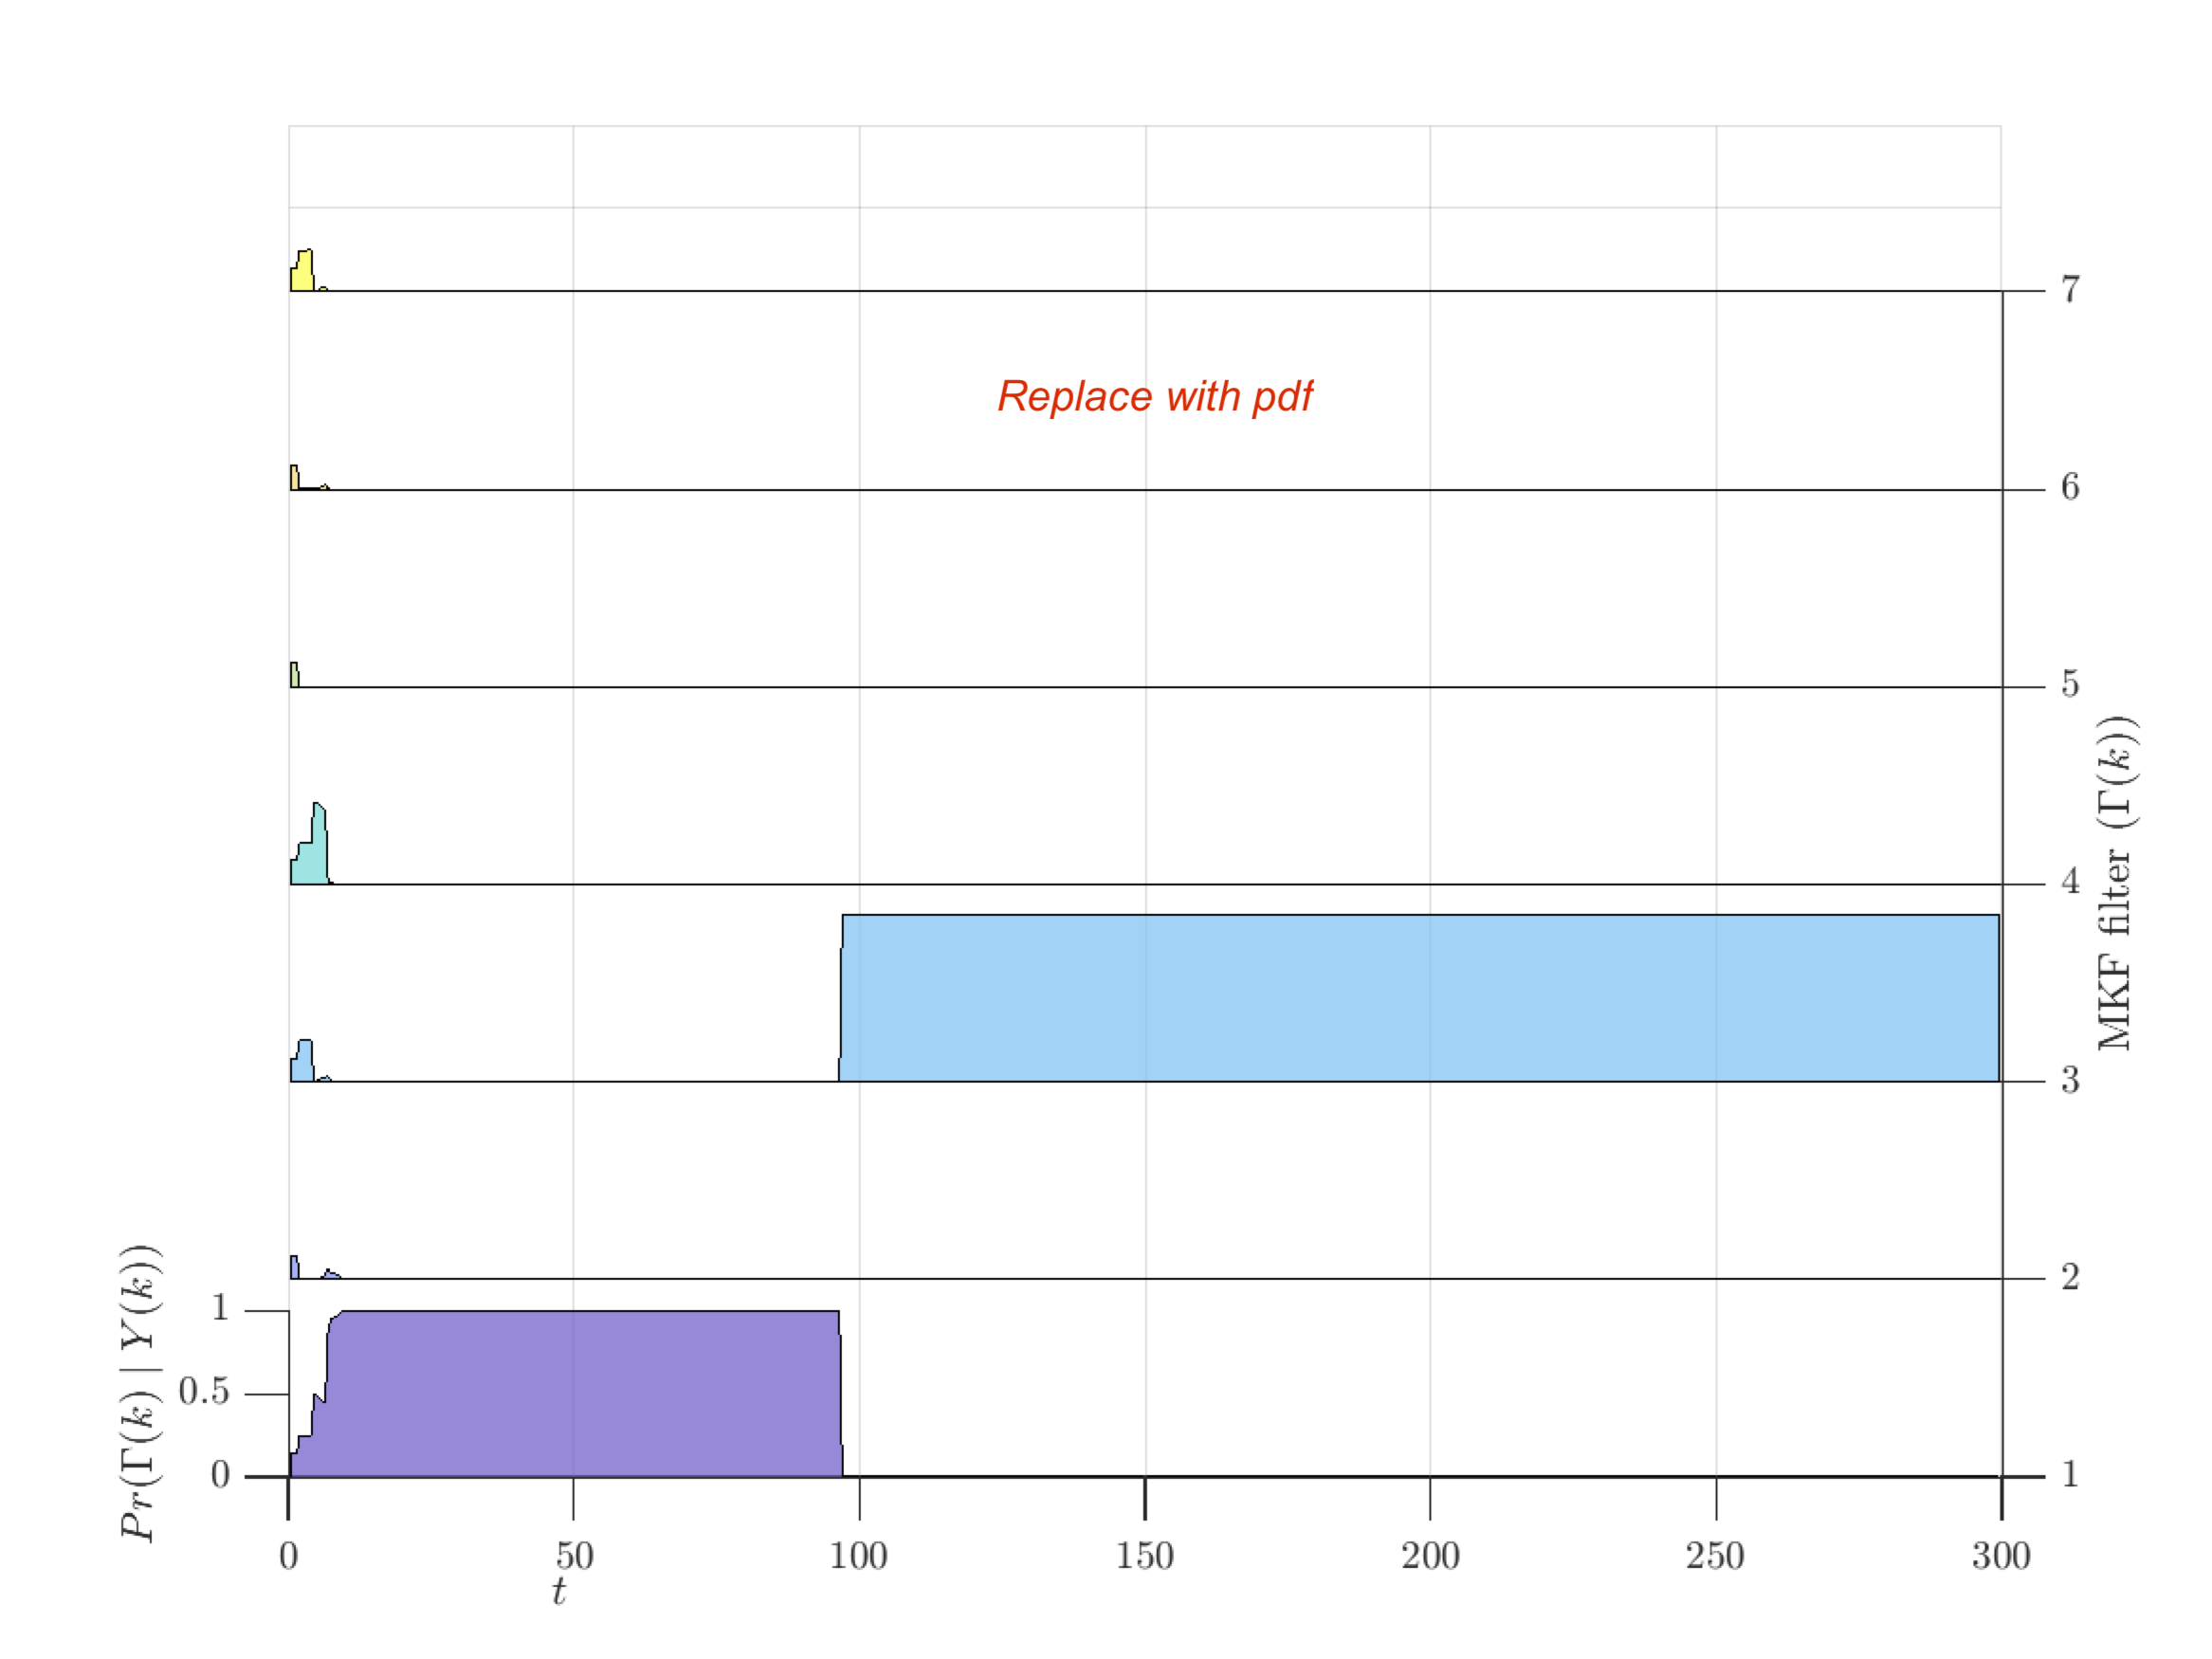
\includegraphics[width=15cm]{images/rod-obs-sim-1-4-wfplot-DRAFT.png}
%	\caption{Evolution of conditional probabilities with sequence fusion}
%	\label{fig:rod-obs-sim1-4-wfplot}
%\end{figure}
%
%\begin{figure}[htp]
%	\centering
%	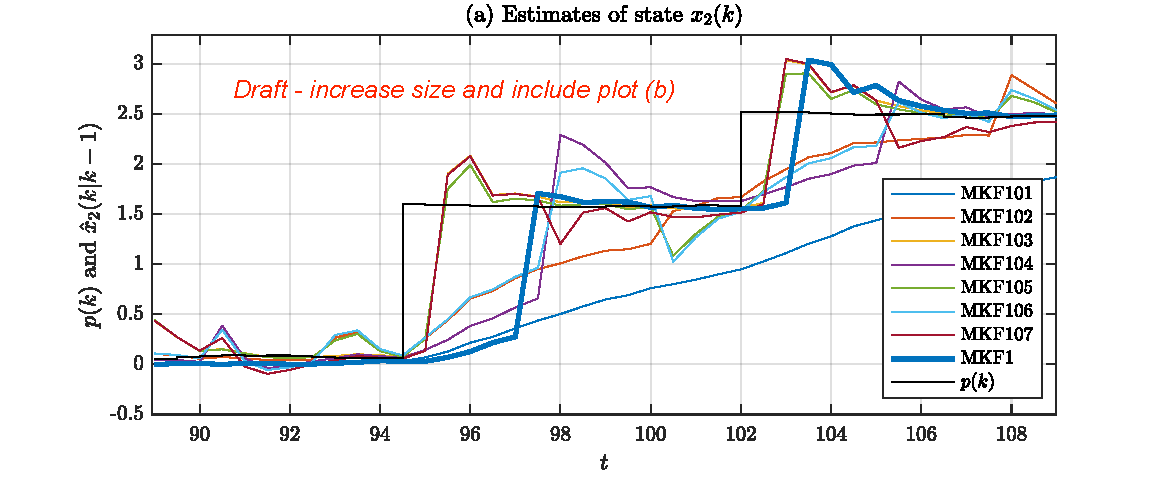
\includegraphics[width=14cm]{images/rod-obs-sim-1-4-est-MKF-SF-plot-DRAFT.pdf}
%	\caption{Filter estimates of sequence fusion observer during step disturbances}
%	\label{fig:rod-obs-sim1-4-est-MKF-SF-plot-DRAFT}
%\end{figure}
%
%\begin{figure}[htp]
%	\centering
%	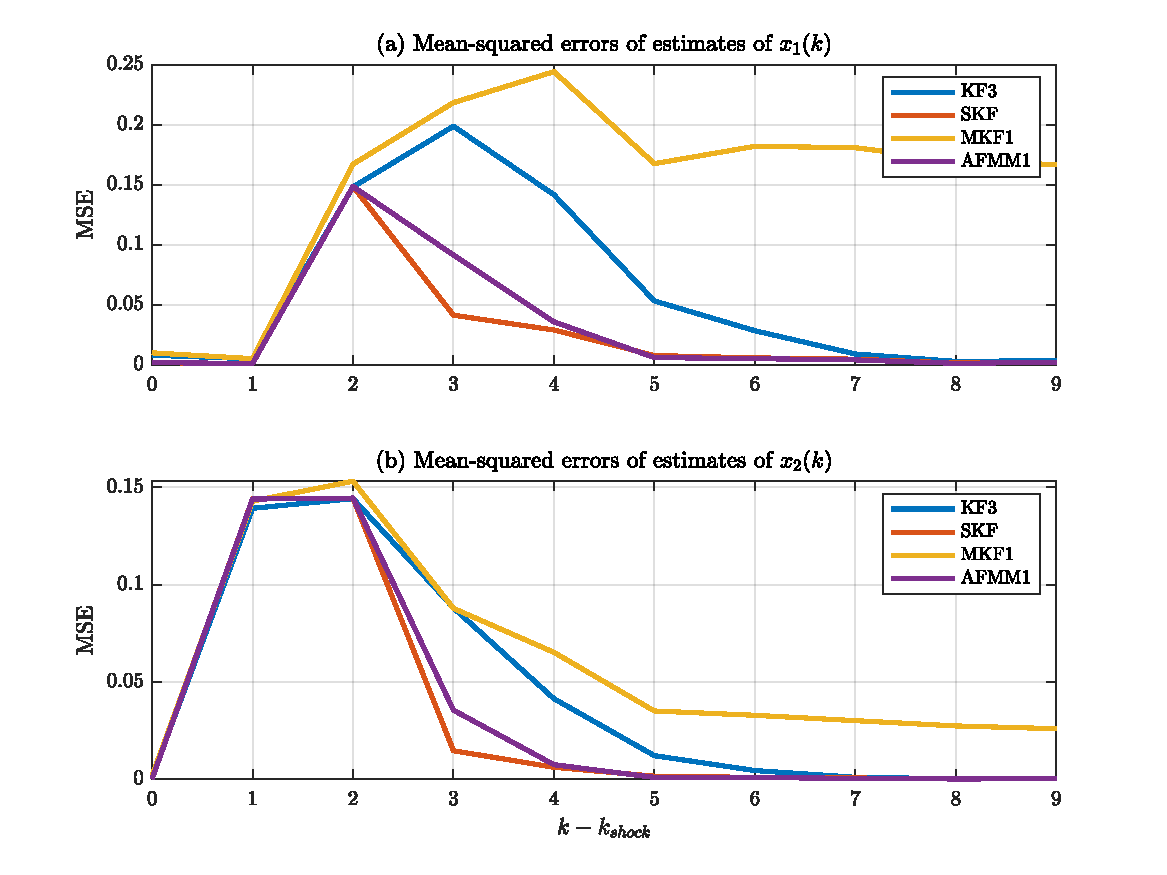
\includegraphics[width=14cm]{images/rod_obs_sim2_7_mse_ashocks.pdf}
%	\caption{Average errors of observer estimates after shock disturbances}
%	\label{fig:rod_obs_sim2_7_mse_ashocks}
%\end{figure}

\subsection{MIMO linear system} \label{sim-obs-lin-2}

\cite{robertson_method_1998} stated that in the case of more than one \gls{RODD} disturbance, it often takes many sampling intervals to discriminate among possible disturbances. The main motivation for the detection intervals used in their approach was to achieve a longer \textit{detection horizon} without requiring a very large number of hypotheses. To evaluate this feature, a \textit{multiple-input, multiple-output} (\gls{MIMO}) system with a 2-input, 2-output ($2\times2$) process model was chosen. The system has two independent \gls{RODD} step disturbances added to each manipulated input, as shown in the functional diagram in Figure \ref{fig:sim-sys-diag-2x2}. 
\begin{figure}[htp]
	\centering
	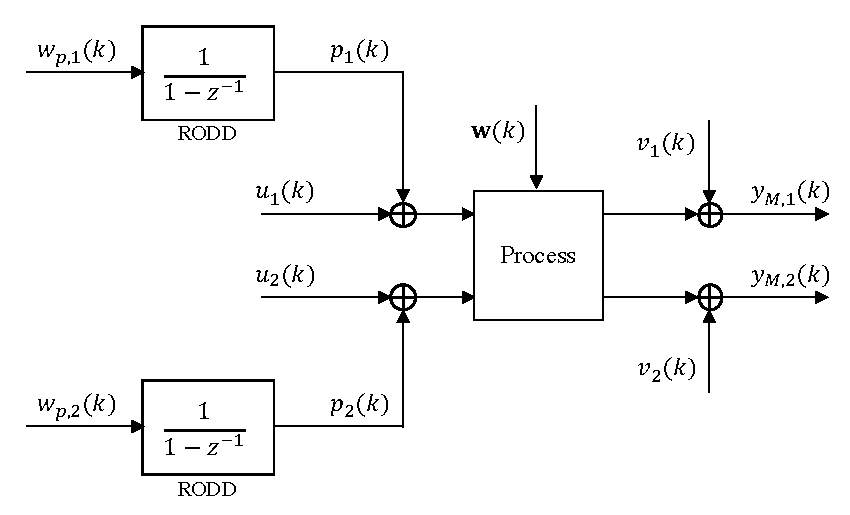
\includegraphics[width=11.5cm]{images/sim-sys-diag-2x2.pdf}
	\caption{Functional diagram of the simulated MIMO system}
	\label{fig:sim-sys-diag-2x2}
\end{figure}

The process model is a discrete-time linear model derived from the $2\times2$ continuous-time system,
% 2x2 system #1 - see sys_rodin_step_2x2sym.m
%\begin{equation} \label{eq:sim-sys-mimo-ct}
%	\mathbf{G}(s) = \left[\begin{array}{cc}
%		G_{11}(s) & G_{12}(s)  \\
%		G_{21}(s) & G_{22}(s)  \\
%	\end{array}\right] = \left[\begin{array}{cc}
%		\frac{1}{1+8.5s} & \frac{-0.5}{1+8.5s}  \\
%		\frac{-0.5}{1+8.5s} & \frac{1}{1+8.5s}  \\
%	\end{array}\right]
%\end{equation}
% 2x2 system #2 - see sys_rodin_step_2x2sym2.m
\begin{equation} \label{eq:sim-sys-mimo-ct}
	\mathbf{G}(s) = \left[\begin{array}{cc}
		G_{11}(s) & G_{12}(s)  \\
		G_{21}(s) & G_{22}(s)  \\
	\end{array}\right] = \left[\begin{array}{cc}
		\frac{1}{1+8.5s} & \frac{0.5}{1+8.5s}  \\
		\frac{0.5}{1+8.5s} & \frac{1}{1+8.5s}  \\
	\end{array}\right],
\end{equation}
where $s$ is the Laplace variable.  This model was chosen because the dynamics of each input-output combination are similar (they have the same time constant and the sign of the gain is the same). The only differences are in the magnitude of the static gains. The model was converted to a discrete-time model with a sampling period of one ($\gls{Ts}=1$). The discrete-time state space model of the augmented system used by the observers was
\begin{equation} \label{eq:sim-sys-2x2-ss-aug}
	\begin{split}
		\mathbf{x}_{a}(k+1) & =\left[\begin{array}{cccc}
			0.8890 & 0 & 1 & 0.5 \\
			0 & 0.8890 & 0.5 & 1 \\
			0 & 0 & 1 & 0 \\
			0 & 0 & 0 & 1
		\end{array}\right] \mathbf{x}_{a}(k) + \left[\begin{array}{cc}
			1 & 0.5 \\
			0.5 & 1
		\end{array}\right] \mathbf{u}(k) + \mathbf{w}_{a}(k) \\
		y(k) & =\left[\begin{array}{cccc}
			0.1110 & 0 & 0 & 0 \\
			0 & 0.1110 & 0 & 0
		\end{array}\right] \mathbf{x}_{a}(k) + v(k)
	\end{split}
\end{equation}
where
\begin{equation} \label{eq:sim-sys-2x2-ss-aug2}
	\mathbf{x}_{a}(k) = \left[\begin{array}{l}
		x_{1}(k) \\
		x_{2}(k) \\
		p_{1}(k) \\
		p_{2}(k)
	\end{array}\right], \mathbf{w}_{a}(k) = \left[\begin{array}{l}
		w_1(k) \\
		w_2(k) \\
		w_{p,1}(k) \\
		w_{p,2}(k)
	\end{array}\right].
\end{equation}

Note that with this representation, the third and fourth model states, $x_{a,3}(k)$ and $x_{a,4}(k)$, correspond exactly to the two input disturbances, $p_1(k)$ and $p_2(k)$.

The two random shocks were simulated with the same parameters as those in the \gls{SISO} simulation, $\epsilon_i=0.01, \sigma_{w_{p,i}}=0.01$, and $b_i=100$. However, the standard deviations of the measurement noises, $\sigma_{M,1}$ and $\sigma_{M,2}$, were 0.2, which is twice as high as they were in the \gls{SISO} simulations.

Figure \ref{fig:rod-obs-sim-2-ioplot} shows the first 300 input-output samples from a simulation of the system with a total duration of 5000. The lower of the two plots shows the input signals, $u_1(k)$, $u_2(k)$, $p_1(k)$, and $p_2(k)$. In this simulation, there were no changes to the known input variables. The upper plot shows the simulated output measurements, $y_1(k)$ and $y_2(k)$. No input disturbances other than $w_{p,1}(k)$ and $w_{p,2}(k)$ were simulated (i.e. $w_1(k)=w_2(k)=0$).
\begin{figure}[htp]
	\centering
	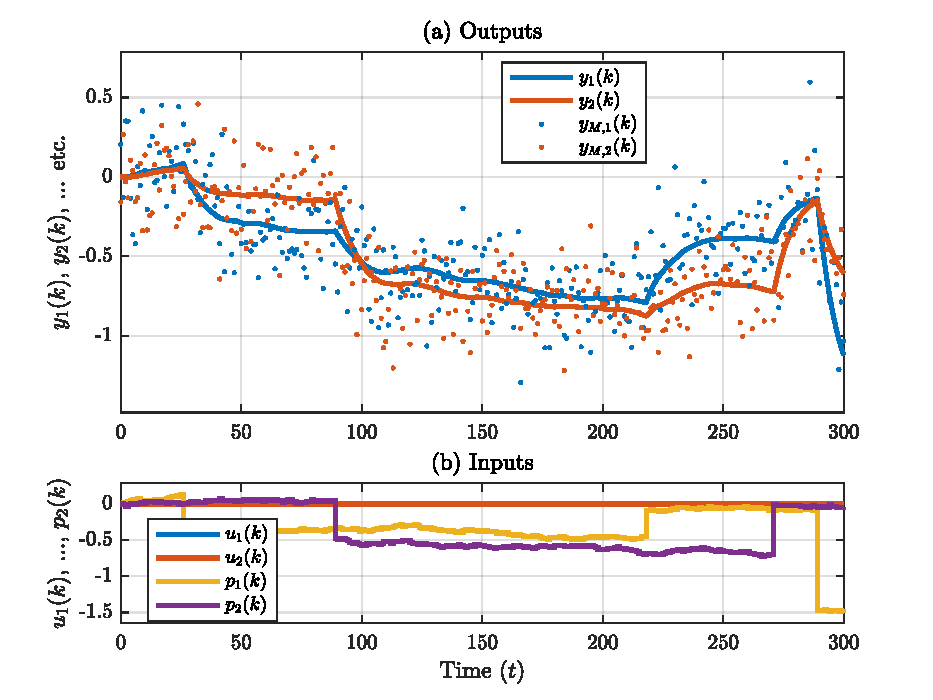
\includegraphics[width=13cm]{images/rod_obs_sim3_all_seed_ioplot.pdf}
	\caption{Simulation of linear MIMO system with two \gls{RODD}s}
	\label{fig:rod-obs-sim-2-ioplot}
\end{figure}

As in the previous experiment, a standard Kalman filter was tuned experimentally to achieve a low \gls{RMSE} of the output estimates. The details of this tuning process are included in Annex \ref{sec:annex-sim-2-KF-tuning} including the resulting value of $\mathbf{Q}_{\text{KF3}}$ (\ref{eq:sim-sys-sim3-KF3-Q}).


\subsubsection{Selection of multiple-model observer parameters}

Parameter values for the sub-optimal multiple-model observers were chosen by a similar method to that used in the SISO experiment. The details of the parameter search and selection process are in Annex \ref{sec:annex-sim-2-MKF-tuning}. Table \ref{tb:obs-params-sim2} summarises the observer parameters used in the simulations.
\begin{table}[ht]
	\begin{center}
		\caption{Observer parameters for MIMO linear system.} \label{tb:obs-params-sim2}
		% See: https://texblog.org/2019/06/03/control-the-width-of-table-columns-tabular-in-latex/
		\begin{tabular}{p{0.16\textwidth}>{\centering\arraybackslash}p{0.12\textwidth}>{\centering\arraybackslash}p{0.16\textwidth}>{\centering\arraybackslash}p{0.16\textwidth}>{\centering\arraybackslash}p{0.16\textwidth}}
			& KF3 & MKF--SF95 & MKF--SF1 & MKF--SP1 \\
			\hline
			Type & Kalman filter & Multi-model Kalman filter & Multi-model Kalman filter & Multi-model Kalman filter \\
			Algorithm & - & Sequence fusion 95 & Sequence fusion 98 & Sequence pruning \\
			\hline
			Parameters &  &  & &  \\
			\gls{Qset} & $\mathbf{Q}_{opt}$ & $\{\mathbf{Q}_0,\mathbf{Q}_1\}$ & $\{\mathbf{Q}_0,\mathbf{Q}_1\}$ & $\{\mathbf{Q}_0,\mathbf{Q}_1\}$ \\
			\gls{R} & $\left[\begin{smallmatrix}0.2^2 & 0 \\ 0 & 0.2^2\end{smallmatrix}\right]$
			& $\left[\begin{smallmatrix}0.2^2 & 0 \\ 0 & 0.2^2\end{smallmatrix}\right]$
			& $\left[\begin{smallmatrix}0.2^2 & 0 \\ 0 & 0.2^2\end{smallmatrix}\right]$
			& $\left[\begin{smallmatrix}0.2^2 & 0 \\ 0 & 0.2^2\end{smallmatrix}\right]$ \\
			$\mathbf{P}(0)$ & $\mathbf{P}_0$ & $\mathbf{P}_0$ & $\mathbf{P}_0$ & $\mathbf{P}_0$ \\
			\gls{nh} & 1 & 116 & 58 & 46 \\
			\gls{nf} & - & 15 & 15 & - \\
			\gls{m} & - & 2 & 2 & - \\
			\gls{d} & - & 3 & 5 & - \\
			\gls{nmin} & - & - & - & 21 \\
			\gls{epsilon} & - & $\begin{bsmallmatrix}0.01 & 0.01\end{bsmallmatrix}^\intercal$
			& $\begin{bsmallmatrix}0.01 & 0.01\end{bsmallmatrix}^\intercal$ 
			& $\begin{bsmallmatrix}0.01 & 0.01\end{bsmallmatrix}^\intercal$ \\
			\gls{sigmawp} & - & $\begin{bsmallmatrix}0.01 & 0.01\end{bsmallmatrix}^\intercal$
			& $\begin{bsmallmatrix}0.01 & 0.01\end{bsmallmatrix}^\intercal$ 
			& $\begin{bsmallmatrix}0.01 & 0.01\end{bsmallmatrix}^\intercal$ \\
			\gls{b} & - & $\begin{bsmallmatrix}100 & 100\end{bsmallmatrix}^\intercal$
			& $\begin{bsmallmatrix}100 & 100\end{bsmallmatrix}^\intercal$ 
			& $\begin{bsmallmatrix}100 & 100\end{bsmallmatrix}^\intercal$ \\
			\hline
		\end{tabular}
	\end{center}
\end{table}

\subsubsection{Simulation Results}

Figure \ref{fig:rod-obs-sim2-yest-1-SF} shows the estimates of both sequence fusion observers (MKF--SF95 and MKF--SF1) compared to the scheduled Kalman Filter (SKF) over the first 300 time steps of the simulation. The upper two plots show the estimates of outputs 1 and 2 compared to the true system outputs. The lower two plots show the estimates of states 3 and 4, which correspond to the input disturbances. The largest errors occur in the periods following the shocks. At these times, the estimates of MKF--SF95 and MKF--SF1 lag those of the SKF. At other times, the estimates of all three observers are quite similar. There is no noticeable difference between MKF--SF95 and MKF--SF1.
\begin{figure}[htp]
	\centering
	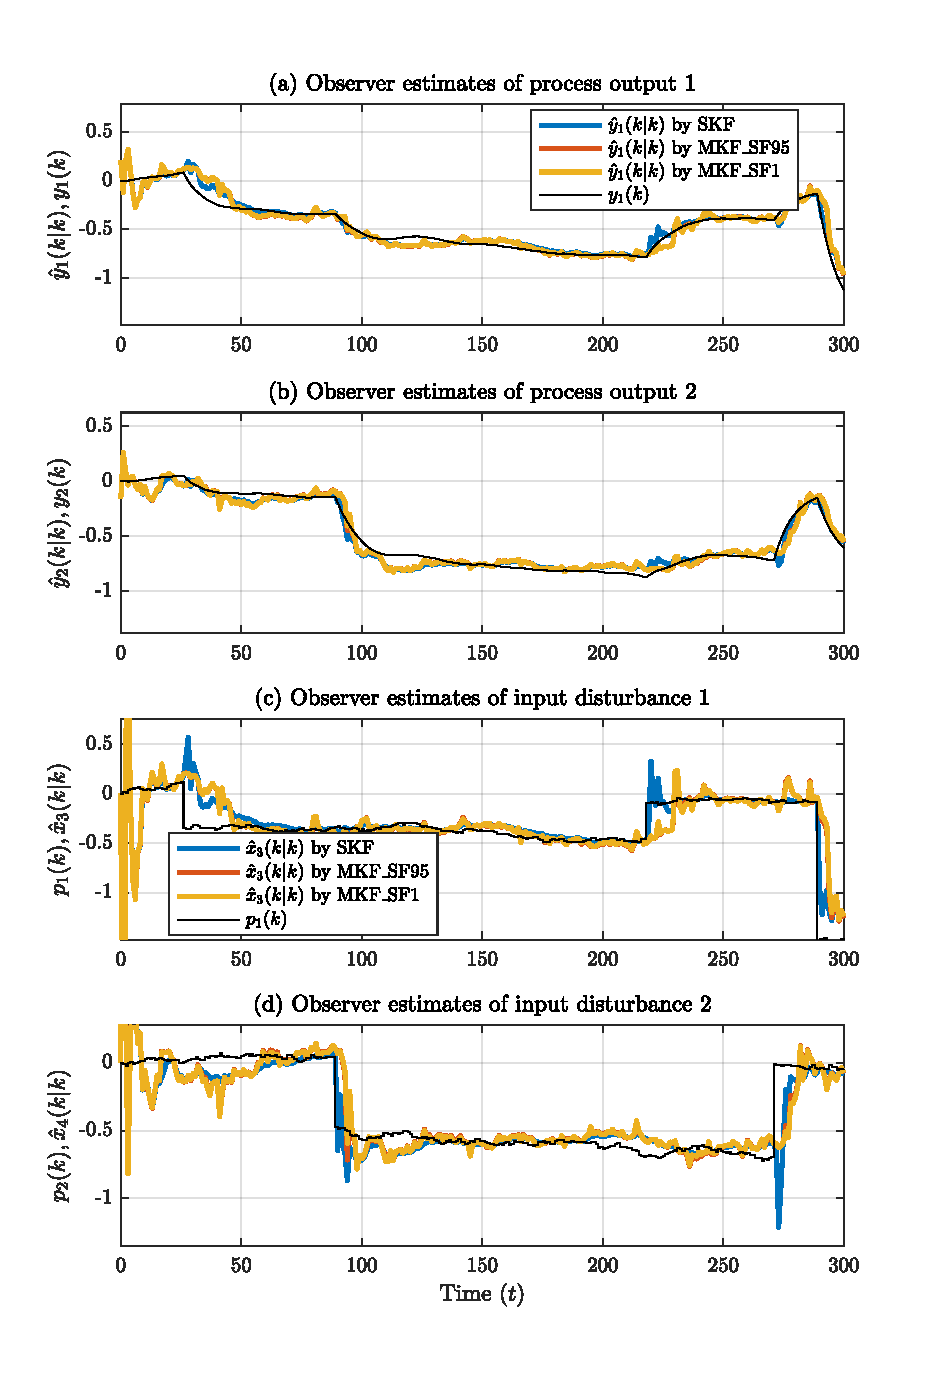
\includegraphics[width=13cm]{images/rod_obs_sim3_all_seed_y_est1_SF95_SF1.pdf}
	\caption{Estimates by sequence fusion observer –  $2\times2$ system}
	\label{fig:rod-obs-sim2-yest-1-SF}
\end{figure}

Figure \ref{fig:rod-obs-sim2-yest-1-SP} shows the estimates of the sequence pruning observer (MKF--SP) compared to the scheduled Kalman Filter on the same simulation data. The behaviour is similar to that of the sequence fusion observers, matching the SKF during periods between shocks and lagging it in the periods immediately after.
\begin{figure}[htp]
	\centering
	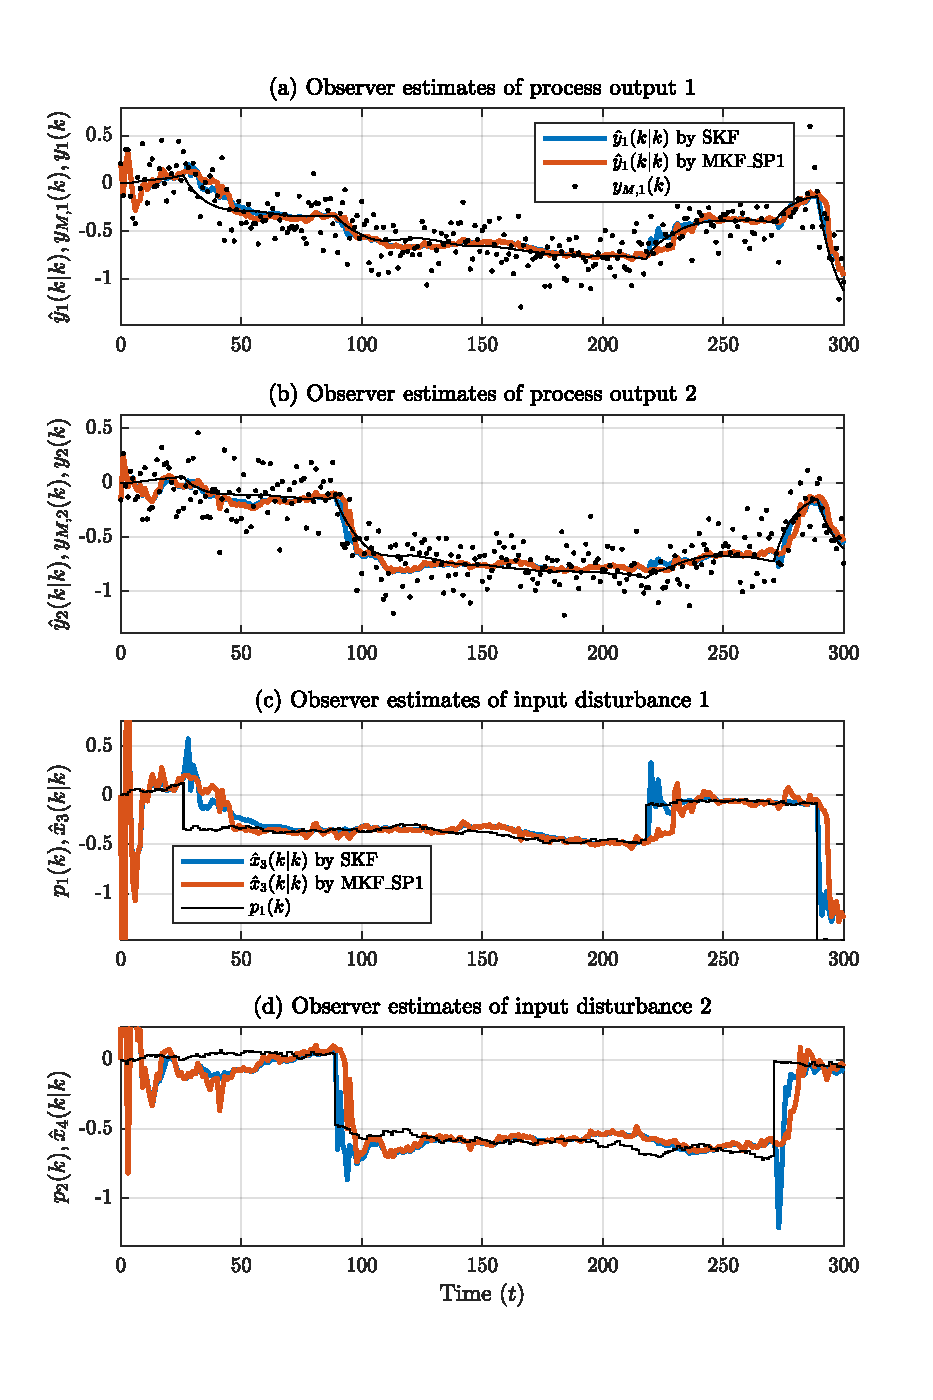
\includegraphics[width=13cm]{images/rod_obs_sim3_all_seed_y_est1_SP1.pdf}
	\caption{Estimates by sequence pruning observer –  $2\times2$ system}
	\label{fig:rod-obs-sim2-yest-1-SP}
\end{figure}

%\begin{figure}[htp]
%	\centering
%	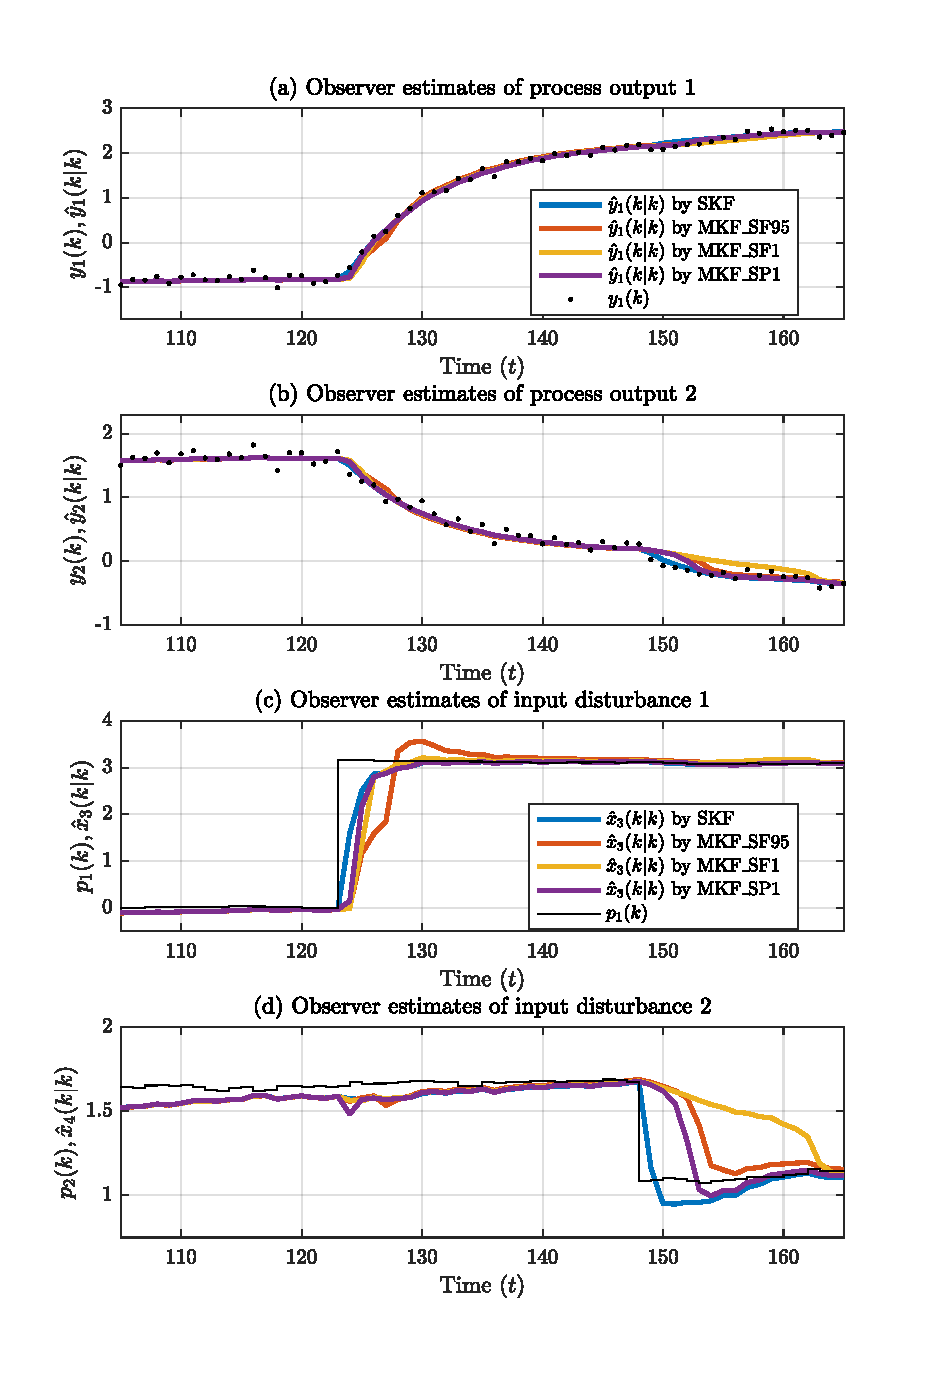
\includegraphics[width=13cm]{images/rod_obs_sim2_all_seed_y_est2_MKF.pdf}
%	\caption{Comparison of multiple-model observer estimates –  $2\times2$ system}
%	\label{fig:rod-obs-sim2-yest-2-MKF}
%\end{figure}
Figure \ref{fig:sim-sys-sim2-MKF-cumerr} shows the squared output estimation errors and the cumulative squared-errors of the five observers over the full simulation. This reveals that on average, the sequence fusion observers (MKF--SF95 and MKF--SF1) perform better than the sequence pruning observer. The cumulative errors of all the multiple model observers are significantly lower than those of KF3 by the end of the simulation, but not as close to those of the SKF as they were in the SISO system simulation. This may be attributed to the delays in detecting the shocks in this simulation.
\begin{figure}[htp]
	\centering
	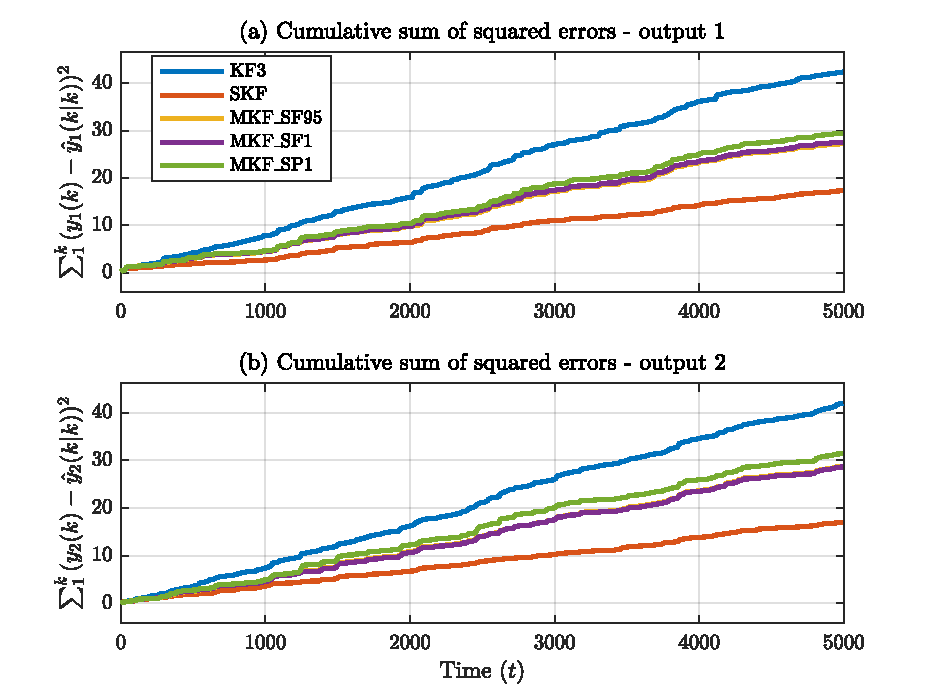
\includegraphics[width=13cm]{images/rod_obs_sim3_all_seed_cum_err_y2.pdf}
	\caption{Cumulative sum of squared errors of output estimates –  $2\times2$ system}
	\label{fig:sim-sys-sim2-MKF-cumerr}
\end{figure}

% Replaced with above single plot to save space
%\begin{figure}[htp]
%	\centering
%	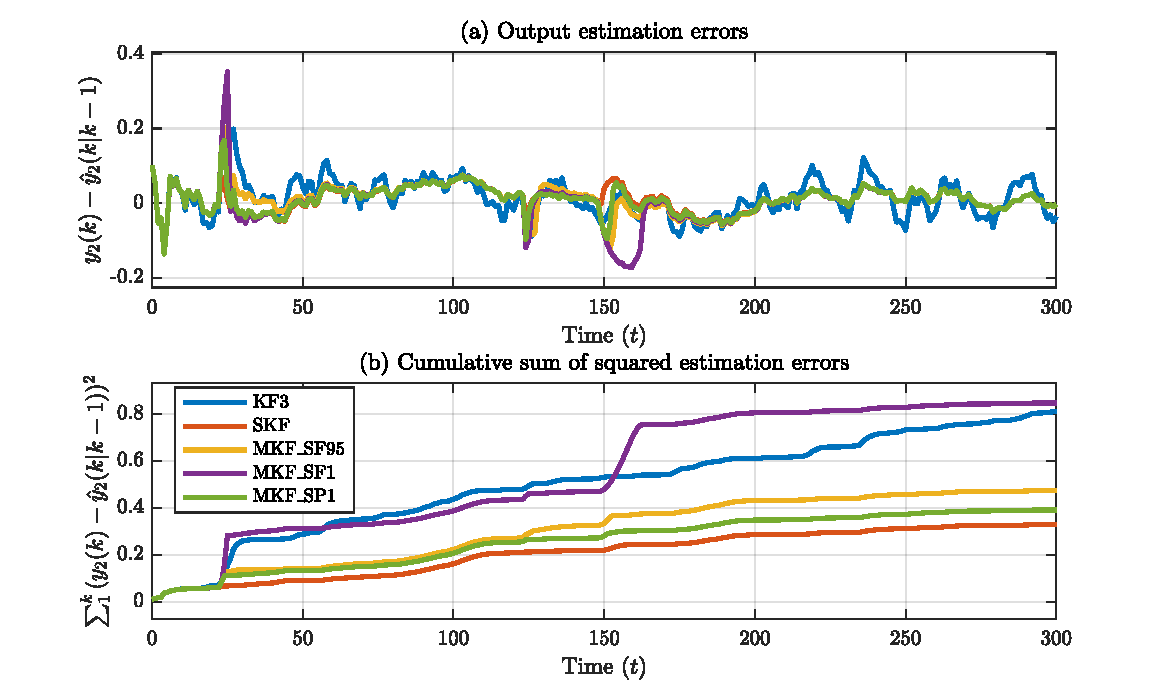
\includegraphics[width=13cm]{images/rod_obs_sim2_cum_err2.pdf}
%	\caption{Cumulative errors of multiple-model observer output estimates –  $2\t_y2mes2$ system}
%	\label{fig:sim-sys-sim2-MKF-cumerr2}
%\end{figure}
%\begin{figure}[htp]
%	\centering
%	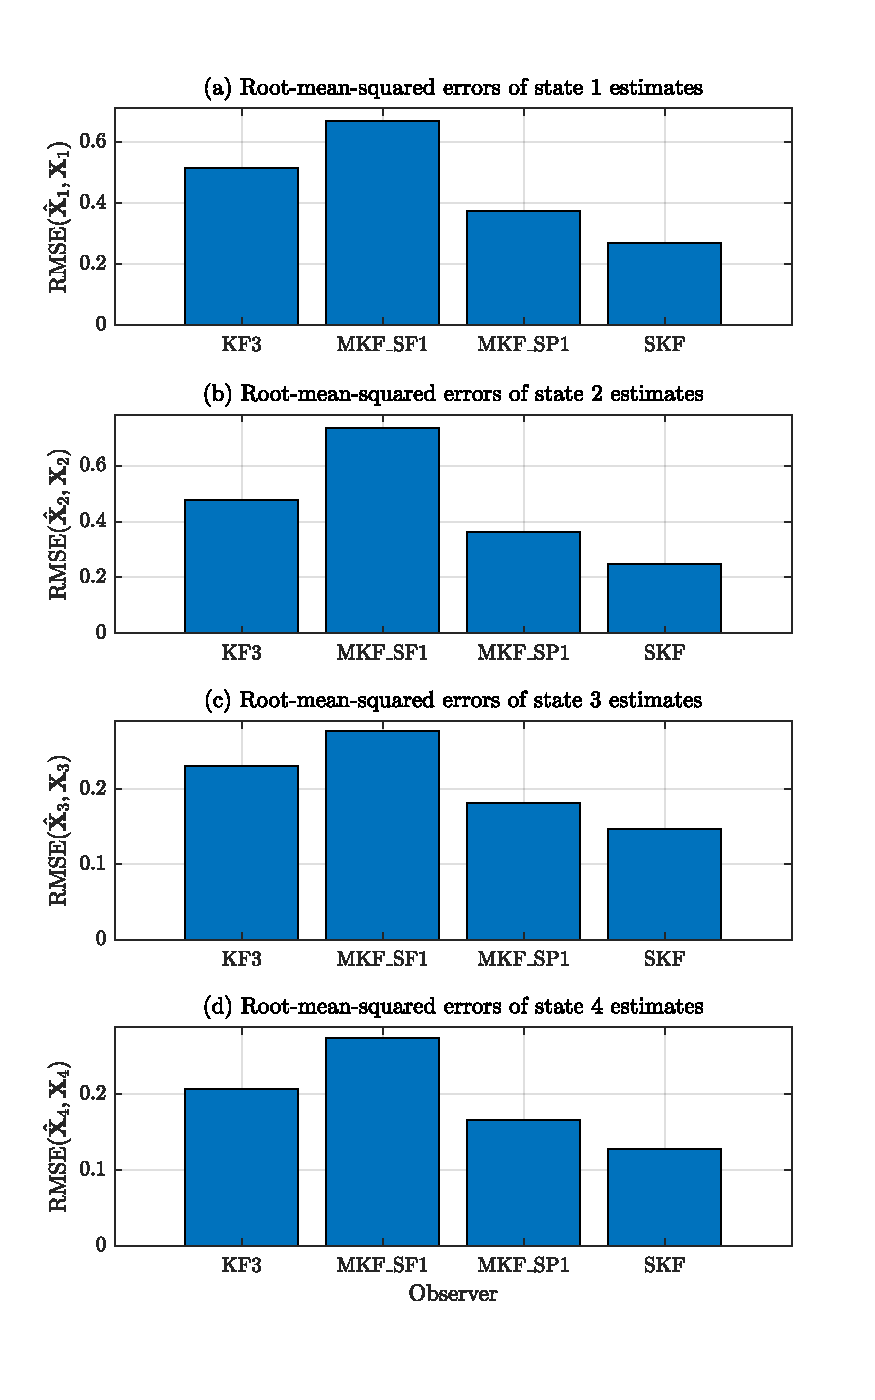
\includegraphics[width=11cm]{images/rod_obs_sim2_all_seed_x_err_bar.pdf}
%	\caption{Root-mean-squared errors of state estimates – $2\times2$ system}
%	\label{fig:rod-obs-sim2-xest-RMSE-bar}
%\end{figure}
As in the SISO case, 10 simulations were carried out with different random initializations to check the sensitivity of the results. Figure \ref{fig:rod-obs-sim2-yest-all-seed-RMSE-box} shows the variation in the RMSEs. This confirms that the performance of the three multiple-model observers is quite similar but MKF--SF95 and MKF--SF1 achieve a slightly lower error on average.
\begin{figure}[htp]
	\centering
	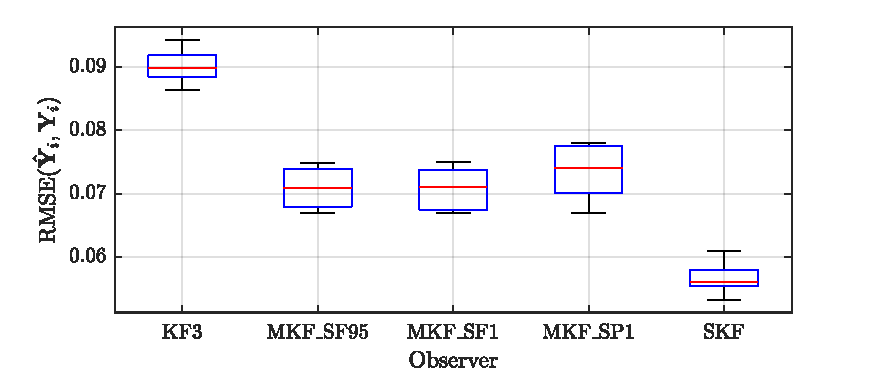
\includegraphics[width=12cm]{images/rod_obs_sim3_all_seed_y_err_box.pdf}
	\caption{Root-mean-squared errors of output estimates – $2\times2$ system}
	\label{fig:rod-obs-sim2-yest-all-seed-RMSE-box}
\end{figure}

\section{Grinding process simulations} \label{sec:sim-ore-SISO}

In this section, results of an experiment to test the observers with data from the grinding process simulator are presented. Unlike the simulations presented in section \ref{sec:sim-obs-lin}, the grinding simulator (described in Section \ref{sec:grinding-simulator}) is a non-linear model with a high number of state variables and complex dynamics based on a real grinding process.

This work is an extension of previously published work \citep{tubbs_observer_2022}. In the previous work, a multiple-model observer with sequence pruning was tested. Here, observers with sequence fusion and sequence pruning are evaluated and compared. Also, note that in the previous work, the prediction form of the Kalman filter (\ref{eq:xkp1_hat_p}) was used and the mean-squared errors (MSEs) of the estimates were compared, not the \gls{RMSE}s (\ref{eq:rmse-calc-yest}).

As in the previous work, the size of the ground product leaving the cyclone overflow was sampled at 3 minute intervals ($T_s=0.05$ hours) and a zero-mean Gaussian measurement noise with a standard deviation of 5 $\mu\text{m}$ was added directly to the simulator output. No other inputs were available to the observers. In total, data from 13 different runs of the simulation model were used. Table \ref{tb:grind1-sims} summarises the type of input signal used in each simulation, the duration, number of samples, and the simulation outputs that were used. The use of this data is described in the subsequent sections.
\begin{table}[ht]
	\begin{center}
		\caption{Grinding process simulations} \label{tb:grind1-sims}
		% See: https://texblog.org/2019/06/03/control-the-width-of-table-columns-tabular-in-latex/
		\begin{tabular}{
				>{\raggedleft\arraybackslash}p{0.32in}
				>{\centering\arraybackslash}p{0.8in}
				>{\centering\arraybackslash}p{0.6in}
				>{\centering\arraybackslash}p{0.6in}
				>{\centering\arraybackslash}p{0.8in}
				>{\raggedright\arraybackslash}p{1.8in}}
			\# & Input type & Duration (hours) & Samples ($N$) & Output data & Purpose \\
			\hline
			1 & \gls{PRBS} & 15 & 300 & $p(k),y_M(k)$ & Estimation of process model parameters \\
			2 & \gls{PRBS} & 15 & 300 & $p(k),y_M(k)$ & Validation of process models and model selection  \\
			3 & \gls{PRBS} & 15 & 300 & $p(k)$, $y(k)$, $y_M(k)$ & Figure \ref{fig:grind1_rod_obs_est_MKF_SF1}  \\
			6 & Random switching & 123 & 2460 & $y(k)$, $y_M(k)$ & Observer parameter selection \\
			6--15 & Random switching & 123 & 2460 & $y(k)$, $y_M(k)$ & Observer simulation and evaluation. \\
			\hline
		\end{tabular}
	\end{center}
\end{table}


\subsection{System identification} \label{sec:grind1-sysid}

The system model consists of a single-input, single-output (SISO) process model with a RODD step disturbance, $p(k)$, at the input, as shown in Figure \ref{fig:grind1_obs_model}.
\begin{figure}[ht]
	\centering
	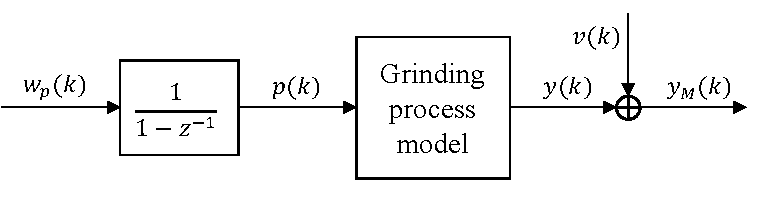
\includegraphics[width=9.5cm]{images/grind1-obs-model-diag.pdf}
	\caption{Observer model structure}
	\label{fig:grind1_obs_model}
\end{figure}
The output variable, $y(k)$, is the product P80. $v(k)$ is an additive measurement noise and $y_M(k)$ is the measurement.

To construct multiple-model observers for this system, the structure and parameters of the disturbance model and process model are needed. As mentioned in Section \ref{sec:sys-id}, standard system identification techniques are not suitable for estimating hybrid dynamical systems. To avoid this problem, it is assumed here that the time and magnitude of the disturbances (i.e. changes in the ore mix) have been determined for a period of time sufficient for identification of a process model. In practice, this might be possible by sampling the ore and carrying out a particle size analysis, or in the case where stocks of ores with known properties can be fed to the mill in a controlled manner for the duration of the data acquisition.

To mimic the system identification process as realistically as possible, three simulations were carried out (numbered 1--3 in Table \ref{tb:grind1-sims}) with a \textit{pseudo-random binary sequence} (\glsadd{PRBS}\gls{PRBS}) of step-changes in the ore mix factor and the process output measurements were recorded. Each simulation was started with the same initial state but run with a different disturbance input sequence, $p(0), p(1), ..., p(N)$. The simulations were of 15 hours duration ($N=300$) and the process was kept at steady-state for the first 3 hours of each simulation. The initial 3-hour period of the first simulation was used to estimate the normal operating point of the process. Each step in the \gls{PRBS} was one hour in duration. The lower plot in Figure \ref{fig:grind1-sim_ioplots} shows the values of $p(k)$ used in simulation 1. The simulated measurements, $y_M(k)$, are shown in the upper plot.
\begin{figure}[htp]
	\centering
	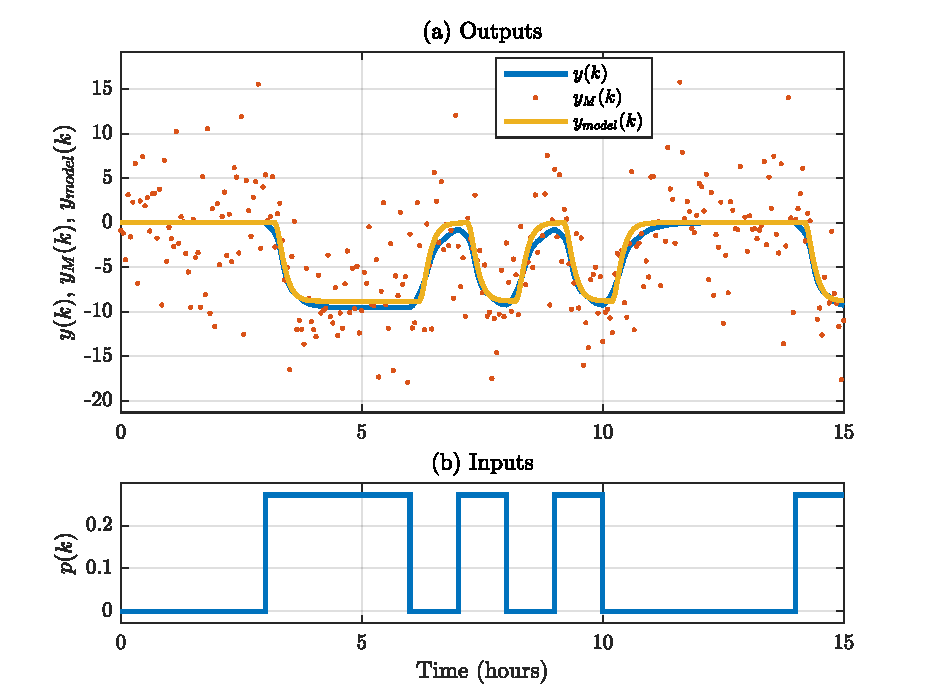
\includegraphics[width=13cm]{images/grind1_rod_obs_sim_1_ioplot_P2DcTd4.pdf}
	\caption{Simulation inputs and outputs}
	\label{fig:grind1-sim_ioplots}
\end{figure}

The Mathworks System Identification Toolbox™ was used to carry out the system identification. The data from simulation 1 was used to estimate the parameters of candidate process models. A model structure was selected after fitting a number of different models and calculating the prediction errors on the input-output data from simulation 2. After checking the significance of the estimated model parameters, a simple second-order model with a delay was selected. The transfer function of this model is
% Model name P2DcTd4
\begin{equation} \label{eq:grind1-id-model-ctf}
	G_p(s)= \frac{-32.4\exp(-0.2s)}{(1 + 0.106s)^2}.
\end{equation}
It has a delay of 0.2 hours (i.e. 4 sample periods, or 12 minutes) and a settling time (to within $\pm5\%$ of steady-state) of approximately 42 minutes. The upper plot in Figure \ref{fig:grind1-sim_ioplots} also shows the predictions of this model, $y_{model}(k)$, compared to the true output, $y(k)$. Note that there is a visible mismatch between the predictions of the identified linear model and the outputs of the grinding process simulator.

It was also assumed that the structure of the RODD model (\ref{eq:RODD}) was known, in this case a RODD step disturbance (\ref{eq:RODD-step}), and that values of the parameters $\sigma_{w_p}$, $b$, and $\epsilon$ were available. In practice, it should be possible to estimate $\epsilon$ from historic operating data by simply counting the number of ore changes in a sufficiently long period and dividing by the number of sample periods, although this method is somewhat inaccurate because small shocks are undetectable in noisy data. Estimating the magnitude of the shocks, $b$$\sigma_{w_p}$, could be more difficult. It may require prior knowledge of the true size distributions of the ores, perhaps from geological data or test work.

\subsection{Observer design} \label{sec:grind1-obs-design}

The discrete-time state-space representation of the augmented model (including RODD disturbance) used by the observers was
% P2DcTd4
\begin{multline} \label{eq:grind1-obs_ss_model}
	\mathbf{x}(k+1) = 
	\begin{bmatrix}
		1.248 & -0.7786 & 4 & 0 & 0 & 0 & 0 \\
		0.5   &  0      & 0 & 0 & 0 & 0 & 0 \\
		0     &  0      & 0 & 1 & 0 & 0 & 0 \\
		0     &  0      & 0 & 0 & 1 & 0 & 0 \\
		0     &  0      & 0 & 0 & 0 & 1 & 0 \\
		0     &  0      & 0 & 0 & 0 & 0 & 1 \\
		0     &  0      & 0 & 0 & 0 & 0 & 1 \\
	\end{bmatrix} \mathbf{x}(k)
	+ \begin{bmatrix}
		\mathbf{w}(k) \\
		w_p(k) \\
	\end{bmatrix}, \\
	y(k) = 
	\begin{bmatrix}
		-0.66214 & -0.96672 & 0 & 0 & 0 & 0 & 0 \\
	\end{bmatrix} \mathbf{x}(k) + \mathbf{v}(k) \\
\end{multline}
with a sampling period of 0.05 hours.

The noise covariance (\ref{eq:init_Q_R}) switched between two values,
\begin{equation} \label{eq:Q0}
	\begin{aligned}
		\mathbf{Q}_0=\begin{bmatrix}
			\sigma_{x_1}^2 & 0 & \cdots & 0 \\
			0 & \sigma_{x_2}^2 & \cdots & 0 \\
			\vdots & \vdots & \ddots & \vdots \\
			0 & 0 & \cdots & \sigma_{w_p}^2 \\
		\end{bmatrix}=\begin{bmatrix}
			0.01^2 & 0 & \cdots & 0 \\
			0 & 0.01^2 & \cdots & 0 \\
			\vdots & \vdots & \ddots & \vdots \\
			0 & 0 & \cdots & 0.002717^2
		\end{bmatrix}, \\
	\end{aligned}
\end{equation}
and 
\begin{equation} \label{eq:Q1}
	\begin{aligned}
		\mathbf{Q}_1=\begin{bmatrix}
			\sigma_{x_1}^2 & 0 & \cdots & 0 \\
			0 & \sigma_{x_2}^2 & \cdots & 0 \\
			\vdots & \vdots & \ddots & \vdots \\
			0 & 0 & \cdots & b^2\sigma_{w_p}^2 \\
		\end{bmatrix}=\begin{bmatrix}
			0.01^2 & 0 & \cdots & 0 \\
			0 & 0.01^2 & \cdots & 0 \\
			\vdots & \vdots & \ddots & \vdots \\
			0 & 0 & \cdots & 0.2717^2
		\end{bmatrix},
	\end{aligned}
\end{equation}
where $\sigma_{x_i}^2$ ($i=1,2,...,6$) are noise variance parameters of the process model states. Since model errors are not known in practice, an arbitrary value of  $0.01^2$ was chosen, although it did not have a significant impact on the results. In this work, the random shock variances, $\sigma_{w_p}^2$ and $b^2\sigma_{w_p}^2$, were set according to the simulated ore changes, as described below.

To evaluate the observers, longer simulations with randomly-occurring step changes in the ore mix factor were simulated. Each simulation consisted of an initial period of 3 hours at steady-state followed by 120 hours (equivalent to 5 days) of randomly-occurring step changes. Note that this is not a RODD according to the definition because the magnitude of the shocks is not random. RODDs are unbounded and therefore not realistic representations of actual process disturbances, which are unlikely to be Gaussian random variables. Instead, a simple switching ore mix factor, \glsadd{porek}\gls{porek}, was used. \gls{porek} is a discrete random variable with two possible values, that switches according to the shock probability \gls{epsilon}. It can be represented by a \gls{HMM} with one binary state, \gls{rk}, such that
\begin{equation} \label{eq:pk-grind}
	p_\text{ore}(k) = \begin{cases*}
		0.2283 & if $r(k)=1$, \\
		0.5 & if $r(k)=2$,
	\end{cases*} \\
\end{equation}
and with the transition probability matrix
\begin{equation} \label{eq:Pi-rk-grind}
	\glsadd{Piwp}\Pi_{p_\text{ore}} = \begin{bmatrix}
		1-\epsilon & \epsilon \\
		\epsilon & 1-\epsilon
	\end{bmatrix}.
\end{equation}

The parameters of the RODD model used in the observer design were chosen in the following way. Although the probability density of $p_\text{ore}(k)$ is obviously not Gaussian, it has a conditional standard deviation of either 0.2717 (the difference between 0.5 and 0.2283) or 0. Based on this, $b\sigma_{w_p}$ was set to 0.2717 and \gls{b} was arbitrarily set to 100, meaning that \gls{sigmawp} was 0.002717. \gls{epsilon} was set to 0.01, which was the true value used in (\ref{eq:Pi-rk-grind}) to simulate $p_\text{ore}(k)$. $\epsilon=0.01$ means that, on average, an ore change occurred every 100 sample periods, or every 5 hours.

Three multiple-model observers were designed using a similar method to that described in Section \ref{sec:sim-obs-lin-1-MKF-tuning}. It was found that large data sets from long simulations were necessary to obtain good combinations of parameter values for these observers. When this was attempted with shorter data sets like simulations 1--3, the results were variable, and the performance of the observers was often poor. This can be explained by the fact that shocks are infrequent, and also that the sequence fusion algorithms in particular, are somewhat sensitive to the exact timing of shocks. The simulations must be long enough to provide a sufficient number and diversity of shock sequences to avoid `overfitting' the parameters to the data.

For this reason, data from one of the longer simulations was used (number 6) to obtain the parameter values of the observers evaluated below. This simulation was 5 days in duration (2460 samples), simulated with $p_\text{ore}(k)$ as the input, and included 32 step changes. This was sufficient to obtain good parameter values. Note that the true values of the disturbance are not needed for observer parameter selection.

However, in practice it would not be possible to use the true process outputs because they are unknown. In that case, the parameter tuning would have to be done using the \gls{RMSE} of the measured outputs, $\text{RMSE}(\hat{\mathbf{Y}}(N), \mathbf{Y}_M(N))$. The true outputs from the simulation model were used in this experiment to ensure the best possible parameter values were obtained and thus allow a more reliable comparison of the possible performance of each observer type.

The performance of the multiple-model observers was again compared to a standard Kalman filter labelled `KF3', with a manually-tuned covariance matrix,
\begin{equation} \label{eq:Q_opt}
	\mathbf{Q}_{opt}=\begin{bmatrix}
		0.01^2 & \cdots & 0 & 0 \\
		\vdots & \ddots & \vdots & \vdots \\
		0 & \cdots & 0.01^2 & 0 \\
		0 & \cdots & 0 & 0.0234^2
	\end{bmatrix}.
\end{equation}

$\mathbf{Q}_{opt}$ was found to produce the lowest average error of the output estimates, $\text{RMSE}(\hat{\mathbf{Y}}(N),\mathbf{Y}(N))$, when simulated on the data from simulation number 6.

All three observers used the same initial covariance of the state estimates:
\begin{equation} \label{eq:P0}
	\mathbf{P}_0=\begin{bmatrix}
		0.1 & \cdots & 0 & 0 \\
		\vdots & \ddots & \vdots & \vdots \\
		0 & \cdots & 0.1 & 0 \\
		0 & \cdots & 0 & 0.01
	\end{bmatrix}.
\end{equation}

%TODO: Summarize the comparison of the observers over all simulations at the end.
Table \ref{tb:grind1-obs-params-sim1} is a summary of the parameters of the four observers chosen for evaluation.
\begin{table}[ht]
	\begin{center}
		\caption{Observer parameters for grinding process simulation.} \label{tb:grind1-obs-params-sim1}
		% See: https://texblog.org/2019/06/03/control-the-width-of-table-columns-tabular-in-latex/
		\begin{tabular}{p{0.16\textwidth}>{\centering\arraybackslash}p{0.12\textwidth}>{\centering\arraybackslash}p{0.16\textwidth}>{\centering\arraybackslash}p{0.16\textwidth}>{\centering\arraybackslash}p{0.16\textwidth}}
			& KF3 & MKF--SF95 & MKF--SF1 & MKF--SP \\
			\hline
			Type & Kalman filter & Multi-model Kalman filter & Multi-model Kalman filter & Multi-model Kalman filter \\
			Algorithm & - & Sequence fusion 95 & Sequence fusion 98 & Sequence pruning \\
			\hline
			Parameters &  &  &  &  \\
			\gls{Qset} & $\mathbf{Q}_{opt}$ & $\{\mathbf{Q}_0,\mathbf{Q}_1\}$ & $\{\mathbf{Q}_0,\mathbf{Q}_1\}$ & $\{\mathbf{Q}_0,\mathbf{Q}_1\}$ \\
			\gls{R} & $5^2$ & $5^2$ & $5^2$ & $5^2$ \\
			$\mathbf{P}(0)$ & $\mathbf{P}_0$ & $\mathbf{P}_0$ & $\mathbf{P}_0$ & $\mathbf{P}_0$ \\
			\gls{nh} & 1 & 34 & 26 & 25 \\
			\gls{nf} & - & 60 & 60 & - \\
			\gls{m} & - & 2 & 2 & - \\
			\gls{d} & - & 10 & 12 & - \\
			\gls{nmin} & - & - & - & 23 \\
			\gls{epsilon} & - & 0.01 & 0.01 & 0.01 \\
			\gls{sigmawp} & - & 0.002717 & 0.002717 & 0.002717 \\
			\gls{b} & - & 100 & 100 & 100 \\
			\hline
		\end{tabular}
	\end{center}
\end{table}

\subsection{Simulation results} \label{sec:grind1-sim-results}

Figure \ref{fig:grind1_rod_obs_est_MKF_SF1} shows the estimates of the sequence fusion observer, MKF--SF1, compared to the Kalman filter and the true system outputs. Only the estimates of MKF--SF1 are shown here because this had the lowest estimation errors. The estimates of the other two MKF observers were very similar. Note that the data used in this simulation was not used for either system identification or observer parameter selection. From the upper plot it is clear that the measurement noise level is higher than in the previous simulations, relative to the magnitude of the changes in the system outputs. The estimates of both observers lag the true outputs after step changes in the disturbance. It is unclear from this plot whether the multiple-model observer has a significant performance advantage over the Kalman filter. The \gls{MKF} observer estimates seem to fluctuate less during steady-state periods, for example, immediately before the first step change. However, the differences are not as obvious as they were in the linear system simulations.
\begin{figure}[htp]
	\centering
	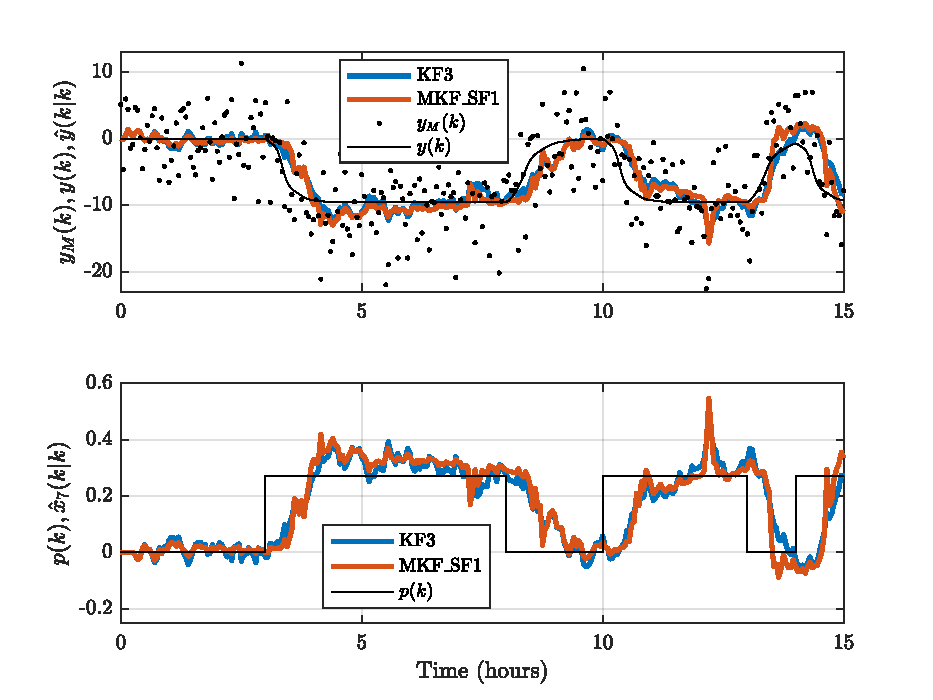
\includegraphics[width=13cm]{images/grind1_rod_obs_sim_3_est_MKF_SF1.pdf}
	\caption{Observer estimates -- MKF--SF1}
	\label{fig:grind1_rod_obs_est_MKF_SF1}
\end{figure}
Occasionally, rapid changes occur in the estimates of both observers even when there is no disturbance. This may be attributed to extreme values in the measurement noise which occurred at certain times.

As in the previous experiments, longer simulations are needed to evaluate the observers. This was achieved using data from 10 simulations, similar to and including simulation number 6 but generated from unique pseudo-random initializations. These simulations were numbered 6 to 15 as shown in Table \ref{tb:grind1-sims}. In addition to the metrics defined in \ref{sec:evaluation}, two additional \gls{RMSE} metrics were devised for this experiment. Firstly, an \gls{RMSE} during \textit{transient periods} when the system was responding to a disturbance. Transient periods were defined as sample times occurring after a step change and before the end of the settling time of the process. The settling time of the process, \glsadd{tset95}\gls{tset95}, was defined as the longest time taken for the process to reach within $\pm5\%$ of a steady-state after a step change in the input. The longest settling time was found to be approximately 1.2 hours when the process was switching from ore mix \#2 to mix \#1. The second additional metric is the \gls{RMSE} during \textit{steady-state periods}, which were defined as sample times occurring more than 1.2 hours after one disturbance and before the next. 

\begin{table}[ht]
	\begin{center}
		\caption{Observer performance evaluation metrics.} \label{tb:grind1-RMSE-results}
		% See: https://texblog.org/2019/06/03/control-the-width-of-table-columns-tabular-in-latex/
		\begin{tabular}{p{0.29\textwidth}>{\centering\arraybackslash}p{0.08\textwidth}>{\centering\arraybackslash}p{0.14\textwidth}>{\centering\arraybackslash}p{0.12\textwidth}>{\centering\arraybackslash}p{0.12\textwidth}>{\centering\arraybackslash}p{0.08\textwidth}}
			Metric & KF3 & MKF--SF95 & MKF--SF1 & MKF-SP & SKF \\
			\hline
			%			% 09-Dec-2022 11:35:30 results with system P2DcTd4, sigma_M = 5 - but horizon limit was 50
			%			RMSE($\hat{\mathbf{Y}},\mathbf{Y}$) overall & 1.81 & 1.69 & 1.66 & 1.70 & 1.24 \\
			%			RMSE($\hat{\mathbf{Y}},\mathbf{Y}$) transient & 2.51 & 2.81 & 2.76 & 2.94 & 2.00 \\
			%			RMSE($\hat{\mathbf{Y}},\mathbf{Y}$) steady-state & 1.54 & 1.14 & 1.11 & 1.06 & 0.89 \\
			%			Var($\hat{\mathbf{Y}}$) steady-state & 1.82 & 0.73 & 0.68 & 0.53 & 0.23 \\
			%			RMSD($\hat{\mathbf{Y}},\mathbf{Y}$) steady-state &0.69 & 0.46 & 0.45 & 0.43 & 0.17 \\
			%			% See script rod_obs_calc_metrics.m
			%			% 10-Dec-2022 09:14:50 results with system P2DcTd4, sigma_M = 5 after inc. horizon limit to 100
			%			RMSE($\hat{\mathbf{Y}},\mathbf{Y}$) overall & 1.81 & 1.70 & 1.66 & 1.67 & 1.24 \\
			%			RMSE($\hat{\mathbf{Y}},\mathbf{Y}$) transient & 2.51 & 2.88 & 2.77 & 2.86 & 2.00 \\
			%			RMSE($\hat{\mathbf{Y}},\mathbf{Y}$) steady-state & 1.54 & 1.10 & 1.11 & 1.07 & 0.89 \\
			%			Var($\hat{\mathbf{Y}}$) steady-state & 1.82 & 0.63 & 0.67 & 0.55 & 0.23 \\
			%			RMSD($\hat{\mathbf{Y}},\mathbf{Y}$) steady-state &0.69 & 0.43 & 0.45 & 0.43 & 0.17 \\
			% See script rod_obs_calc_metrics.m
			% 10-Dec-2022 15:43:28 results with system P2DcTd4, sigma_M = 5, after re-tuning KF3
			RMSE($\hat{\mathbf{Y}},\mathbf{Y}$) overall & 1.81 & 1.70 & 1.66 & 1.67 & 1.24 \\
			RMSE($\hat{\mathbf{Y}},\mathbf{Y}$) transient & 2.63 & 2.88 & 2.77 & 2.86 & 2.00 \\
			RMSE($\hat{\mathbf{Y}},\mathbf{Y}$) steady-state & 1.46 & 1.10 & 1.11 & 1.07 & 0.89 \\
			Var($\hat{\mathbf{Y}}$) steady-state & 1.60 & 0.63 & 0.67 & 0.55 & 0.23 \\
			RMSD($\hat{\mathbf{Y}},\mathbf{Y}$) steady-state &0.62 & 0.43 & 0.45 & 0.43 & 0.17 \\
			\hline
		\end{tabular}
	\end{center}
\end{table}
Table \ref{tb:grind1-RMSE-results} shows the values of the five metrics for the five observers when evaluated on the data from the 10 longer simulations. In terms of the overall \gls{RMSE}s, the multiple-model observers offer only a marginal improvement compared to the Kalman filter (which was tuned to minimize overall \gls{RMSE}). MKF--SF1 has the lowest overall \gls{RMSE}, which is 8.3\% lower than that of KF3. However, it is 39\% higher than that of the scheduled Kalman filter (SKF). The greater difference between the performance of the SKF and the other observers in this simulation may be attributed at least in part to the discrete-time delays in the process model (\ref{eq:grind1-obs_ss_model}) (it is impossible for any observer to respond to an input disturbance before its effect has reached the measured outputs, leading to inevitable estimation errors).

The other metrics in Table \ref{tb:grind1-RMSE-results} allow the specific strengths and weaknesses of each observer to be compared. In terms of transient errors, the multiple-model observers are inferior to KF3, with 5.3 to 9.5\% higher \gls{RMSE}s. However, in steady-state periods, they perform significantly better, with 24.0 to 26.7\% lower RMSEs. The \gls{RMSD}s of the multiple-model observers are 27.4 to 30.7\% lower, suggesting that insensitivity to measurement noise may be their main advantage. A reduced sensitivity to noise, combined with low transient errors would be beneficial in a feedback control application where the closed-loop response time is limited by the speed of the observer and where sensitivity to noise causes problems for actuators.

To provide further insight into the transient behaviour of one of the observers, 100 responses of the sequence fusion observer MKF-SF1 to step disturbances, were selected from simulations 6 to 15. The selected step changes were those when the system was in steady-state with ore mix \#1 when a step change occurred to mix \#2 and the process subsequently reached steady-state. The response sequences were aligned by subtracting the step time, \glsadd{tstep}\gls{tstep}, from the times of each response. Then the mean, minimum, and maximum values of the observer output estimates were calculated at each sample time since the step change. The results are shown in Figure \ref{fig:sim_resp_plot_MKF_SF1} as a thick orange line representing the average of the responses, and a pale orange area indicating the minima and maxima. Similar data for the Kalman filter, KF3, and the true system output are superimposed in the plot. This allows both the average (i.e. expected) observer response and the range of the variation that occurred, to be visualised and compared.
%\begin{figure}[htp]
%	\centering
%	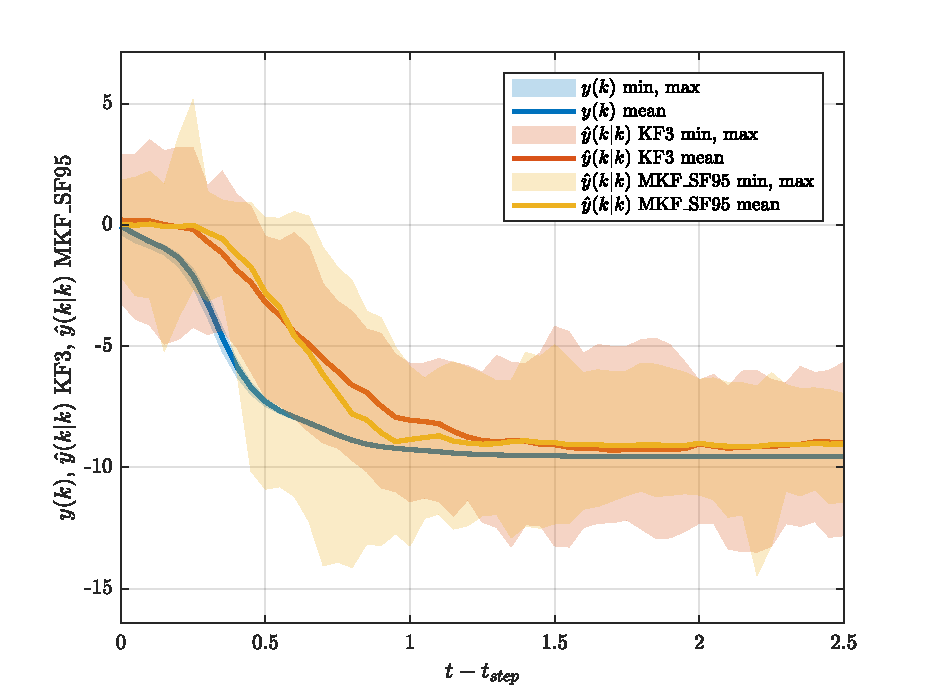
\includegraphics[width=12cm]{images/grind1_rod_obs_sim_resp_plot1_MKF_SF95.pdf}
%	\caption{Average observer responses to step disturbances -- MKF--SF95}
%	\label{fig:sim_resp_plot_MKF_SF95}
%\end{figure}
\begin{figure}[htp]
	\centering
	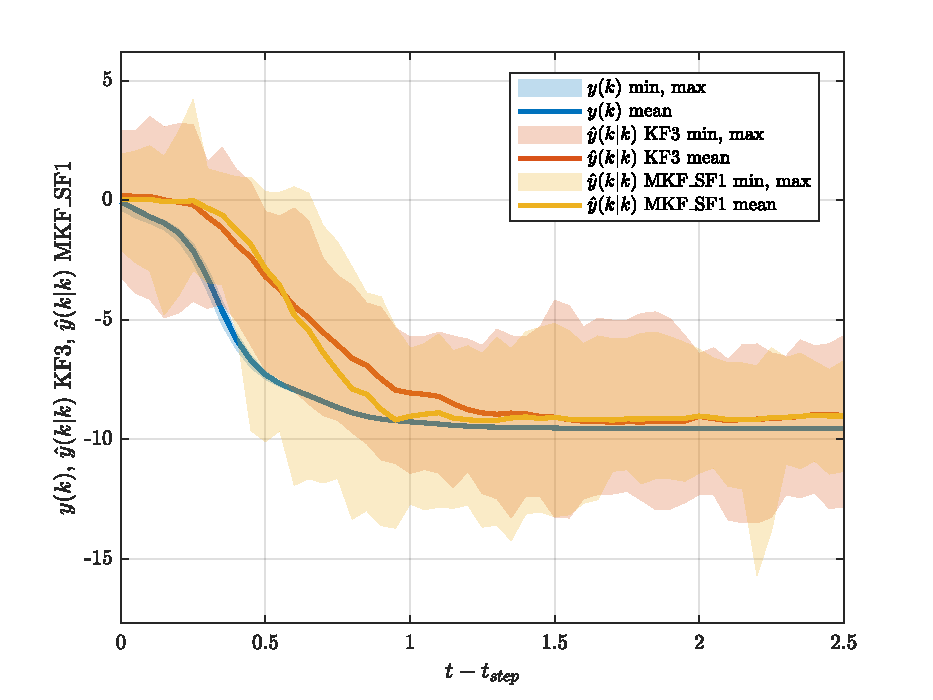
\includegraphics[width=13cm]{images/grind1_rod_obs_sim_resp_plot1_MKF_SF1.pdf}
	\caption{Average observer responses to step disturbances -- MKF--SF1}
	\label{fig:sim_resp_plot_MKF_SF1}
\end{figure}
%\begin{figure}[htp]
%	\centering
%	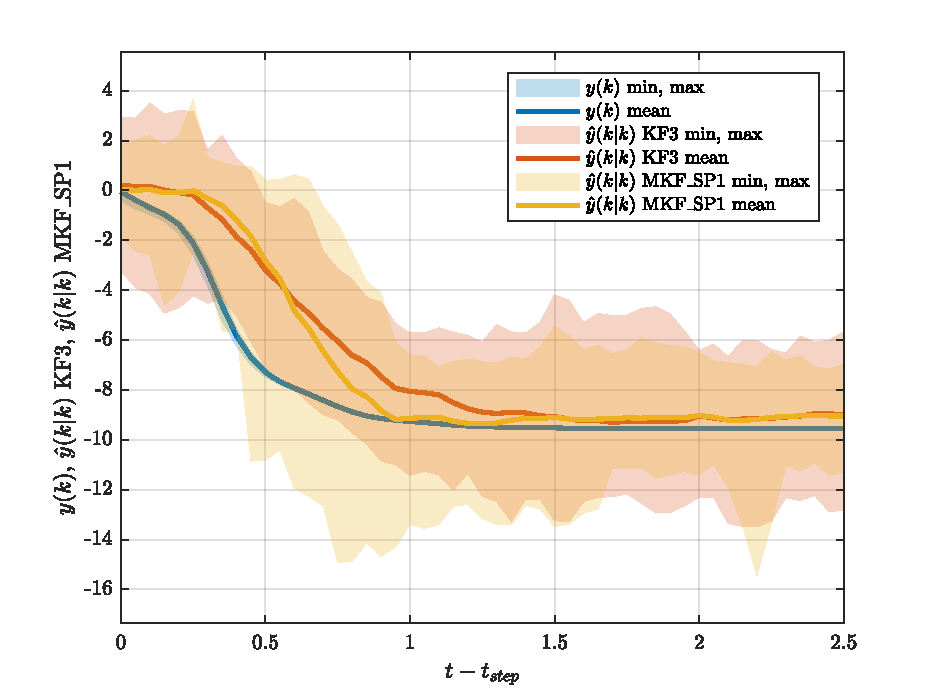
\includegraphics[width=12cm]{images/grind1_rod_obs_sim_resp_plot1_MKF_SP1.pdf}
%	\caption{Average observer responses to step disturbances -- MKF--SP}
%	\label{fig:sim_resp_plot_MKF_SP}
%\end{figure}
Figure \ref{fig:sim_resp_plot2_MKF_SF1} is a similar plot produced in the same way for the reverse steps when the process switched from ore mix \#2 to \#1.
\begin{figure}[htp]
	\centering
	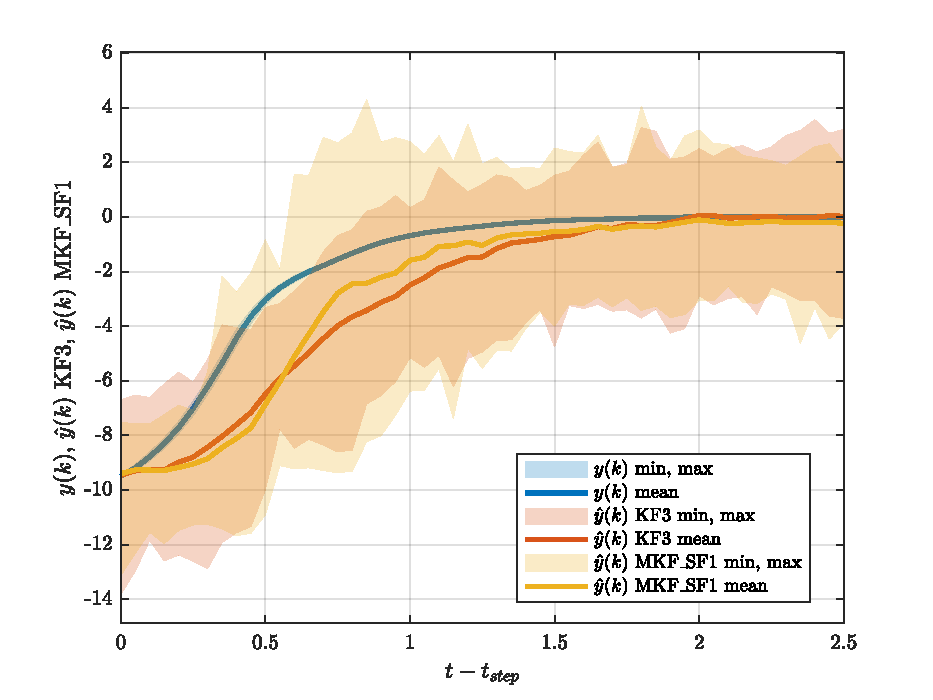
\includegraphics[width=13cm]{images/grind1_rod_obs_sim_resp_plot2_MKF_SF1.pdf}
	\caption{Average observer responses to step disturbances -- MKF--SF1}
	\label{fig:sim_resp_plot2_MKF_SF1}
\end{figure}

Figures \ref{fig:sim_resp_plot_MKF_SF1} and \ref{fig:sim_resp_plot2_MKF_SF1} reveal a few interesting characteristics of the multiple-model observer. Firstly, the average response has a characteristic `S'-shape when compared to that of KF3. It is initially slightly slower to respond, then overtakes the response of KF3 and reaches the vicinity of the true system output significantly earlier. This can be explained by the bi-modal behaviour of the multiple-model observer, which is insensitive to noise most of the time but has a high correction gain once a shock is detected. However, the average response is not representative of individual responses. It can seen from the minimum and maximum values that during the transition period, the multiple-model observer exhibits high variation and often larger estimation errors than the Kalman filter. Around 1.5 hours after the shocks, the variation in the estimates of MKF--SF1 reduces to less than that of KF3. 

\subsection{Sensitivity analysis} \label{sec:grind1-sensitivity-analysis}
Finally, an analysis was carried out to investigate the sensitivity of the observer performance to selected parameters. Firstly, the sensitivity of the overall \gls{RMSE}s to the process model parameters was analysed. The continuous-time linear process model identified from simulation data (\ref{eq:grind1-id-model-ctf}) was generalised by introducing two adjustable parameters, a static gain, \glsadd{Kp}\gls{Kp}, and a time constant, \glsadd{Tp1}\gls{Tp1},
\begin{equation} \label{eq:grind1-id-model-ctf}
	G_p(s)= \frac{K_p \exp(-0.2s)}{(1 + T_{p,1})^2}.
\end{equation}

The process delay of 0.2 hours remained fixed. Each parameter was than adjusted according to a set of 7 ratios from 0.5 to 2 (including 1) and the adjusted models were used in the observers and simulated using data set number 6. Since all possible combinations of both parameter values were considered, there were $7\times7=49$ simulations. After each simulation, the ratios of the overall \gls{RMSE} of each observer, to that with the original parameter values were calculated. The results are shown in Figure \ref{fig:grind1-obs-sim-sens-model-y-est} as percentage differences, with a colour-mapping to indicate the magnitude of the changes.
\begin{figure}[htp]
	\centering
	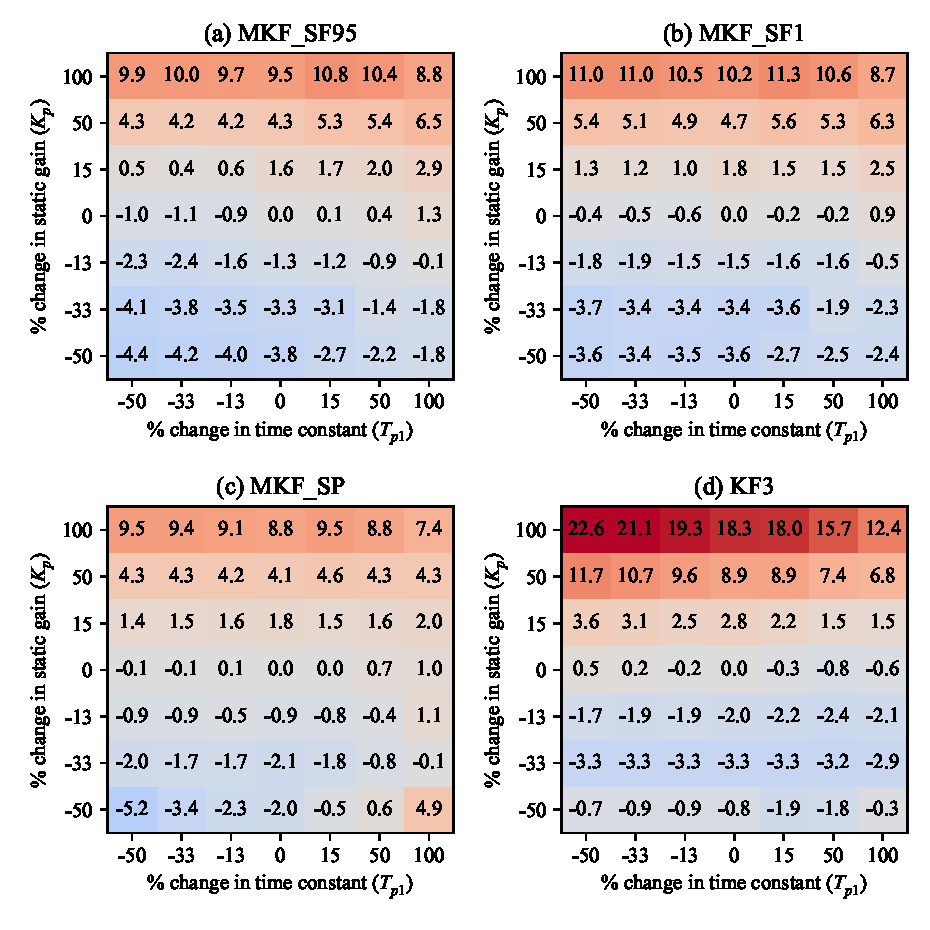
\includegraphics[width=15cm]{images/rod_obs_sim_sens_sys_4obs_RMSE_y_est.pdf}
	\caption{Percentage changes in RMSEs due to changes in process model parameters}
	\label{fig:grind1-obs-sim-sens-model-y-est}
\end{figure}

From these results it can be seen that the average magnitude of the estimation errors of the multiple-model observers varied by -5.2 to +11.3\% over the range of parameter values simulated. The highest errors occurred when the process gain, \gls{Kp} was doubled. The effect of changes in the time constant, \gls{Tp1}, was less significant.

By comparing these variations to those of KF3, it can be seen that the multiple-model observers are less sensitive to the model parameters. The few cases where the changes in the performance of the multiple-model observers are larger, are all cases where the estimation errors were lower than the KF3, therefore better performance. Based on this, there does not appear to be a significant downside to the multiple-model observers when it comes to the accuracy of the process model. In fact, it shows that better overall estimation performance may have been possible with different parameter values.

In the second part of this analysis, the sensitivity of the observer performance to the \gls{RODD} model parameters, \gls{sigmawp} and \gls{epsilon}, was investigated. The two parameters were adjusted in the same way as in the previous analysis and the changes in the overall \gls{RMSE}s calculated. The results are shown in Figure \ref{fig:grind1-obs-sim-sens-rod-y-est}. Note that the Kalman filter does not include a RODD model and was therefore excluded. Instead, the sensitivity of the scheduled Kalman filter, SKF, was included for comparison.
\begin{figure}[htp]
	\centering
	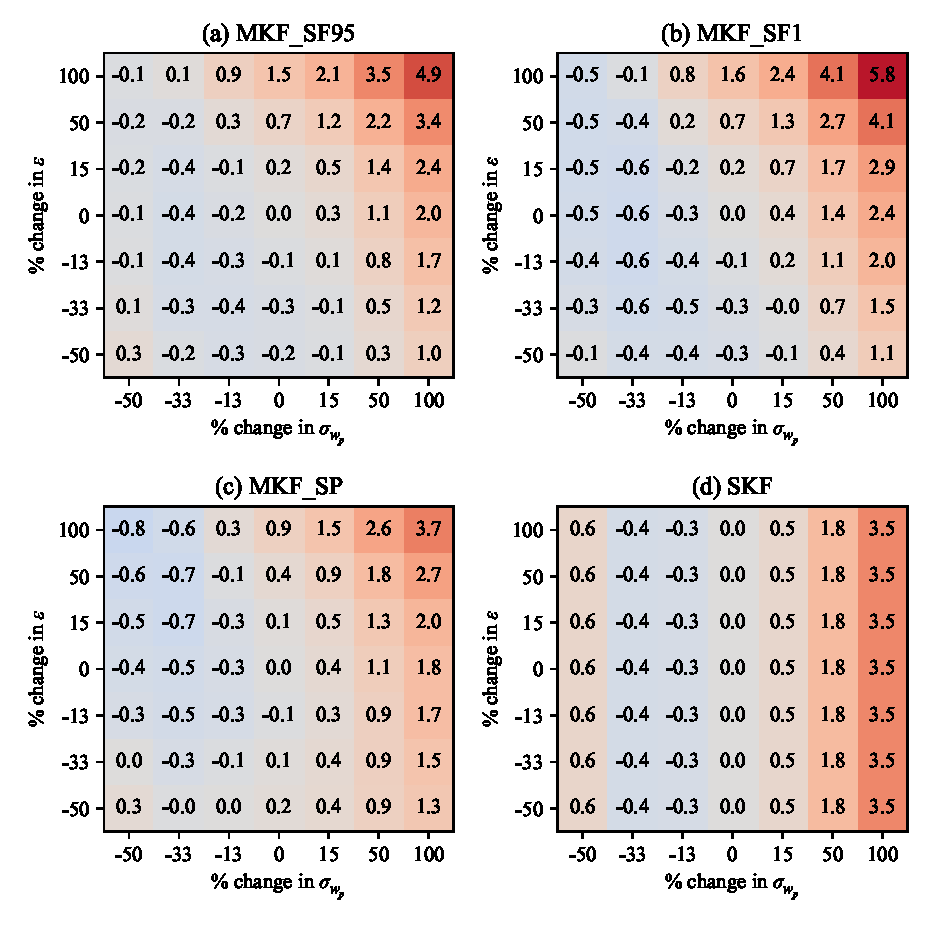
\includegraphics[width=15cm]{images/rod_obs_sim_sens_rod_4obs_RMSE_y_est.pdf}
	\caption{Percentage changes in RMSEs due to changes in \gls{RODD} parameters}
	\label{fig:grind1-obs-sim-sens-rod-y-est}
\end{figure}
Note that the SKF has the true shock sequence and therefore does not depend on \gls{epsilon}. From these results it can be seen that the average magnitude of the estimation errors of the multiple-model observers varied by -0.8 to +5.8\% over the range of parameter values simulated. The highest errors occurred when both \gls{sigmawp} and \gls{epsilon} were double their original values.


%\section{Grinding circuit control simulation} \label{sec:sim-ore-mimo-ctrl} 
%
%Outline notes:
%\begin{itemize}
%	\item Grinding simulation model in closed loop with \gls{MPC} controller.
%	\item Diagram of feedback system – Figure \ref{fig:sim-mpc-diag}
%	\item Table of results - Performance metrics — e.g. tracking error.
%	\item Robustness?  E.g. stability margins.
%\end{itemize}
%
%\begin{figure}[htp]
%	\centering
%	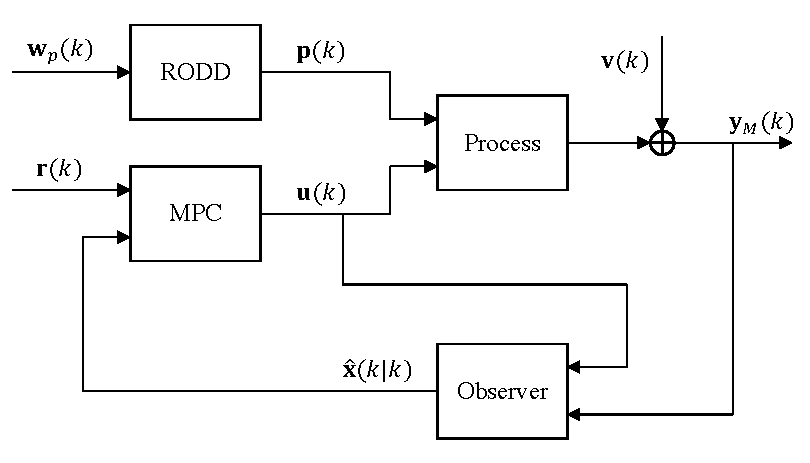
\includegraphics[width=11cm]{images/sim-mpc-diag.pdf}
%	\caption{Functional diagram of the simulated feedback control system}
%	\label{fig:sim-mpc-diag}
%\end{figure}
%
%\begin{figure}[htp]
%	\centering
%	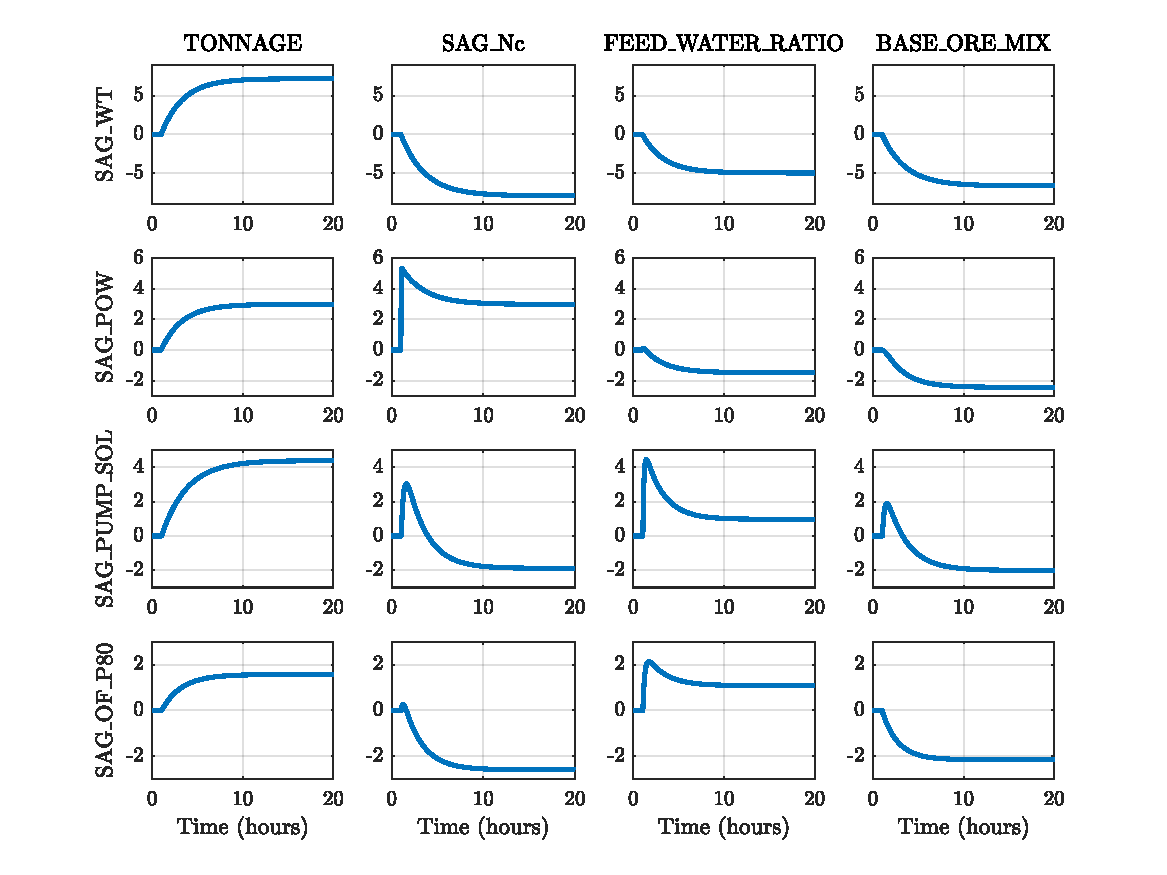
\includegraphics[width=15.5cm]{images/mpc4x4_stepresp_matrix.pdf}
%	\caption{Step responses of identified input-output model}
%	\label{fig:mpc4x4-stepresp-matrix}
%\end{figure}

